% The original is from UDESC
% Lambd0x (Nicholas P. Lane) changed it
% Now I am using it

\NeedsTeXFormat{LaTeX2e}

\documentclass[a4paper,12pt]{monografia}
\usepackage{amsmath, amsthm, amsfonts, amssymb}
\usepackage[english, brazilian]{babel}
\usepackage[titletoc]{appendix}
\usepackage[utf8]{inputenc}
\usepackage[T1]{fontenc}
\usepackage[mathcal]{eucal}
\usepackage[alf]{abntcite}
\usepackage[font=small,labelfont=bf,tableposition=top]{caption}
%\usepackage{subfig}
\usepackage{subcaption}
\usepackage{isoaccent}
\usepackage{textcase}
\usepackage{multirow}
\usepackage{latexsym}
\usepackage{graphicx}
\usepackage{listings}
\usepackage{acronym}
\usepackage{csquotes}
\usepackage[table,xcdraw]{xcolor}

\usepackage{enumitem}
\usepackage{url}

\usepackage{bm}

\setlist[description]{leftmargin=\parindent,labelindent=\parindent}

\lstset{basicstyle=\tiny, language=C++}

\makeindex

\setcounter{secnumdepth}{5}


\begin{document}

\titulo{Otimiza��es para Motores de Jogos Atrav�s de Modelagem Orientada a Dados}
\autor{Vin�cius Bruch Zuchi}
\nome{Vinicius Bruch}
\ultimonome{Zuchi}

\bacharelado \curso{Ci\^encia da Computa\c{c}\~ao} \mes{Junho} \ano{2016}
\data{\today}
\cidade{Joinville}

\instituicao{Universidade do Estado de Santa Catarina}
\sigla{UDESC} \unidadeacademica{Centro de Ci\^encias Tecnol\'ogicas}

\orientador{Andr� Tavares da Silva}
\examinadorum{Gilm�rio Barbosa dos Santos}
\examinadordois{Roberto Silvio Ubertino Rosso}
\examinadortres{Diego Buchinger}

\ttorientador{Doutor}
\ttexaminadorum{Doutor}
\ttexaminadordois{Doutor}
\ttexaminadortres{Mestre}

\maketitle

\agradecimento{Agradecimentos}

Agrade�o o professor Andr� Tavares da Silva, pela orienta��o, ajuda no desenvolvimento,
sugest�es e ideias para este trabalho.

Agrade�o tamb�m os meus pais, Edson e Neusa, pelo apoio e suporte que me deram ao longo 
dos meus �rduos anos de faculdade.

Por fim, agrade�o os meus amigos Karll e Renan, por terem me ajudado e encorajado na 
escolha do tema deste trabalho.

\newpage

\begin{epigrafe}

    ``Perseverance is the hard work you do after you get tired of doing the hard work 
    you already did'' - Newt Gingrich

\end{epigrafe}

\resumo{Resumo}
Devido � diferen�a de desempenho entre os microprocessadores e a velocidade de acesso 
� mem�ria principal, muitas aplica��es de computador modernas t�m sofrido com um problema 
conhecido como gargalo do processador-mem�ria, no qual o processador fica ocioso aguardando 
dados serem buscados na mem�ria. Aplica��es gr�ficas, principalmente jogos eletr�nicos, s�o 
not�rias por sofrerem deste problema pela demasiada quantidade de elementos diferentes que as 
constituem. Este trabalho prop�e a implementa��o de um motor de jogos (uma \textit{engine}) 
utilizando um conceito de estrutura��o de c�digo, a modelagem orientada a dados, com a 
finalidade de amenizar este problema de gargalo causado pelo acesso constante � mem�ria.
O trabalho ser� implementado na linguagem de programa��o Rust, linguagem a qual visa 
velocidade e uso eficiente e seguro da mem�ria.


\noindent Palavras-chaves: Motor de Jogos, Modelagem Orientada a Dados, Rust, Coer�ncia de Cache.

\resumo{Abstract}
Due to the performance difference between the processors and the access to the main 
memory, many modern applications have been suffering from a problem known as 
the processor-memory bottleneck, in which the processor stays idle while it waits for 
data to be fetched in the memory. Graphical applications, specially electronic games, are 
notorious for suffering this kind of problem because of the high amount of data 
for its functioning. This work proposes the implementation of a game engine
using a set of programming practices, whose premise is to write code that optimizes the 
memory read through the correct data structuring. This set of practices is known as data 
oriented design (DOD), and it has the potential of reducing this performance bottleneck 
problem. In order to test the DOD efficiency, two applications were developed, one using 
DOD, and the other one using object-oriented programming, which is considered the 
industry standard, and the performance of both were compared. The results show that DOD is 
a more robust approach and shows a better performance in most of the cases. In the end 
conclusions were drawn about DOD and its utility.


\noindent Keywords: Game Engine, Data-Oriented Design, Rust, Cache Coherency.

\listoffigures

\listoftables

\chapter*{Lista de Siglas e Abreviaturas}
\addcontentsline{toc}{chapter}{Lista de Siglas e Abreviaturas}
\begin{acronym}

\acro{API}[API]{Application Program Interface} 
\acro{AoS}[AoS]{Array of Structures} 
\acro{CPU}[CPU]{Central Processing Unit} 
\acro{ECGM}[ECGM]{Engine-Cooperative Game Modeling} 
\acro{FPS}[FPS]{Frames per Second}
\acro{GLSL}[GLSL]{OpenGL Shading Language} 
\acro{GPU}[GPU]{Graphics Processing Unit} 
\acro{IA}[IA]{Intelig�ncia Artificial}
\acro{ID}[ID]{Identificador}
\acro{I/O}[I/O]{Input / Output} 
\acro{LERP}[LERP]{Linear Interpolation} 
\acro{MDGD}[MDGD]{Model-Driven Game Development} 
\acro{MOD}[MOD]{Modelagem Orientada a Dados}
\acro{OpenGL}[OpenGl]{Open Graphics Library} 
\acro{RAM}[RAM]{Random Access Memory} 
\acro{RGB}[RGB]{Red Green and Blue} 
\acro{SLERP}[SLERP]{Spherical Linear Interpolation} 
\acro{SoA}[SoA]{Structure of Arrays} 
\end{acronym}


\tableofcontents

\pagestyle{ruledheader}

\chapter{Introdu��o}
\label{intro}

Nas �ltimas d�cadas, os microprocessadores tiveram um enorme avan�o em termos de desempenho. A fun��o deste componente
essencial para os computadores modernos, que por vezes tamb�m � chamado de CPU (\textit{Central Process Unit}), � 
a de processar as instru��es e os dados de todos os programas presentes no computador~\cite{Clements:2006:PCH:1214951}.

Al�m de executar essas instru��es, o microprocessador est� constantemente lendo e escrevendo dados na 
mem�ria principal, a mem�ria RAM (\textit{Random Access Memory})~\cite{Clements:2006:PCH:1214951}. Sem essa possibilidade 
de leitura e escrita, os programas de computador por si s� n�o teriam muitas utilidades, e sistemas complexos n�o poderiam 
existir.

Por�m, h� um problema na comunica��o entre o processador e a mem�ria: ela n�o � instant�nea. Um sistema no qual a mem�ria 
pode fornecer qualquer dado para o processador instantaneamente n�o � fact�vel. Por este motivo, sistemas de mem�ria s�o 
projetados utilizando uma hierarquia, na qual a mem�ria � dividida em diferentes camadas, cada uma com uma capacidade de 
armazenamento maior, por�m com um tempo de acesso maior do processador~\cite{Mahapatra:1999:PBP:357783.331677}, a 
figura~\ref{memhier} demonstra essa hierarquia em ordem decrescente de velocidade. 

\begin{figure}[h!]
    \centering
    \captionof{figure}{A hierarquia do sistema de mem�ria.}
    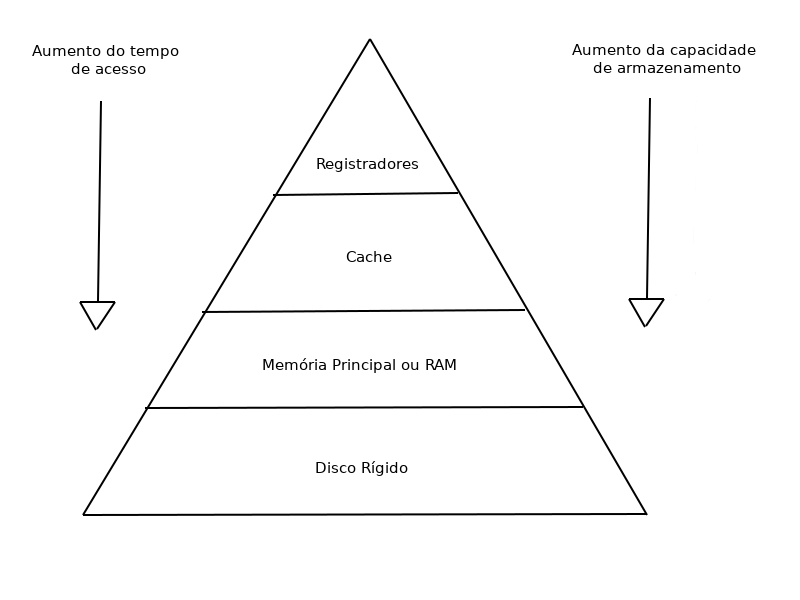
\includegraphics[width =.6\textwidth]{../figuras/memoryhierarchy}
    \par\medskip
    Fonte: Adaptado de~\cite{Toy1986}.
    \label{memhier}
\end{figure}

As camadas do sistema de mem�ria est�o descritas a seguir: 

\begin{itemize}
    \item Registradores: s�o as por��es da mem�ria com o acesso mais r�pido, por�m em 
        menor quantidade, com pouca capacidade de armazenamento e um alto custo de 
        fabrica��o, s�o localizados dentro do processador. Geralmente os programadores 
        n�o possuem controle sobre os registradores~\cite{Clements:2006:PCH:1214951}.
    \item Cache: localizado pr�ximo ao processador, fornece velocidade de acesso r�pida e armazena c�digo e dados utilizados 
        recentemente. Quando o processador tenta acessar algum dado presente no cache, ocorre um acerto do cache 
        (\textit{cache hit}), quando o dado n�o se encontra no cache, ocorre um erro do cache (\textit{cache miss}), e o dado 
        precisa ser buscado na mem�ria principal~\cite{Mahapatra:1999:PBP:357783.331677}.
    \item Mem�ria Principal, \textit{Dynamic Random Access Memory} (DRAM): em maior quantidade quando comparado ao cache,
        possui um custo menor, por�m com um tempo de acesso 
        maior, � respons�vel por lidar com as opera��es de entrada e sa�da. Apesar de ser muito mais lenta do que o cache, sua 
        estrutura simplificada e relativamente baixo custo fez com que a DRAM se tornasse a mem�ria principal dos sistemas 
        modernos~\cite{Mahapatra:1999:PBP:357783.331677}.
    \item Disco R�gido: possui a maior quantidade de armazenamento por�m a custo de um tempo de leitura substancialmente maior, 
        quando um programa � executado os seus dados s�o carregados para a mem�ria principal e a comunica��o com o disco r�gido 
        n�o � frequente, portanto essa unidade de mem�ria n�o ser� objeto de estudo deste trabalho.
\end{itemize}

Como citado anteriormente, os processadores obtiveram um enorme avan�o nos �ltimos tempos. Por�m, a mem�ria DRAM n�o foi 
capaz de acompanhar esse crescimento dos processadores na mesma velocidade. Desde a d�cada de 1980 at� a d�cada de 1990, os 
processadores t�m aprimorado a uma taxa de 60 porcento ao ano, enquanto que o tempo de acesso � DRAM tem aprimorado a uma 
taxa de menos de 10 porcento ao ano~\cite{Patterson:1997:CIR:623274.624083}. Mesmo com o r�pido crescimento tecnol�gico, essas 
estat�sticas de crescimento n�o sofreram altera��es nas d�cadas de 2000 e 2010.

Essa disparidade de crescimento tem aumentado a lacuna de desempenho entre processador-mem�ria, pois 
a lat�ncia de acesso a mem�ria pelo processador est� cada vez maior. Sempre que ocorre um \textit{cache miss}, o processador 
precisa ficar alguns ciclos ocioso enquanto aguarda o dado necess�rio ser buscado na mem�ria 
principal~\cite{Mahapatra:1999:PBP:357783.331677}, como a velocidade de 
acesso � mem�ria � relativamente muito menor do que a velocidade de processamento, um processador mais r�pido significa apenas 
mais ciclos ociosos. Isso � conhecido como "Gargalo do Processador-Mem�ria", e diante de tais limita��es f�sicas, surge a 
necessidade de boas pr�ticas de programa��o para que ocorra a menor quantidade poss�vel de \textit{cache misses}.

Com esse problema em mente, ao analisar o \textit{design} de programa��o orientada a 
objetos, percebe-se que essa abordagem, enquanto que mais leg�vel e com c�digo mais 
reutiliz�vel, sofre muitas vezes em termos de efici�ncia de mem�ria, pois seu 
\textit{design} � centrado em torno do problema e suas poss�veis solu��es, e n�o em torno 
dos dados. Ou seja, possui uma forte abstra��o dos dados por�m a custo do desempenho.

Quando uma classe de objetos possui dados, chamados de atributos, isto significa que essa classe est� fornecendo um contexto 
aos dados, e este pode comprometer o uso destes dados, pois ao adicionar m�todos ao contexto, pode-se criar a necessidade 
de adicionar mais dados � classe, o que pode rapidamente levar � classes que cont�m diversos fragmentos de dados que n�o 
est�o relacionados entre si~\cite{fabiandod}.

Outra desvantagem do uso demasiado de programa��o orientada a objetos, est� em sua pr�pria defini��o, que opera sobre um �nico 
objeto. Essa organiza��o de dados n�o � ben�fica ao processador, ao buscar objetos na mem�ria para se realizar opera��es sobre 
atributos espec�ficos destes, todos os outros dados pertencentes � classe tamb�m precisam ser carregados, deixando os caches 
polu�dos com dados desnecess�rios e aumentando a incoer�ncia de cache.

Com a premissa de amenizar o m�ximo poss�vel estes problemas, a modelagem orientada a 
dados (MOD), como o nome sugere, encoraja a mudan�a da perspectiva da programa��o dos 
objetos para os dados, seus tipos, como est�o armazenados na mem�ria e como ser�o lidos e 
processados~\cite{fabiandod}. Para alcan�ar esses objetivos, essa t�cnica sugere dividir 
cada objeto em diferentes componentes, e agrupar componentes do mesmo tipo na mem�ria, 
sem se importar de qual objeto vieram. Isso resulta em largos blocos de dados homog�neos, 
permitindo o processamento sequencial dos dados, e garantindo um aprimoramento 
significativo no desempenho~\cite{fabiandod}.

Esta abordagem de modelagem � mais condizente com a realidade de muitos programas complexos, pois raramente h� apenas um ou uma pequena 
quantidade de objetos de um determinado tipo, sendo necess�rio o processamento de todos eles. Mas esta abordagem n�o traz a 
solu��o para todos os problemas, e tamb�m possui suas desvantagens, sendo uma delas a falta de intuitividade para codifica��o 
orientada a dados. Uma das vantagens da orienta��o a objetos � a similaridade do pensamento com o mundo real e os seus 
problemas, deixando o c�digo mais leg�vel para os humanos. A modelagem orientada a dados 
requer um racioc�cio menos natural comparado � modelagem orientada a objetos, tornando 
por vezes o c�digo menos intuitivo.

Para as aplica��es na �rea de computa��o gr�fica, esses problemas n�o seriam diferentes, principalmente levando em 
considera��o que uma grande parte dos trabalhos nessa �rea utilizam a programa��o orientada a objetos. Essas aplica��es, 
principalmente jogos eletr�nicos modernos, utilizam um complexo sistema o qual possui muitos componentes diferentes que 
cont�m dados que constantemente transitam entre a mem�ria, o processador e a GPU. Esse sistema � comumente conhecido 
como motor de jogos (do ingl�s \textit{Game Engine}), ou simplesmente como \textit{engine}.

Um motor de jogos, apesar de n�o possuir uma defini��o absoluta, � geralmente entendida como o software respons�vel por lidar com 
todos os m�dulos que juntos comp�em um jogo eletr�nico, como por exemplo, bibliotecas matem�ticas (contendo opera��es de vetores, 
matrizes, quaternions, m�todos trigonom�tricos, etc.), ger�ncia de mem�ria, 
estruturas de dados personalizadas, o motor de renderiza��o, gerenciador de recursos, ferramentas para depura��o e an�lise de desempenho, sistemas 
de colis�o e f�sica, sistema de anima��es e part�culas, sistema de detec��o de inputs (mouse, teclado e outros controladores),
sistema de �udio, sistema de rede para jogos online, entre outros~\cite{gregory2009game}.

Para complementar, um motor de jogos pode ser entendido como um conjunto de bibliotecas e ferramentas, os quais combinados 
s�o respons�veis por administrar toda a parte l�gica de uma aplica��o gr�fica. O motor � separado em diferentes componentes, 
que s�o conhecidos como componentes n�cleo, estes fornecem utilidades que aceleram o processo de desenvolvimento 
das aplica��es. A introdu��o dos motores de jogos na ind�stria de jogos digitais tamb�m introduziu um novo paradigma, 
uma nova maneira de desenvolver jogos, na qual � feita uma completa e clara separa��o do conte�do l�gico e do conte�do criativo (arte, 
anima��es, m�sica, sons, texturas, etc.).

O motor de renderiza��o, tamb�m conhecido como motor gr�fico, � um dos maiores e mais complexos componentes de um motor de 
jogos. E apesar de n�o possuir apenas uma �nica maneira de projet�-los, a maioria dos motores de renderiza��o modernos 
seguem filosofias de \textit{design} em comum~\cite{gregory2009game}. Esse componente ser� respons�vel por todos os m�todos, 
estruturas e otimiza��es que ser�o respons�veis pela renderiza��o dos gr�ficos e anima��es do jogo. 

Um dos elementos 
presentes no motor gr�fico � uma interface de dispositivo gr�ficos, que ser� respons�vel pela comunica��o com a GPU 
e, consequentemente, com a renderiza��o de baixo n�vel. Uma das bibliotecas capazes de realizar essa fun��o � o OpenGL, uma 
API gr�fica para acessar os recursos da GPU, contendo um rico conjunto de comandos (mais de 500) que s�o utilizados para 
especificar objetos, imagens e opera��es necess�rias para a renderiza��o de aplica��es gr�ficas~\cite{shreiner2013opengl}.
Existem outras alternativas ao OpenGL que tamb�m s�o populares no mercado, como por 
exemplo o DirectX, desenvolvido pela Microsoft\textit{https://www.microsoft.com} e que ao 
longo dos anos foi tamb�m foi projetado para oferecer uma vasta gama de 
funcionalidades~\cite{zink2016practical}.

A programa��o em OpenGL moderno tamb�m requer o uso e entendimento de outro conceito 
igualmente importante, os \textit{shaders}, que s�o pequenos programas que s�o 
especialmente compilados para a GPU e suas instru��es s�o executadas diretamente 
nos n�cleos da GPU~\cite{shreiner2013opengl}. Shaders em OpenGL utilizam uma linguagem de 
programa��o pr�pria, o GLSL (\textit{OpenGL Shading Language})~\cite{shreiner2013opengl}.

Al�m dessa camada de renderiza��o de baixo n�vel, o motor gr�fico tamb�m conta com componentes essenciais de mais alto n�vel 
que s�o respons�veis pela ger�ncia da geometria das malhas, como um grafo de cenas, que al�m de manipular as malhas estabelece 
a hierarquia entre elas e define subdivis�es espaciais~\cite{gregory2009game}. T�cnicas de otimiza��es tamb�m s�o importantes, 
como por exemplo a remo��o parcial de objetos que n�o s�o considerados para contribuir � imagem final, essa t�cnica � 
conhecida como \textit{culling}~\cite{akenine2008real}.

Todos esses elementos, t�cnicas e otimiza��es do motor gr�fico no fim constroem o que � 
conhecido como \textit{pipeline} de renderiza��o. A principal fun��o desse 
\textit{pipeline} � renderizar uma imagem bidimensional, dada uma c�mera virtual, objetos 
tridimensionais, fontes de luz, equa��es de sombreamento, texturas, entre 
outros~\cite{akenine2008real}.

Considerando os problemas supracitados a respeito do gargalo de desempenho do processador-mem�ria, e das desvantagens da 
programa��o orientada a objetos, este trabalho prop�e a implementa��o de um motor de jogos desde o princ�pio com o objetivo de 
explorar o potencial da modelagem orientada a dados, um conceito pouco difundido entre a comunidade de programadores, 
e seus benef�cios para aplica��es gr�ficas, uma �rea na qual a orienta��o a objetos est� fortemente impregnada. Uma vez
que um motor de jogos completo � uma aplica��o consideravelmente grande e complexa, neste trabalho concentrou-se na implementa��o
do motor gr�fico e suas otimiza��es.

\section{Objetivos}
\label{obj}

\textbf{Objetivo geral}: Investigar o potencial da modelagem orientada a dados para o 
desenvolvimento de um motor de jogos e analisar sua efici�ncia e desempenho.\\

\noindent\textbf{Objetivos espec�ficos}: 
Abaixo encontra-se uma lista dos principais objetivos a serem alcan�ados com este trabalho.
\begin{itemize}
    \item Verificar o estado atual no que diz respeito �s implementa��es de motores de jogos modernos;
    \item Utilizar o conceito de \textit{design} orientado a dados para proporcionar uma melhora
        no desempenho dos motores gr�ficos atrav�s da coer�ncia de cache.
    \item Analisar o desempenho do motor de jogos, atrav�s do desenvolvimento de uma 
        aplica��o que utilize suas funcionalidades em duas vers�es, uma orientada a 
        objetos e outra orientada a dados, comparando essas duas vers�es.
    \item Demonstrar as mudan�as necess�rias para converter uma aplica��o orientada a 
        objetos para uma aplica��o orientada a dados.
\end{itemize}

%------------------------------------------------
\section{Metodologia}
\label{met}

Ap�s a etapa de revis�o bibliogr�fica sobre os conceitos necess�rios para 
a implementa��o do motor de jogos, a aplica��o foi desenvolvida em etapas 
e o m�todo utilizado foi a implementa��o dos componentes do motor sequencialmente, 
no qual estes ser�o testados individualmente.

A etapa seguinte foi a integra��o dos componentes para a constru��o de um motor de 
jogos utilizando programa��o orientada a objetos. Com o motor de jogos tendo todos 
os seus componentes e caracter�sticas funcionando devidamente, uma segunda vers�o 
do motor de jogos foi desenvolvida, utilizando os conceitos estudados da modelagem 
orientada a dados. Com as duas vers�es implementadas, foram feitas an�lises e compara��es 
do desempenho e efici�ncia das duas vers�es.

\section{Organiza��o do Trabalho}
\label{paperstructure}

Este trabalho est� organizado da seguinte forma, no Cap�tulo 2 est�o contidos os 
fundamentos para o desenvolvimento do trabalho, o Cap�tulo 3 detalha alguns trabalhos 
relacionados com o tema deste projeto, j� o Cap�tulo 4 apresenta o projeto dos motores 
desenvolvidos e as diferen�as entre os dois. No cap�tulo~\ref{resultscap} est�o os resultados 
de desempenho e compara��es entre as duas abordagens e por fim, no Cap�tulo 6 est�o contidas 
as considera��es finais, seguidas pelas refer�ncias bibliogr�ficas.

\setlength\abovedisplayskip{0pt} \setlength\belowdisplayskip{0pt}
\setlength\abovedisplayshortskip{0pt} \setlength\belowdisplayshortskip{0pt}

\chapter{Fundamenta\c{c}\~ao Te\'orica}
\label{theorycap}

Neste cap�tulo ser�o discutidos e explicados todos os conceitos e 
fundamentos necess�rios para a compreens�o da proposta 
feita nesse trabalho, assim como a abordagem que ser� utilizada 
para a implementa��o de todos os componentes que juntos v�o compor 
o motor de jogos que ser� o objeto de estudo.

\section{Modelagem Orientada a Dados}
\label{secdataorienteddesign}

A modelagem orientada a dados (do ingl�s: \textit{Data Oriented Design}) � 
uma forma de codificar os programas que prop�e uma mudan�a no foco da 
implementa��o: ao inv�s de se focar no c�digo, o foco deve estar nos 
dados. Apesar do termo "orienta��o a dados"\ ter sido usado apenas recentemente, 
a utiliza��o dos conceitos dessa t�cnica j� t�m sido usados h� muito mais tempo 
do que a introdu��o do termo.

Orienta��o a dados foi introduzido por John A. Sharp~\cite{Sharp1980}, cujo objetivo 
era aumentar a efici�ncia do processador e da utiliza��o da mem�ria. Al�m disso, o autor 
cita que um dos objetivos dessa t�cnica de programa��o � facilitar a concorr�ncia na 
execu��o dos programas. No seu trabalho � proposta uma metodologia de projeto que 
menciona outro conceito importante, o do fluxo de dados.

Ao se projetar um programa ou sistema, a primeira tarefa a ser feita � determinar o 
fluxo de dados necess�rios. Essa etapa consiste em determinar quais componentes do 
sistema requerem cada um dos diferentes tipos de dados presente neste, e tamb�m 
especificar quais s�o os componentes que geram novos dados. Depois que o fluxo de dados 
no sistema est� completamente especificado, o pr�ximo passo � descrever como os dados 
recebidos por cada componente s�o transformados nos dados que este componente precisa 
gerar. Sharp defende que qualquer programa pode ser descrito dessa maneira, a 
transforma��o de um dado conjunto de \textit{inputs} para um certo conjunto de 
\textit{outputs} requeridos.

Um exemplo � o trabalho de Chellappa et al.~\cite{chellappa2008write}, no 
qual � reconhecido o problema da velocidade de acesso � mem�ria principal pelo 
processador, e para solucionar esse problema � dito que os dados de uma aplica��o devem 
ser lidos na ordem apropriada. Otimiza��es feitas pelos compiladores s�o 
limitadas para o caso da leitura da mem�ria, para realizar esse tipo de 
otimiza��o seria necess�rio conhecimento do dom�nio do problema e dos algoritmos 
utilizados, algo que os compiladores n�o possuem. 

Al�m disso � reconhecido pelos autores o fato de um \textit{cache miss} causar a perda de 
ciclos e, consequentemente, a perda de opera��es de ponto flutuante. Para demonstra��o do 
problema e sua solu��o atrav�s da reestrutura��o de c�digo, s�o mostrados no artigo 
dois algoritmos diferentes. Um deles � de particular interesse para esse trabalho, que 
� a multiplica��o entre matrizes pois conforme visto na se��o~\ref{secmathconcepts}, 
opera��es de �lgebra linear s�o extensivamente utilizadas em aplica��es gr�ficas.

Como as otimiza��es feitas pelo compilador s�o limitadas, � necess�rio estruturar o 
c�digo de maneira inteligente para que o acesso � mem�ria seja o menos frequente  
poss�vel e para aprimorar a coer�ncia de cache, e � para esse aspecto que a MOD serve.
Um dos objetivos dessa t�cnica � permitir a leitura sequencial dos dados. Para atingir 
isso, os objetos pertencentes ao dom�nio do problema s�o representados por 
identificadores �nicos que s�o utilizados para acessar suas propriedades. Essas 
propriedades s�o \textit{arrays} de dados que s�o armazenados na mem�ria de maneira 
cont�gua, e para utilizar essa t�cnica de maneira eficiente, � essencial administrar 
esses \textit{arrays} das propriedades para garantir que permane�am cont�guos conforme 
novos dados s�o adicionados e removidos~\cite{Fontana2017}.

Ao se modelar o c�digo atrav�s de uma abordagem orientada a objetos, esta modelagem 
� centrada em volta do problema e da sua solu��o. Os objetos, que n�o s�o coisas reais, 
mas sim o resultado das solu��es para o problema apresentado, manipulam apenas os dados 
necess�rios para represent�-los sem nenhuma considera��o pelo hardware, pelos 
padr�es de dados reais ou de quantidades, por isso essa abordagem permite uma r�pida 
prototipagem dos programas pois essas solu��es podem ser escritas diretamente da 
modelagem para o c�digo~\cite{fabiandod}.

A MOD utiliza uma abordagem diferente, prevendo onde os dados s�o mais vistos ou 
esperados atrav�s da determina��o do fluxo de dados, utiliza o caso 
mais prov�vel para direcionar a escolha do algoritmo. Com isso, ao se utilizar essa 
abordagem pode-se separar os dados mais utilizados dos menos utilizados de tal forma 
que estes n�o sejam desnecessariamente carregados da mem�ria. N�o 
saber como esses dados est�o armazenados na mem�ria pode ser 
prejudicial para o desempenho do programa.

\begin{figure}[h]
    \centering
    \captionof{figure}{Orienta��o a objetos vs. Orienta��o a Dados. Duas maneiras 
    diferentes de se ler os dados da mem�ria.}
    \begin{subfigure}[b]{0.35\textwidth}
        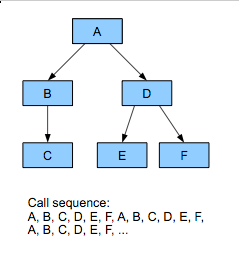
\includegraphics[width=\textwidth]{../figuras/objectreadingorder}
        \caption{Orienta��o a Objetos}
        \label{fig:ood}
    \end{subfigure}
    \begin{subfigure}[b]{0.35\textwidth}
        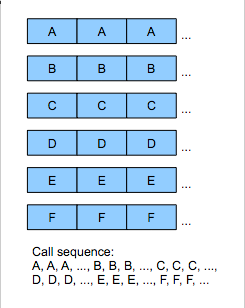
\includegraphics[width=\textwidth]{../figuras/dodreadingorder}
        \caption{Orienta��o a Dados}
        \label{fig:dod}
    \end{subfigure}
    \par\medskip
    Adaptado de: <http://gamesfromwithin.com/data-oriented-design>. Acesso em: 27/05/2017.
    \label{oodvsdod}
\end{figure}

\medskip

A figura~\ref{oodvsdod} apresenta duas maneiras diferentes de se ler dados da mem�ria, 
a primeira ocorre com a programa��o orientada a objetos, na qual os dados n�o s�o lidos 
de maneira cont�gua, a sequ�ncia de chamadas da figura ocorre para todos os objetos 
caso uma fun��o ou uma rotina chame todos os objetos daquele tipo, o que n�o � uma 
situa��o incomum de se acontecer. � preciso passar por todas as refer�ncias caso seja 
necess�rio acessar os dados nos n�veis mais baixos da �rvore, e se uma fun��o usar
somente alguns desses elementos, essa leitura de dados n�o � muito eficiente. 

Na figura~\ref{fig:dod} h� uma separa��o do objeto em componentes diferentes, e 
componentes do mesmo tipo s�o agrupados juntos na mem�ria, independentemente do objeto 
de qual vieram. Essa organiza��o resulta em blocos largos de dados homog�neos, 
permitindo o uso eficiente de mem�ria atrav�s processamento de dados cont�guos. 

Outra proposta da MOD, al�m da divis�o dos objetos em diferentes 
componentes, � utilizar a ordena��o de dados ao inv�s de armazenar 
o estado de um objeto. O motivo de evitar o armazenamento do estado 
de um objeto se deve pela necessidade de condicionais para checar 
esse estado.

O uso de condicionais dentro de um \textit{loop} pode causar 
\textit{branching}, que � o ato da troca da atual sequ�ncia de 
instru��es do programa por uma outra sequ�ncia, caracterizando um 
desvio do comportamento padr�o de execu��o das instru��es em 
ordem~\cite{knuthart}. Tal desvio � causado pela execu��o de uma instru��o que 
causa ramifica��o na execu��o do programa, instru��es com condicionais 
s�o exemplos de instru��es que causam \textit{branching}.

O \textit{branching} � um dos fatores que dificultam o uso de uma t�cnica conhecida 
por cache \textit{prefetching}, utilizada pelos processadores para aprimorar o 
desempenho, algumas instru��es ou dados s�o buscados da mem�ria principal e movidos 
para o cache antes que seja necess�rio us�-los~\cite{smith1982}. Para que o 
\textit{prefetching} ocorra, � necess�rio que o algoritmo respons�vel pela 
t�cnica preveja qual ramo ser� o executado. Caso a escolha esteja errada, 
o erro de previs�o causa penalidades no desempenho, e o processador precisa 
despejar as instru��es ou dados que haviam sido buscadas de 
antem�o~\cite{tianprefetch}.

Se uma refer�ncia a um \textit{array} � precedida por uma instru��o com 
condicionais, h� dois problemas para se realizar o \textit{prefetching} dos 
dados do \textit{array}: o primeiro problema � que o teste condicional da 
instru��o pode ser verdadeiro somente para um subconjunto do \textit{array} 
e realizar um \textit{prefetching} no \textit{array} poderia resultar na 
transfer�ncia desnecess�rias de dados para o cache. O segundo problema � 
que o teste condicional pode estar impedindo o referenciamento de dados 
n�o existentes no \textit{array}, e realizar o \textit{prefetching} para 
esses dados poderia resultar em comportamento 
inesperado~\cite{vanderwieldataprefetch}.

Para evitar o uso de instru��es com condicionais, principalmente em 
m�todos que s�o utilizados com frequ�ncia, pode-se separar os dados entre 
aqueles que passam no teste condicional e aqueles que n�o passam, desta 
forma a verifica��o com condicionais se torna desnecess�ria, e o fluxo de 
execu��o das instru��es n�o � interrompido por \textit{branching}.

O desvio excessivo da ordem de execu��o padr�o de um programa 
tamb�m pode ser evitado tratando sempre o caso mais comum primeiro.
 Isso significa que, ao descrever uma transforma��o sobre um 
\textit{input} de dados, essa transforma��o deve levar em 
considera��o qual ser� o caso mais comum para esse \textit{input}, 
em termos de estado e de quantidade. 

Em aplica��es desenvolvidas com programa��o orientada a objetos, 
as transforma��es de dados geralmente s�o feitas atrav�s dos 
m�todos implementados de cada classe. Esses m�todos est�o no 
escopo do objeto e por isso n�o possuem acesso aos atributos dos 
outros objetos da mesma classe. Consequentemente as instru��es 
descritas nos m�todos operam somente sobre os atributos do objeto 
que fez a chamada do m�todo.

Essa abordagem � irrealista no contexto de jogos e aplica��es 
gr�ficas, pois em poucas situa��es o caso mais comum ser� um 
�nico objeto. Se o caso mais
comum de \textit{input} para uma transforma��o � um conjunto 
de objetos, ent�o essa transforma��o 
deve conter instru��es que operam sobre o conjunto inteiro de 
objetos e somente sobre as propriedades que s�o realmente 
necess�rias, otimizando o fluxo de instru��es e o acesso � 
mem�ria~\cite{fabiandod}. Transforma��es sobre um �nico objeto 
causam polui��o desnecess�ria do cache quando estas precisam 
ser feitas sobre v�rios objetos em sequ�ncia, principalmente 
quando somente uma parcela dos atributos do objeto � 
necess�ria.

O esquema de armazenamento apresentado na 
figura~\ref{fig:dod} � um meio de se armazenar uma sequ�ncia de 
dados na mem�ria conhecido como \textit{Structure of Arrays} (SoA), 
no qual os dados de um registro s�o separados em \textit{arrays} 
paralelos, um para cada atributo do registro. Desta maneira, uma 
estrutura armazena os dados de todos os registros, em contraste 
com a outra abordagem apresentada na figura~\ref{fig:ood} conhecida 
como \textit{Array of Structures} (AoS), no qual o armazenamento 
dos dados dos registros � feito de maneira intercalada (todas 
as propriedades do registro s�o alocadas sequencialmente na mem�ria).
Uma lista de objetos � um exemplo de AoS.

� relevante observar que n�o h� uma abordagem melhor para todos os 
casos. As duas abordagens possuem suas vantagens e desvantagens, 
cabe ao desenvolvedor ter o conhecimento sobre o uso dos dados 
para determinar qual abordagem dever� ser utilizada. Quanto menos 
propriedades de um objeto forem necess�rias para uma certa 
transforma��o de dados, mais eficiente o SoA se torna para essa 
transforma��o, caso contr�rio, o AoS pode ser uma abordagem mais 
apropriada.

O SoA � mais eficiente para transforma��es com poucas propriedades 
pois ao se mover os dados da mem�ria ao cache, este ser� menos 
polu�do com dados n�o relacionados caso a estrutura possua 
muitas propriedades n�o necess�rias para a transforma��o. 
Caso muitas propriedades sejam necess�rias para uma transforma��o, 
a SoA se torna menos eficiente, pois as propriedades dos objetos 
estar�o alocadas mais distantes uma da outra, tornando o acesso 
aos dados mais lento~\cite{Fontana2017}.

\section{Motor de Jogos}
\label{secgameengine}

O termo e o conceito de motor de jogos surgiram no in�cio da d�cada de 1990, quando a 
empresa \textit{Id Software} lan�ou o jogo \textit{DOOM} e, juntamente com ele, seu 
motor de jogos conhecido como \textit{DOOM Engine}, que depois foi nomeado como 
\textit{Id Tech 1}~\cite{gregory2009game}.
O jogo \textit{DOOM}, atrav�s da \textit{Id Tech 1}, � considerado o primeiro jogo da 
ind�stria de jogos digitais que possui uma clara separa��o entre os componentes n�cleo 
do jogo, chamada de parte l�gica, dos componentes criativos, tais como anima��es, 
modelos geom�tricos, sons, imagens, planos de fundo, m�sica, etc.
A \textit{Id Software}, al�m de ter criado um novo conceito de \textit{software} 
na ind�stria de jogos que atualmente � considerado padr�o em grandes empresas e ter 
gerado uma vasta fam�lia de motores de jogos que partiram da \textit{Id Tech 1}, tamb�m 
conceberam um novo paradigma para se desenvolver jogos digitais.

A maior vantagem da utiliza��o de motores de jogos consiste na reutiliza��o de c�digo. 
Isso significa que, para rotinas parecidas, ou at� mesmo para outros projetos, um mesmo 
c�digo pode ser utilizado mudando-se apenas alguns par�metros. Al�m disso, um motor de 
jogos mais completo geralmente permite uma r�pida prototipagem de novos projetos,
requer uma habilidade menor por parte dos programadores e minimiza seus esfor�os 
atrav�s de abstra��es.

A implementa��o de um motor de jogos � feita atrav�s do desenvolvimento separado de 
diversos componentes. Cada componente � respons�vel por uma parte espec�fica da parte 
l�gica do jogo, o oposto do que era feito na programa��o tradicional de jogos, cujo 
objetivo prim�rio era maximizar o desempenho para o hardware utilizado. Essa preocupa��o 
com o desempenho, juntamente com o curto intervalo de tempo que os desenvolvedores tinham 
para terminar os projetos geralmente resultava em c�digos que n�o ficavam conforme os 
preceitos de boa engenharia de software segundo Kruchten et al.~\cite{Kruchten2006}.

Dada a complexidade que � desenvolver um motor de jogos, considerando todos os aspectos que 
este deve abranger, desenvolver um c�digo monol�tico sem estrutura arquitetural e sem se 
preocupar com o design geral do sistema, implica em um \textit{software} cujos componentes 
s�o todos dependentes entre si. O resultado dessa depend�ncia � um sistema fr�gil, no qual 
pequenas mudan�as em alguma parte do c�digo pode afetar outras partes de maneiras n�o 
�bvias, al�m de desencorajar os programadores a alterar o c�digo ou refator�-lo para 
aumentar sua qualidade~\cite{Keenan2011}.

Por esse motivo, � importante que um motor de jogos esteja devidamente modularizado para 
evitar um sistema fr�gil, e facilitar a adi��o de novos componentes. � importante lembrar 
que, apesar de ser desej�vel que os componentes estejam o mais independentes o poss�vel 
entre si, estes devem estar funcionando perfeitamente em sinergia, isto �, um motor de 
jogos n�o funciona com v�rios componentes executando separadamente, mas sim com a 
comunica��o entre eles de maneira clara e eficiente.

A comunica��o e integra��o entre os diferentes componentes de um motor de jogos faz parte 
da modelagem da arquitetura deste. Conforme apontado por Anderson et 
al.~\cite{Anderson2008}, um problema que ainda persiste atualmente � a falta de material 
na literatura a respeito da modelagem da arquitetura de motores de jogos, sendo que a 
maior parte da pesquisa dispon�vel foca somente nos componentes separados, como 
renderiza��o, intelig�ncia artificial (IA) ou rede. Ainda � salientado pelo autor que 
n�o h� um consenso sobre os limites que separam um jogo do seu motor, portanto 
h� espa�o a ser explorado nessa �rea.

A quantidade de componentes presentes em um motor de jogos � altamente dependente da 
complexidade desejada para o jogo sendo desenvolvido, alguns dos componentes mais 
presentes s�o: componente gr�fico, colis�es, f�sica, intelig�ncia artificial, rede, som 
e anima��o.

\section{Conceitos Matem�ticos}
\label{secmathconcepts}

Qualquer motor de jogos necessita de uma biblioteca matem�tica, uma vez que 
jogos s�o aplica��es as quais s�o extremamente dependentes de opera��es e 
conceitos matem�ticos. 
Essas bibliotecas fornecem diversas utilidades, algoritmos e fun��es 
matem�ticas, tais como: estruturas de dados personalizadas de vetores, 
matrizes e quaternions; opera��es matriciais e vetoriais; rota��es e 
interpola��es de quaternions; trigonometria; opera��es geom�tricas com 
linhas, raios, esferas, etc., manipula��o de \textit{splines}, integra��o 
num�rica, e quaisquer outras utilidades que os desenvolvedores 
necessitarem~\cite{gregory2009game}.

A �rea da computa��o gr�fica est� intimamente ligada �s �reas da matem�tica de 
�lgebra linear e geometria anal�tica, a maior parte dos conceitos matem�ticos empregados 
neste trabalho pertencem a uma destas �reas. Visto que ambas estas �reas s�o vastas e v�o 
muito al�m do escopo deste trabalho, o restante desta se��o tratar� dos conceitos e 
propriedades que s�o relevantes para a computa��o gr�fica apenas.

Verth e Bishop~\cite{Verth:2008} e Mortenson~\cite{mortenson1999mathematics} fizeram uma 
cobertura de toda a matem�tica essencial utilizada em motores de jogos. O restante 
da se��o cobrir� apenas os t�picos essenciais e para uma abordagem mais completa do 
assunto, esses trabalhos dever�o ser consultados. Todos os conceitos apresentados aqui 
s�o utilizados para a elabora��o da biblioteca matem�tica presente neste trabalho.

\subsection{Vetores e Pontos}

Vetores e pontos s�o as estruturas essenciais de todos os objetos presentes em 
aplica��es gr�ficas. 
Os pontos representam posi��es do espa�o e podem ser utilizados para determinar os 
v�rtices da superf�cie de um objeto, que consequentemente determinar� seu formato 
(chamado de modelo). Os pontos tamb�m podem representar a posi��o de um objeto no 
espa�o, a qual geralmente se refere ao centro do objeto. Se os pontos de um objeto 
forem alterados, o modelo desse objeto tamb�m ser� alterado.

Vetores (no campo da geometria) s�o entidades que possuem uma dire��o, um comprimento, 
chamado de magnitude, e um sentido (por exemplo, da esquerda para direita ou de baixo 
para cima), os vetores representam a diferen�a entre dois pontos. S�o utilizados para 
armazenar grandezas (como velocidade, gravidade, acelera��o, atrito, etc.) e dire��es.
H� alguns casos espec�ficos de vetores que recebem nomea��es 
diferentes, por exemplo vetores cuja magnitude � igual a 1 s�o chamados de vetores 
unit�rios ou vetores normalizados. Um vetor cuja magnitude � igual a 0 � chamado de 
vetor zero, e n�o possui nenhuma dire��o. 

Para representar um vetor no computador, utiliza-se a chamada "base Euclidiana padr�o", 
composta pelos tr�s vetores unit�rios linearmente independentes $i$, $j$ e $k$ que s�o 
perpendiculares entre si para o caso do espa�o tridimensional $\mathbb{R}^3$. Para o 
espa�o bidimensional $\mathbb{R}^2$, utiliza-se somente os vetores $i$ e $j$. 

Utilizando essa base, pode-se representar unicamente qualquer vetor no espa�o atrav�s 
de uma combina��o linear dos tr�s vetores base da seguinte maneira: 

\begin{equation}
    \centering
    v = xi + yj + zk
\end{equation}

Os coeficientes $x$, $y$ e $z$ representam o deslocamento em cada um dos eixos. A 
figura~\ref{3dbasisvector} demonstra como um vetor � representado utilizando a base 
Euclidiana padr�o. Esses coeficientes s�o utilizados para representar um vetor 
algebricamente atrav�s de uma tripla $(x,y,z)$, ou uma dupla para o caso dos vetores 
2D, e s�o conhecidos como componentes do vetor.

\begin{figure}[h]
    \centering
    \captionof{figure}{Representa��o de um Vetor na Base Tridimensional.}
    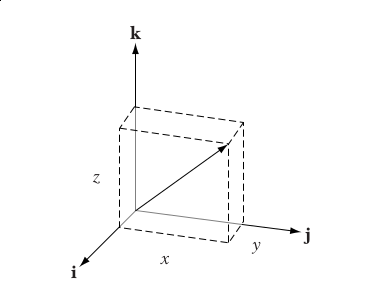
\includegraphics[width =.6\textwidth]{../figuras/3dbasisvector}
    \par\medskip
    Fonte: \cite{Verth:2008}.
    \label{3dbasisvector}
\end{figure}

Com essa representa��o alg�brica, pode-se definir as opera��es sobre vetores t�o 
utilizadas na computa��o gr�fica.

\subsection{Opera��es Sobre Vetores}

Nesta se��o ser�o apresentadas opera��es que podem ser feitas sobre vetores e entre 
vetores. Para todas as opera��es ser�o utilizados como exemplo vetores no espa�o 3D.
\subsubsection{Adi��o}

A adi��o entre dois vetores � feita atrav�s da soma de cada um dos componentes de um 
vetor com os componentes correspondentes do outro vetor.

\begin{equation}
    \begin{aligned}
        v1 + v2 = (x_1, y_1, z_1) + (x_2, y_2, z_2) \\
        v1 + v2 = (x_1 + x_2, y_1 + y_2 , z_1 + z_2)
    \end{aligned}
\end{equation}

\subsubsection{Subtra��o}

A subtra��o entre dois vetores � semelhante � adi��o, por�m s�o feitas opera��es de 
substra��es entre os componentes dos operandos.

\begin{equation}
    \begin{aligned}
        v1 - v2 = (x_1, y_1, z_1) - (x_2, y_2, z_2) \\
        v1 - v2 = (x_1 - x_2, y_1 - y_2, z_1 - z_2)
    \end{aligned}
\end{equation}

Observa-se que assim como a subtra��o entre escalares, a subtra��o entre vetores tamb�m 
n�o � comutativa.

\subsubsection{Multiplica��o por Escalar}

Dado um certo coeficiente $k$, a multiplica��o de um vetor $v$ pelo escalar $k$ � dada 
pela multiplica��o do escalar por cada um dos componentes do vetor:

\begin{equation}
    \begin{aligned}
        kv = k(x, y, z)\\
        kv = (kx, ky, kz)
    \end{aligned}
\end{equation}

\subsubsection{Igualdade Entre Vetores}

Um vetor $v1$ � igual a um vetor $v2$, se todos os componentes de $v1$ forem iguais aos 
componentes correspondentes de $v2$. 

\begin{equation}
    \begin{aligned}
        v1 = v2\\
        (x_1, y_1, z_1) = (x_2, y_2, z_2)\\
        x_1 = x_2, y_1 = y_2, z_1 = z_2
    \end{aligned}
\end{equation}

\subsubsection{Magnitude}

O operador de magnitude serve para calcular o comprimento de um vetor. Para o faz�-lo, 
a norma utilizada � a norma Euclidiana, cujo c�lculo consiste na raiz quadrada da soma  
dos quadrados dos componentes. O operador de norma � denotado por: $||v||$. Dado um 
vetor $v$, o tamanho do vetor $d$ � dado por:

\begin{equation}
    \begin{aligned}
        ||v|| = d = \sqrt{x^2 + y^2 + z^2}
    \end{aligned}
\end{equation}

\subsubsection{Normaliza��o}

A normaliza��o de um vetor cria um vetor unit�rio $v'$ a partir de um vetor $v$, 
mudando sua magnitude para 1, por�m mantendo sua dire��o. Isso � feito a partir da
divis�o de um vetor pela sua norma:

\begin{equation}
    \begin{aligned}
        v' = \frac{v}{||v||}
    \end{aligned}
\end{equation}

\subsubsection{Produto Escalar}

O produto escalar entre dois vetores, como o nome sugere, resulta em um escalar a partir 
dos operandos, a opera��o � feita multiplicando-se os dois vetores 
componente-a-componente e depois somando os resultados:

\begin{equation}
    \begin{aligned}
        v1 \cdotp v2 = v1_xv2_x + v1_yv2_y + v1_zv2_z
    \end{aligned}
\end{equation}

Se os vetores $v1$ e $v2$ formarem um �ngulo de 90 graus entre si, ent�o o produto 
escalar entre eles ser� zero. Ent�o pode-se dizer que dois vetores ser�o 
perpendiculares, ou ortogonais, quando $v1 \cdotp v2 = 0$.

Al�m de verificar a ortogonalidade entre dois vetores, o produto escalar pode fornecer 
outras informa��es, por exemplo, se $v1 \cdotp v2 > 0$, ent�o o �ngulo entre eles � 
menor do que 90 graus, se $v1 \cdotp v2 < 0$, ent�o o �ngulo entre eles � maior do que 
90 graus, esse teste n�o requer que os vetores estejam normalizados.

\subsubsection{Produto Vetorial}

O produto vetorial, opostamente ao produto escalar, tem como resultado da opera��o um 
vetor. O vetor resultante $w$ do produto vetorial entre $v1$ e $v2$ ser� sempre 
ortogonal a estes. Como essa opera��o n�o � comutativa, a dire��o do vetor resultante 
depender� da ordem dos operandos, ou seja, h� duas sa�das poss�veis dessa opera��o, uma 
� a nega��o da outra. O produto vetorial � determinado pela f�rmula:

\begin{equation}
    \begin{aligned}
        v1 \times v2 = (v1_yv2_z - v2_yv1_z, v1_zv2_x - v2_zv1_x, v1_xv2_y - v2_xv1_y)
    \end{aligned}
\end{equation}

A figura~\ref{piccrossproduct} demonstra geometricamente um produto vetorial. Os usos mais 
comuns para o produto vetorial � para gerar um vetor ortogonal a outros dois e para 
verificar se dois vetores s�o paralelos entre si.

Diferentemente do produto escalar, o produto vetorial n�o � definido para vetores 2D.

\begin{figure}[h]
    \centering
    \captionof{figure}{Produto vetorial com os dois poss�veis resultados representados.}
    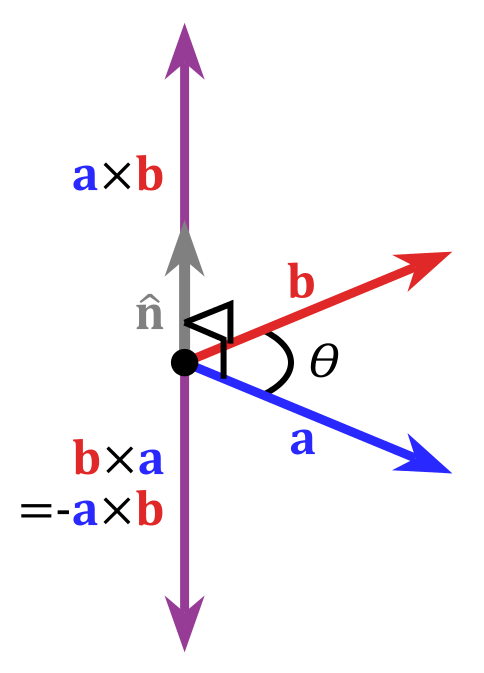
\includegraphics[width =.4\textwidth]{../figuras/crossproduct}
    \par\medskip
    Dispon�vel em: <https://en.wikipedia.org/wiki/Cross\_product>. Acesso em: 27/05/2017.
    \label{piccrossproduct}
\end{figure}

\subsection{Matrizes}
\label{matrices}

Matrizes s�o \textit{arrays} bidimensionais nas quais cada valor individual � chamado de 
elemento. A descri��o de uma matriz � feita especificando o seu n�mero de linhas e n�mero 
de colunas, sendo $m$ o n�mero de linhas e $n$ o n�mero de colunas, � dito que � uma matriz 
$m$ por $n$, denotado por $m\ \times n$. A rela��o da quantidade de linhas e colunas � 
tamb�m conhecida como o tamanho da matriz.

Uma linha � uma sequ�ncia de elementos na horizontal da esquerda para a direita, enquanto 
que uma coluna � uma sequ�ncia de elementos na vertical de cima para baixo. Para 
referenciar um elemento espec�fico de uma matriz $A$, usa-se a nota��o: $a_{i,j}$, onde 
$i$ referencia uma linha e $j$ uma coluna. Dessa maneira, o elemento $a_{1,2}$ � o elemento 
que est� na primeira linha e na segunda coluna na matriz A.
O conjunto de elementos os quais o n�mero da linha � igual ao n�mero da coluna (ex: 
$a_{1,1}$) � chamado de diagonal principal.

Alguns casos espec�ficos de matrizes recebem denota��es especiais. A seguir ser�o 
listadas algumas dessas matrizes espec�ficas:
\begin{itemize}
    \item Matriz quadrada: matriz cujo n�mero de linhas � igual ao n�mero de colunas 
    \item Matriz zero ou nula: matriz na qual todos os elementos s�o iguais a zero
    \item Matriz diagonal: matriz cujos �nicos elementos que n�o s�o zero s�o os da 
        diagonal principal
    \item Matriz Identidade: matriz na qual todos os elementos da diagonal principal s�o 
        iguais a um, e o restante igual a zero. A matriz identidade � denotada por $I$.
    \item Matriz coluna: matriz que s� possui uma coluna de elementos
    \item Matriz linha: matriz que s� possui uma linha de elementos
\end{itemize}

Uma caracter�stica importante das matrizes linha e coluna � 
que elas podem ser utilizadas para representar vetores matricialmente. A Representa��o 
matricial dos vetores � necess�ria para se realizar multiplica��es entre vetor e 
matriz, tal opera��o ser� explicada posteriormente.

\subsection{Opera��es Sobre Matrizes}

Nesta se��o ser�o apresentadas opera��es feitas sobre matrizes, entre matrizes e tamb�m 
entre matrizes e vetores.

\subsubsection{Igualdade entre Matrizes}

Duas matrizes s�o iguais se elas possuem a mesma dimens�o e todos os seus elementos 
correspondentes s�o iguais. Ou seja, para duas matrizes de dimens�o $m \times n$:

\begin{equation}
    \begin{aligned}
        A = B\\
        a_{i,j} = b_{i,j}\\
        \forall i \in {1..m} \land \forall j \in {1..n}
    \end{aligned}
\end{equation}

\subsubsection{Adi��o e Subtra��o}

Dadas duas matrizes $A$ e $B$, a soma entre elas � feita de maneira semelhante � soma de 
vetores, soma-se componente-a-componente. Sendo $S$ a soma de $A$ e $B$, teremos:

\begin{equation}
    \begin{aligned}
        S = A + B\\
        s_{i,j} = a_{i,j} + b_{i,j}
    \end{aligned}
\end{equation}

A subtra��o � feita de maneira semelhante, subtraindo-se os componentes ao inv�s de 
som�-los. Assim como n�meros reais e vetores, a subtra��o n�o � comutativa para matrizes.
Nota-se que para realizar essas opera��es, os tamanhos de $A$, $B$ e $S$ devem ser 
iguais. 

\subsubsection{Multiplica��o por Escalar}

De maneira similar � multiplica��o de um vetor por um escalar, dado um escalar $k$, 
cada elemento da matriz � multiplicado por $k$. Sendo $P$, a multiplica��o da matrix $A$ 
pelo escalar $k$, esta � dada por:

\begin{equation}
    \begin{aligned}
        P = kA\\
        p_{i,j} = k \dot a_{i,j}
    \end{aligned}
\end{equation}

\subsubsection{Matriz Transposta}

A transposta de uma matriz $A$, denotada por $A^T$, troca as linhas pelas colunas de $A$ 
e vice-versa. Isso � feito trocando os elementos ao longo da diagonal principal, de 
tal forma que: $(A^T)_{i.j} = (A)_{j,i}$

\subsubsection{Blocos de Matrizes}

Uma conven��o para a representa��o de matrizes � represent�-las como blocos de 
submatrizes, ao inv�s de represent�-las com todos os elementos, por exemplo: \\

$
    \begin{bmatrix}
        1 & 2 & 0 \\
    -4 & 5 & 0 \\
        0 & 0 & 1 \\
    \end{bmatrix}
    =
    \begin{bmatrix}
        A & 0 \\
        0^T & 1 \\
    \end{bmatrix}
$

\vspace{1cm}

Onde $0^T$ � uma linha de zeros e A:\\ 

$A =  \begin{bmatrix}
        1 & 2 \\
       -4 & 5 \\
      \end{bmatrix}$

\subsubsection{Multiplica��o Entre Matrizes}

Essa � a opera��o de matrizes mais utilizada em aplica��es gr�ficas, tamb�m conhecida 
como produto de matrizes. Com essa opera��o � poss�vel fazer duas coisas extensivamente 
usadas: a primeira � a transforma��o de um vetor multiplicando-o por uma matriz. A 
segunda � multiplicar duas matrizes juntas para formar uma �nica matriz que realiza as 
transforma��es combinadas daquelas.

O produto $C$ das matrizes $A$ e $B$ � denotado da mesma maneira que n�meros reais: 
$C = AB$. Para calcular os elementos do produto $c_{i,j}$, realiza-se um produto 
escalar da linha $i$ de $A$ com a coluna $j$ de B, isso pode ser representado da 
seguinte maneira:

\begin{equation}
    \begin{aligned}
        C_{M,Q} = A_{M,N} \times B_{P,Q} \\
        c_{i,j} = \displaystyle\sum_{k=0}^{n-1} a_{i,k}b_{k,j}
    \end{aligned}
\end{equation}

Onde $N = P$, ou seja, para se realizar o produto escalar entre as linhas e as colunas, 
elas devem possuir a mesma dimens�o. O n�mero de colunas de uma matriz deve ser igual ao 
n�mero de linhas da outra. Isso tamb�m implica que apenas matrizes quadradas podem ser 
multiplicadas por si mesmas. 

Conforme mencionado na se��o~\ref{matrices}, vetores podem ser representados 
matricialmente atrav�s de uma matriz linha ou matriz coluna, essas representa��es s�o 
utilizadas para realizar transforma��es sobre vetores, atrav�s de uma multiplica��o 
entre matriz e vetor, para o caso de um vetor representado por uma matriz coluna, a 
multiplica��o de um vetor $v$ por uma matriz $A$ � dada por: 

\begin{equation}
    \begin{bmatrix}
        a_{1,1} & a_{1,2} & a_{1,3}\\
        a_{2,1} & a_{2,2} & a_{2,3}\\
        a_{3,1} & a_{3,2} & a_{3,3}\\
    \end{bmatrix}
    \begin{bmatrix}
        v_x \\
        v_y \\
        v_z \\
    \end{bmatrix}
\end{equation}

Para que a multiplica��o possa ser realizada nesse caso, o n�mero de colunas da matriz 
deve corresponder ao n�mero de elementos do vetor, o resultado dessa multiplica��o 
ser�:

$
Av = (v \cdotp a_{1}^{T}, v \cdotp a_{2}^{T}, v \cdotp a_{3}^{T})
$

Onde $a_{1}^{T}$, $a_{2}^{T}$ e $a_{3}^{T}$ s�o as linhas 1, 2 e 3 da matriz $A$, 
respectivamente. 

Caso uma matriz linha seja utilizada para representar o vetor, o n�mero de linhas da 
matriz deve corresponder ao n�mero de elementos do vetor, e o vetor dever� ser colocado 
� esquerda da opera��o.
� importante salientar que a multiplica��o entre matrizes n�o � comutativa, apesar de 
ainda ser associativa como vetores e n�meros reais.

A matriz identidade (se��o~\ref{matrices}), � o elemento neutro da multiplica��o de 
matrizes, isto �, para qualquer matriz $A$, a multiplica��o pela matriz identidade $I$ 
resultar� em $A$:

\begin{equation}
    \begin{aligned}
        A \cdotp I = I \cdotp A = A
    \end{aligned}
\end{equation}

\subsubsection{Matriz Inversa}

A inversa de uma matriz $A$, definida como $A^{-1}$, � uma matriz a qual multiplicada por 
$A$ resulta na matriz identidade $I$:

\begin{equation}
    \begin{aligned}
        A \cdotp A^{-1} = I
    \end{aligned}
\end{equation}

E: 

\begin{equation}
    \begin{aligned}
        A^{-1} \cdotp A = I
    \end{aligned}
\end{equation}

Para que essa multiplica��o possa ocorrer, o n�mero de colunas da matriz inversa 
precisa ser igual ao n�mero de linhas da original, e a rec�proca tamb�m deve ser 
verdadeira. Por isso, uma matriz e sua inversa devem ser quadradas e de mesma dimens�o, 
portanto nem todas as matrizes possuem uma inversa, j� nem todas as matrizes s�o 
quadradas. 

Uma das utilidades da matriz inversa � que ela pode reverter a transforma��o feita 
pela sua matriz original, multiplicando o vetor transformado pela inversa da matriz 
que realizou a transforma��o.

Existem v�rias maneiras de se computar a matriz inversa, o m�todo utilizado neste 
trabalho � o m�todo de Cramer~\cite{cramer1750introduction}.

\subsubsection{Determinante}

O determinante � uma quantidade escalar criada a partir da avalia��o dos elementos de 
uma matriz quadrada. Para o caso de uma matriz $2 \times 2$, se utilizarmos as colunas 
dela como os lados de um paralelogramo, ent�o o valor absoluto do determinante � igual 
a �rea do paralelogramo. J� uma matrix $3 \times 3$, o valor absoluto do determinate 
� igual ao volume de um paralelep�pedo. 

O determinante pode ser representado de duas maneiras, por det$(A)$ ou $|A|$. A segunda 
� mais comum ao se mostrar os elementos da matriz. 

O c�lculo do determinante � dependente da dimens�o da matriz. No escopo de aplica��es 
gr�ficas, apenas o c�lculo dos determinantes de matrizes $2 \times 2$ e $3 \times 3$ 
s�o necess�rios.

O determinante de uma matriz $2 \times 2$ � dado por:

\begin{equation}
    \begin{aligned}
        \begin{vmatrix}
            a & b \\
            c & d
        \end{vmatrix}
        = 
        ad - bc
    \end{aligned}
\end{equation}

E o determinante de uma matriz $3 \times 3$ � dado por:

\begin{equation}
    \begin{aligned}
        \begin{vmatrix}
            a & b & c\\
            d & e & f\\
            g & h & i\\
        \end{vmatrix}
        = 
        a(ei - fh) -b(di - fg) + c(dh - eg)
    \end{aligned}
\end{equation}

\subsection{Transforma��es Afins}

As transforma��es afins mapeiam pontos e vetores de um espa�o afim para outro, e elas 
podem ser aplicadas utilizando-se opera��es matriciais.

De uma maneira simples, uma transforma��o afim pode ser representada por uma 
multiplica��o de matriz seguida por uma adi��o de vetor:

\begin{equation}
    \begin{aligned}
        Ax + y
    \end{aligned}
\end{equation}

Onde $A$ � uma matrix $m \times n$, $y$ � um vetor de tamanho $m$, e $x$ consiste nas 
coordenadas $(x_0,\ldots,x_{n-1})$. Essa transforma��o pode ser representada utilizando 
blocos de matrizes: 

\begin{equation}
    \begin{bmatrix}
        A & y\\
        0^T & 1\\
    \end{bmatrix}
    \begin{bmatrix}
        x \\
        1 \\
    \end{bmatrix}
    =
    \begin{bmatrix}
        Ax + y\\
        1\\
    \end{bmatrix}
\end{equation}

\vspace{.5cm}

Para que essa multiplica��o possa ocorrer, � preciso representar $x$ com um componente 
adicional cujo valor � $1$. Computacionalmente essa abordagem n�o � atrativa, pois 
armazenar um vetor de zeros $0^T$, o $1$ no canto inferior direito e a dimens�o extra 
de $x$ consomem mem�ria desnecessariamente. Por isso, geralmente utiliza-se uma 
representa��o para transforma��es afins na qual esses termos s�o impl�citos, como 
por exemplo uma matriz de $m \times (n + 1)$ dimens�es. Portanto, ao se trabalhar com 
transforma��es no espa�o $\mathbb{R}^3$, uma transforma��o afim ser� representada por 
uma matriz $4 \times 4$. De maneira an�loga, uma transforma��o afim no espa�o 
$\mathbb{R}^2$ ser� representada por uma matriz $3 \times 3$.

Em aplica��es gr�ficas, essas transforma��es s�o utilizadas para a manipula��o dos 
objetos em um espa�o virtual, tamb�m chamado de cena. As transforma��es afins mais 
utilizadas s�o para alterar a posi��o, a orienta��o e o tamanho de um objeto, essas 
transforma��es s�o a transla��o, a rota��o e a escala, respectivamente.

\subsubsection{Transla��o}

A transla��o move um ponto, ou um conjunto de pontos para o caso de um objeto, 
atrav�s do espa�o. J� que todos os pontos de um objeto s�o transladados, a sua forma e 
tamanho n�o s�o alterados.

Para o caso de uma transla��o de um ponto no $\mathbb{R}^3$ com um deslocamento 
representado por um ponto $t$, a matriz de transla��o ser� definida por uma matriz 
$4 \times 4$ da seguinte forma:

\begin{equation}
    \begin{bmatrix}
        1 & 0 & 0 & t_x\\
        0 & 1 & 0 & t_y\\
        0 & 0 & 1 & t_z\\
        0 & 0 & 0 & 1\\
    \end{bmatrix}
\end{equation}

\vspace{.5cm}

Onde $t_x$, $t_y$ e $t_z$ representam os deslocamentos nos eixos $x$, $y$ e $z$ 
respectivamente.

\subsubsection{Rota��o}

A rota��o altera a orienta��o de um vetor em torno de algum eixo. Para um 
certo ponto, sua rota��o � feita movendo-o ao longo de um arco planar uma dist�ncia 
constante de um outro ponto, chamado de centro da rota��o. Existem dois tipo de 
rota��es, as rota��es puras que s�o feitas em torno dos tr�s eixos que constituem a 
base Euclidiana padr�o ($i$, $j$ e $k$), e as rota��es que s�o feitas em torno de um 
eixo arbitr�rio qualquer. 

As rota��es puras, apesar de serem mais simples, n�o s�o muito �teis, pois s�o 
limitadas, principalmente se for requerido realizar uma rota��o em torno de um eixo que 
� a combina��o de outros, ou passar o eixo de rota��o como argumento. Por esses motivos, 
as rota��es puras n�o ser�o utilizadas nesse trabalho, ao inv�s disso, uma t�cnica de 
rota��o mais eficiente ser� utilizada, que � a f�rmula de rota��o de Rodrigues, que 
permite rotacionar um vetor em torno de qualquer eixo arbitr�rio.

A f�rmula de rota��o de Rodrigues � definida por: 

\begin{equation}
    \begin{aligned}
        R = I + (\sin \theta)K + (1 - \cos \theta)K^2
    \end{aligned}
\end{equation}

\vspace{.5cm}

Onde $I$ � a matriz identidade, $\theta$ � o quanto se quer rotacionar e $K$ � uma 
matriz dada por:

\begin{equation}
    \begin{bmatrix}
        0 & -k_z & k_y\\
        k_z & 0 & -k_x\\
        -k_y & k_x & 0\\
    \end{bmatrix}
\end{equation}

\vspace{.5cm}

Na qual $k_x$, $k_y$ e $k_z$ s�o os componentes do eixo em torno do qual se deseja 
rotacionar.

\subsubsection{Escala}

A escala modifica o tamanho de um vetor multiplicando cada um de seus componentes por 
um fator escolhido. As diferen�as da transforma��o de escala da multiplica��o por 
escalar dos vetores � que na escala, o coeficiente � sempre positivo e pode usar um 
fator de escala diferente para cada um dos componentes do vetor. Se todos os fatores 
forem iguais, a transforma��o � chamada de escala uniforme, caso contr�rio, � chamada 
de escala n�o uniforme. Uma escala n�o uniforme pode ser utilizada para deixar um 
objeto com o dobro da altura por�m com metade da largura, por isso a escala � 
considerada uma transforma��o de deforma��o. 

Como um ponto por si s� n�o possui um comprimento, o que a escala efetivamente faz � 
alterar a dist�ncia relativa desse ponto de um outro ponto $C_s$, conhecido como o 
centro da escala, geralmente coincidindo com o centro de um objeto. Para um conjunto 
de pontos, a escala ir� alterar a dist�ncia relativa entre eles, por�m ir� manter a 
mesma forma relativa. 

A transforma��o de escala � representada por uma matriz da seguinte maneira:

\begin{equation}
    \begin{bmatrix}
        a & 0 & 0 & 0\\
        0 & b & 0 & 0\\
        0 & 0 & c & 0\\
        0 & 0 & 0 & 1\\
    \end{bmatrix}
\end{equation}

\vspace{.5cm}

Onde $a$, $b$ e $c$ s�o os fatores de escala nas dire��es $x$, $y$ e $z$, 
respectivamente.

\subsection{Quaternions}

Quaternions, aparte de sua defini��o matem�tica, s�o estruturas que possuem quatro 
elementos, e s�o utilizados em aplica��es gr�ficas pois s�o capazes de realizar 
rota��es em objetos sem o problema do \textit{Gimbal Lock}, no qual uma certa sequ�ncia 
de rota��es faz com que dois eixos se alinhem, resultando na perda de um grau de 
liberdade~\cite{hughes2014computer}.

Os quaternions s�o definidos pelos seguintes quatro elementos: 

\begin{equation}
    q = w + xi + yj + zk
\end{equation}

\vspace{.5cm}

Os componentes $i$, $j$ e $k$ podem ser considerados a base padr�o para todos os 
quaternions, ent�o essa representa��o pode ser simplificada como: 

\begin{equation}
    \begin{aligned}
        q = (w, x, y, z)\\
        ou\\
        q = (w,v)
    \end{aligned}
\end{equation}

\vspace{.5cm}

Onde $w$ � a parte escalar, e $v$ a parte vetorial. 

Al�m de evitar o \textit{Gimbal Lock}, os quaternions podem realizar rota��es em torno 
de eixos arbitr�rios pois podem ser constru�dos a partir de um �ngulo e um eixo. A 
partir de um �ngulo $\theta$ e um eixo $k$, um quaternion � constru�do da seguinte 
forma:

\begin{equation}
    \begin{aligned}
        w = \cos (\theta / 2)\\
        x = k_x \cdotp \sin (\theta / 2)\\
        y = k_y \cdotp \sin (\theta / 2)\\
        z = k_z \cdotp \sin (\theta / 2)\\
    \end{aligned}
\end{equation}

\vspace{.5cm}

De maneira an�loga aos vetores, quaternions tamb�m podem ser somados entre si e 
multiplicados por um escalar. 

Sua f�rmula de norma tamb�m � semelhante:

\begin{equation}
    \begin{aligned}
        ||q|| = \sqrt{(w^2 + x^2 + y^2 + z^2)}
    \end{aligned}
\end{equation}

\vspace{.5cm}

Um quaternion normalizado $q'$ � igual a:

\begin{equation}
    \begin{aligned}
        q' = \frac{q}{||q||}
    \end{aligned}
\end{equation}

\vspace{.5cm}

O seu produto escalar tamb�m � semelhante ao dos vetores: 

\begin{equation}
    \begin{aligned}
        q_1 \cdotp q_2 = w_1w_2 + x_1x_2 + y_1y_2 + z_1z_2
    \end{aligned}
\end{equation}

Uma caracter�stica importante dos quaternions � que estes podem ser convertidos para 
uma matriz, sendo poss�vel combin�-los com outras transforma��es, a vers�o matricial 
toma a seguinte forma: 

\begin{equation}
    M_q = 
    \begin{bmatrix}
        1 - 2y^2 - 2z^2 & 2xy - 2wz & 2xz + 2wy\\
        2xy + 2wz & 1 - 2x^2 - 2z^2 & 2yz - 2wx\\
        2xz - 2wy & 2yz + 2wx & 1 - 2x^2 - 2y^2\\
    \end{bmatrix}
\end{equation}

\vspace{.5cm}

Para transform�-lo em matriz, o quaternion deve estar normalizado.

Assim como matrizes, quaternions tamb�m podem ser concatenados atrav�s de 
multiplica��es, permitindo dessa maneira combina��es de transforma��es sucessivas. 
A multiplica��o entre dois quaternions � dada por:
\begin{equation}
    \begin{aligned}
        q_2 \times q_1 = (w_1w_2 - v_1 \cdotp v_2, w_1v_2 + w_2v_1 + v_2 \times v_1)
    \end{aligned}
\end{equation}

\section{O \textit{Pipeline} de Visualiza��o}
\label{viewingpipelinesec}

Todos os v�rtices presentes em uma cena, desde os seus valores originais conforme 
descritos em um sistema de modelagem de objetos at� passarem pelo 
processo de rasteriza��o e aparecerem na tela, passam por uma s�rie de etapas nas quais 
ocorrem mudan�as de sistemas de coordenadas. Essas etapas combinadas sequencialmente 
formam o que � chamado de pipeline de visualiza��o, ou tamb�m pipeline de transforma��o 
ou pipeline de geometria~\cite{hughes2014computer}.

Os v�rtices passam de uma etapa a outra atrav�s de transforma��es. Essas transforma��es 
s�o feitas atrav�s de aritm�tica de matrizes. 

\begin{figure}[h!]
    \centering
    \captionof{figure}{Representa��o do pipeline de visualiza��o com as transforma��es 
    que s�o realizadas em cada etapa e tamb�m o nome das opera��es que passam os v�rtices 
    de uma etapa a outra.}
    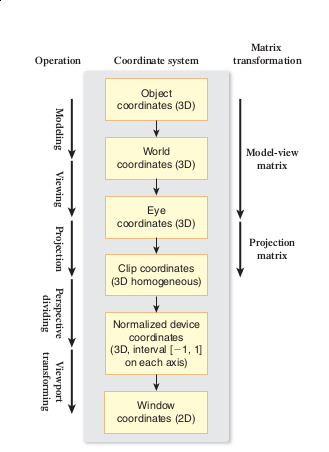
\includegraphics[width =.8\textwidth]{../figuras/viewingpipeline}
    \par\medskip
    Fonte: Adaptado de~\cite{hughes2014computer}.
    \label{viewingpipelinerep}
\end{figure}

\subsection{Coordenadas do Objeto}

O sistema de coordenadas do objeto � considerado o sistema de coordenadas inicial, n�o 
processado de um objeto. Neste sistema as coordenadas s�o locais e o ponto de refer�ncia 
� o centro do objeto. Quando se define uma malha de pol�gonos, os v�rtices est�o nesse 
sistema de coordenadas.

\subsection{Coordenadas do Mundo}
\label{worldcoord}

Nesse est�gio os v�rtices s�o convertidos para um sistema de coordenadas unificado do 
mundo (cena). Essa convers�o � feita multiplicando os v�rtices por uma matriz conhecida 
como matriz de transforma��o. Essa matriz � uma combina��o de transforma��es de 
transla��o, rota��o e escala, podendo ter os tr�s tipos, nenhum deles ou qualquer 
combina��o intermedi�ria (por exemplo apenas transla��o e escala). 

Isso significa que, para uma determinada cena, todos os objetos que possuem uma forma 
associada a estes tamb�m possuem uma matriz de transforma��o associada, essa matriz � 
o recurso utilizado para posicion�-los do mundo da aplica��o.

\subsection{Coordenadas de Visualiza��o}

Nesse est�gio as coordenadas s�o convertidas para o \textit{eye space}, no qual os 
v�rtices s�o posicionados conforme o ponto de vista de uma c�mera virtual, que � um 
objeto abstrato de uma cena o qual possui uma posi��o e uma orienta��o. Nesse est�gio os
objetos da cena s�o posicionados de acordo com esses dois par�metros da c�mera.

A convers�o � feita atrav�s da matriz de visualiza��o, que � constru�da a partir da 
posi��o da c�mera, da sua orienta��o e tamb�m de um vetor que diz qual dos eixos � 
considerado o eixo com a dire��o "para cima"\ da c�mera. Tradicionalmente se utiliza o 
eixo $y$ (i e. $(0,1,0)$), por�m outros eixos podem ser utilizados.

\subsection{Coordenadas Truncadas}

Nesse est�gio ocorre uma normaliza��o do formato do volume de visualiza��o da c�mera. 
Renderizar a cena toda � um processo custoso e redundante pois a c�mera muitas vezes 
n�o � capaz de visualizar a cena toda. Por este motivo, s�o somente renderizados na cena 
os objetos que est�o totalmente ou parcialmente no campo de vis�o de c�mera. Esse campo 
de vis�o � definido por um s�lido com um certo volume e a modelagem desse s�lido � 
dependente da t�cnica de proje��o empregada. 

A proje��o � um processo que converte as coordenadas de um espa�o tridimensional para um 
espa�o truncado. Objetos que est�o parcialmente vis�veis t�m seus v�rtices que est�o fora 
do volume de visualiza��o realocados para as extremidades do mesmo. 
A convers�o � feita atrav�s da matriz de proje��o, e sua constru��o tamb�m � dependente 
da t�cnica de proje��o.

A t�cnica de proje��o utilizada neste trabalho � a proje��o de perspectiva, esta t�cnica 
transforma o volume de visualiza��o em uma pir�mide truncada, conhecida como 
\textit{frustum} de visualiza��o. O topo da pir�mide � chamado de plano perto, e � o 
in�cio da visualiza��o da c�mera. A base da pir�mide � chamada de plano longe, e � o 
fim da visualiza��o da c�mera. Quanto mais pr�ximo os objetos est�o da base da 
pir�mide, menor eles ir�o aparentar na cena.

\subsection{Coordenadas Normalizadas do Dispositivo}

Nesse est�gio � feita uma normaliza��o das coordenadas 3D para um intervalo entre 
$[-1,1]$ para cada um dos eixos. Nessa normaliza��o, $-1$ e $1$ representam os extremos 
do dispositivo tanto na vertical quanto na horizontal.
Esse est�gio n�o � dependente de nenhum argumento da aplica��o e � gerenciado 
pelo componente do hardware respons�vel.

\subsection{Coordenadas da Tela}

As coordenadas chegam nesse est�gio somente na fase final de renderiza��o, que � o 
processo de rasteriza��o (se��o~\ref{renderingpipelinesec}), as coordenadas 3D 
normalizadas s�o convertidas para coordenadas de janela 2D e assim como o est�gio 
anterior, este est�gio � gerenciado pelo hardware. Ap�s esse est�gio, os 
pixels ter�o suas coordenadas definidas para serem devidamente dispostos na tela da 
aplica��o.

\section{Malhas de Pol�gono}

Malhas de pol�gono s�o uma forma de representar objetos em aplica��es gr�ficas, elas s�o 
populares pois requerem um baixo custo computacional. Uma malha consiste em v�rios 
pol�gonos agrupados ao longo de suas arestas para formar a superf�cie do objeto. 

O pol�gono mais utilizado � o tri�ngulo, por alguns motivos que facilitam o seu uso. 
Por exemplo, tr�s v�rtices � o m�nimo necess�rio para se formar um plano, ent�o os 
v�rtices de um tri�ngulo estar�o garantidamente no mesmo plano, o que n�o � verdade 
para outros pol�gonos com maiores dimens�es, e quando todos os pontos de um pol�gono 
n�o s�o coplanares, n�o se sabe como o interior deve ser preenchido nesse caso. 
Tri�ngulos tamb�m s�o pol�gonos at�micos (dividir um tri�ngulo em dois sempre resultar� 
em dois pol�gonos) e qualquer forma pode ser representada como uma subdivis�o de 
tri�ngulos, ou aproximada, caso seja muito complexa~\cite{hughes2014computer}.
Al�m disso, tri�ngulos mant�m sua integridade de forma sobre a maior parte de 
transforma��es afins e proje��es de perspectiva, e a maior parte dos dispositivos de 
hardware comerciais de acelera��o gr�fica s�o otimizados para rasteriza��o de 
tri�ngulos~\cite{gregory2009game}.

\section{Ilumina��o}

Ilumina��o em aplica��es gr�ficas consiste na simula��o do modelo de ilumina��o que h� 
no mundo real. Existem v�rias fontes de luzes diferentes e tamb�m diferentes tipos de 
luz, por exemplo, uma fonte de luz pode ser unidirecional ou multidirecional.

Objetos que est�o mais pr�ximos de uma fonte de luz tendem a ter uma intensidade maior 
das cores presentes em suas superf�cies, e quanto mais se distanciam de uma fonte de 
luz, suas superf�cies tendem a ficar mais escuras. Al�m disso, alguns objetos possuem 
materiais que refletem a luz, como o vidro, e tamb�m que causam a refra��o da luz, os 
modelos de ilumina��o tamb�m s�o capazes de simular estes efeitos. Essa t�cnica de 
simular intensidades de luz diferentes sobre os objetos atrav�s da varia��o dos n�veis 
de escurid�o � conhecida como sombreamento.

Existem seis fen�menos principais que surgem da intera��o entre objetos e ilumina��o, 
que determinam a colora��o modificando ou filtrando a distribui��o de energia da luz 
incidente. Estes fen�menos s�o: reflex�o, transmiss�o, absor��o, difra��o, refra��o e 
interfer�ncia. A maior parte da aten��o na �rea de Computa��o Gr�fica foi dada a modelos 
de reflex�o~\cite{Watt2003GVA}.

H� mais de um modelo de reflex�o dispon�vel na literatura. Por motivos de efici�ncia e 
simplicidade, o modelo utilizado para a aplica��o deste trabalho ser� o modelo de 
sombreamento de Blinn-Phong~\cite{Blinn1977MLR}.

\section{Shaders}

Shaders s�o pequenos programas que s�o executados na GPU, escritos em uma linguagem de 
\textit{shading}, projetada para tornar a programa��o dos shaders f�cil. 
Esses programas s�o utilizados para descrever como processar os dados no 
\textit{pipeline} gr�fico~\cite{hughes2014computer}. Os dados s�o enviados da CPU para 
a GPU atrav�s de uma API gr�fica (ver se��o~\ref{lowlevelrenderer}), onde os shaders 
s�o capazes de referenci�-los e manipul�-los.

Essas linguagens de \textit{shading} lembram vagamente linguagens imperativas 
cl�ssicas, por�m cont�m apenas o necess�rios para o processamento destes dados na GPU. 
Os shaders utilizados com OpenGL por exemplo, s�o escritos em uma linguagem conhecida 
como GLSL, acr�nimo para \textit{OpenGL Shading Language}~\cite{shreiner2013opengl}.

H� v�rias opera��es que os shaders s�o capazes de realizar sobre os dados na GPU, tais 
como: transformar os v�rtices dos objetos de um espa�o para outro (por exemplo, 
do espa�o do objeto para espa�o do mundo), sombreamento, utilizar as coordenadas de 
normais para ilumina��o, \textit{mappings}, utilizar coordenadas de textura para 
aplicar uma certa textura, entre outros.

Existem v�rios tipos diferentes de shader, cada um � respons�vel por uma etapa 
diferente do \textit{pipeline} de renderiza��o. A seguir ser�o listados os diferentes 
tipos de shader, na ordem em que suas fun��es s�o realizadas pelo \textit{pipeline} de 
renderiza��o~\cite{shreiner2013opengl}~\cite{hughes2014computer}:
\begin{itemize}
    \item Vertex Shader: respons�veis pela manipula��o geom�trica dos objetos, realiza 
        transforma��es das posi��es dos v�rtices.
    \item Tessellation Shader: Utiliza descri��es de alto n�vel de superf�cies e produz 
        lista de tri�ngulos a partir delas. Pode receber como \textit{input} os v�rtices 
        e uma estrutura de uma malha, e produzir como \textit{output} uma cole��o de 
        tri�ngulos menores que fornecem uma boa aproxima��o das superf�cies da malha.
    \item Geometry Shader: Podem alterar a lista de tri�ngulos a serem processados nas 
        etapas subsequentes. Um uso popular dos \textit{geometry shaders} � para a 
        renderiza��o por camadas~\cite{shreiner2013opengl}.
    \item Fragment Shader: respons�vel pelo processamento dos fragmentos, que s�o 
        peda�os de pol�gonos que v�o aparecer em um �nico pixel. Colocando de outra 
        maneira, os \textit{fragment shaders} ir�o determinar a cor final de um pixel 
        na tela, por isso neste shader ser�o computadas interpola��es de cores, a 
        ilumina��o aplicada sobre o v�rtice e as texturas, se houver alguma.
    \item Compute Shader: neste shader ser� feito o c�lculo de informa��o arbitr�ria, 
        geralmente utilizado para tarefas que n�o est�o diretamente relacionadas com a 
        renderiza��o de tri�ngulos ou pixels.
\end{itemize}

Um conjunto contendo cada um desses tipos diferentes de shader � conhecido como 
"programa de shader". Primeiramente um programa de shader deve ser criado, depois disso 
todos os shaders s�o individualmente carregados, compilados e adicionados a um 
programa de shader. Ap�s essa etapa de compila��o, o programa ent�o deve ser ligado � 
GPU e est� pronto para ser usado. Uma instru��o para explicitamente utilizar um 
programa de shader � necess�ria antes do processo de renderiza��o ser feito.

Uma aplica��o n�o � restrita a apenas um programa de shader, v�rios programas podem 
ser criados por aplica��o, permitindo o uso alternado destes durante uma execu��o. 
Isso significa que os objetos presentes na cena podem utilizar um programa de shader 
espec�fico para sua renderiza��o e consequentemente seu m�todo de renderiza��o poder� 
ser diferente de outros objetos.

\section{Renderizador Gr�fico de Baixo N�vel}
\label{lowlevelrenderer}

O renderizador gr�fico de baixo n�vel � respons�vel pelos elementos mais t�cnicos da 
renderiza��o. Sua preocupa��o � lidar com as primitivas geom�tricas da maneira o mais 
eficiente poss�vel sem comprometer suas integridades~\cite{gregory2009game}.

Uma de suas fun��es � lidar com a comunica��o entre a aplica��o gr�fica e a GPU, esta 
estar� constantemente recebendo dados da aplica��o durante toda a sua execu��o. Esta 
comunica��o � feita atrav�s de uma API gr�fica, como por exemplo, a API gr�fica 
utilizada para o motor de jogos deste trabalho, o OpenGL~\cite{shreiner2013opengl}, 
que apesar de possuir uma vasta quantidade de comandos diferentes para uma rica 
manipula��o dos recursos da GPU, geralmente h� necessidade de uma grande quantidade de 
c�digo para fazer at� mesmo as rotinas mais simples de uma aplica��o gr�fica. Por isso, 
al�m de utilizar uma API gr�fica, esse componente respons�vel pela renderiza��o de 
baixo n�vel tamb�m geralmente inclui um \textit{wrapper} para os comandos da API, 
condensando v�rias fun��es diferentes em abstra��es de maior n�vel, agilizando o 
desenvolvimento e minimizando a quantidade de erros.

O renderizador de baixo n�vel tamb�m conta com outros componentes, como a ger�ncia da 
matriz de visualiza��o e dos par�metros da proje��o 3D (campo de vis�o, e as posi��es 
dos planos de vis�o). Tamb�m gerencia o estado do hardware gr�fico e dos shaders e
argumentos que controlam as fontes de luz e as texturas~\cite{gregory2009game}.

\section{O \textit{Pipeline} de Renderiza��o}
\label{renderingpipelinesec}

O pipeline de renderiza��o � o componente n�cleo da renderiza��o em tempo real. Ele 
receber� todos os argumentos dos objetos que est�o em cena, das c�meras, dos par�metros 
de proje��o, da ilumina��o, as texturas, equa��es de sombreamento, entre 
outros~\cite{akenine2008real}.

Um pipeline consiste em v�rias etapas que geralmente s�o executadas em sequ�ncia para 
gerar um produto final. No caso do pipeline de renderiza��o, para cada um dos ciclos 
feito o produto final � uma imagem renderizada a partir dos argumentos supracitados, essa 
imagem renderizada � chamada de quadro. Quanto mais eficiente for o pipeline e quanto 
maior o poder computacional do hardware, mais r�pido esses quadros poder�o ser 
renderizados.

Segundo~\cite{akenine2008real}, o pipeline de renderiza��o pode ser dividido em tr�s 
etapas principais: aplica��o, geometria e rasterizador, cada uma destas � um pipeline por 
si s�. A figura~\ref{renderingpipelinerep} apresenta as tr�s etapas principais e suas 
respectivas subdivis�es. A seguir, cada uma destas etapas ser� discutida separadamente.

\begin{figure}[h]
    \centering
    \captionof{figure}{Representa��o do pipeline de renderiza��o com suas tr�s etapas 
    principais, estas tamb�m est�o divididas em suas sub-etapas.}
    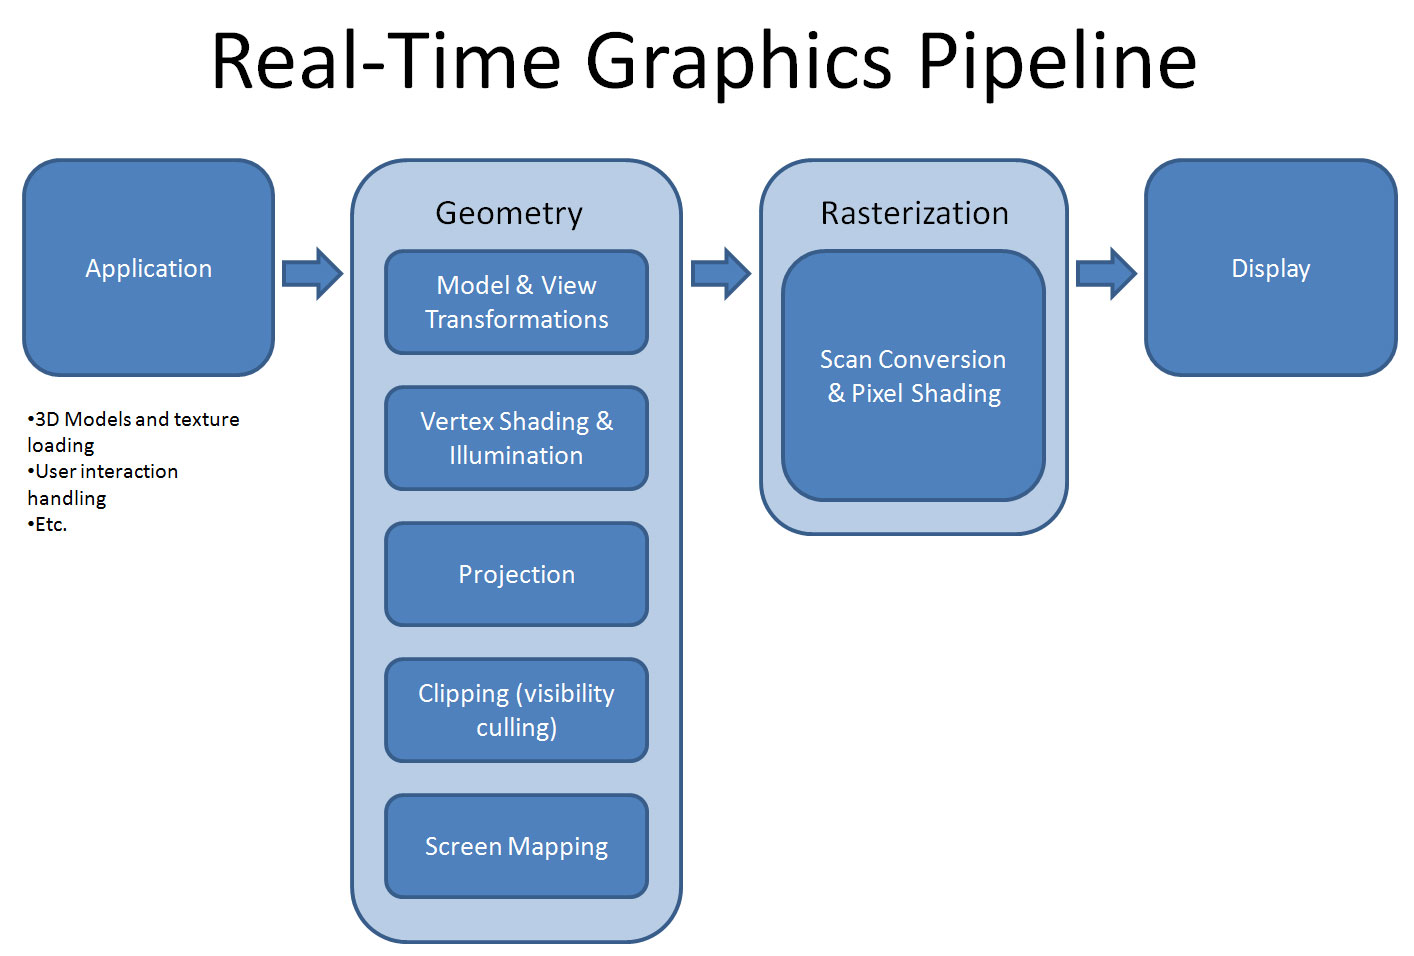
\includegraphics[width =.8\textwidth]{../figuras/renderingpipeline}
    \par\medskip
    Adaptado de: <http://www.cgchannel.com/2010/11/cg-science-for-artists-part-2-the-real-time-rendering-pipeline/>. 
    Acesso em: 27/05/2017.
    \label{renderingpipelinerep}
\end{figure}

\subsection{Aplica��o}

A primeira etapa, a de aplica��o, � executada na CPU\@. Esta � a parte a qual o 
desenvolvedor possui total controle, e na qual a maior parte das otimiza��es podem ser 
feitas para a melhora do desempenho do pipeline. 

Alguns exemplos de computa��es que s�o feitas nesse est�gio s�o: gerenciamento de \textit{inputs}, 
detec��o de colis�o, anima��es de texturas, anima��es atrav�s de transforma��es, ajuste 
de par�metros que s�o utilizados nas outras etapas, etc. Ao final dessa fase, toda a 
geometria e par�metros computados s�o passados � fase de geometria.\ essa passagem de 
dados � considerado o passo mais importante da parte de aplica��o.

\subsection{Geometria}

Na etapa de geometria a maior parte das opera��es sobre v�rtices e pol�gonos s�o feitas. 
Essa etapa ainda � subdividida em outras etapas menores: transforma��o de modelo e de 
visualiza��o, \textit{vertex shading}, proje��o, truncamento e mapeamento para tela. 

A transforma��o de modelo e de visualiza��o converte o sistema de coordenadas de um 
v�rtice para coordenadas do mundo e coordenadas de visualiza��o, respectivamente conforme 
visto na se��o~\ref{viewingpipelinesec}.

O \textit{vertex shading} � o processo pelo qual todos os v�rtices da cena passam e nessa 
parte ser�o definidas suas cores, posi��es, texturas, quantidade de ilumina��o e outros 
atributos. Todos esses atributos s�o ent�o enviados para a etapa de rasteriza��o onde 
ser�o interpolados.

Na etapa de proje��o, ocorre uma transforma��o do volume de visualiza��o, e o seu formato 
depender� do tipo de proje��o utilizada, alterando a percep��o dos objetos da cena. 
Conforme discutido na se��o~\ref{viewingpipelinesec}, a proje��o utilizada neste trabalho 
� a proje��o perspectiva, que transforma o volume de visualiza��o em uma pir�mide 
truncada, chamada de \textit{frustum} de visualiza��o, na qual os objetos mais pr�ximos 
da base da pir�mide aparentam ser menores.

A etapa de truncamento serve para truncar os objetos da cena que est�o sendo parcialmente 
vistos no volume de visualiza��o. Objetos que possuem alguns v�rtices dentro e outros 
fora do volume de visualiza��o precisam ter seus v�rtices que est�o fora realocados para 
os extremos do volume de visualiza��o.

Na �ltima sub-etapa, a de mapeamento para tela, as coordenadas das primitivas truncadas 
dentro do volume de visualiza��o s�o transformadas para a tela. As coordenadas $x$ e 
$y$ de cada primitiva s�o transformadas para formar as coordenadas da tela. As coordenadas 
de tela combinadas com as coordenadas $z$ s�o chamadas de coordenadas de janela. � nessa 
etapa que as coordenadas s�o essencialmente convertidas de tridimensionais para 
bidimensionais.

\subsection{Rasteriza��o}

Com todos os dados para o devido \textit{shading} do objeto, nessa etapa as cores dos 
pixels s�o computadas e definidas, esse � o processo conhecido como rasteriza��o, que � 
a convers�o dos v�rtices em coordenadas de janela juntamente com a informa��o de 
\textit{shading} para pixels desenhados na tela.
Assim como a etapa de geometria, a etapa de rasteriza��o tamb�m � dividida em sub-etapas, 
que s�o: configura��o dos tri�ngulos, \textit{triangle traversal}, \textit{pixel shading} 
e combina��o.

Na etapa de configura��o dos tri�ngulos, os dados sobre as superf�cies dos tri�ngulos 
s�o computados. Esses dados s�o utilizados para a interpola��o de v�rias informa��es 
de \textit{shading} produzida na etapa de geometria. Etapa feita por opera��es fixas 
do hardware dedicado para essa parte.

Na etapa de \textit{triangle traversal} s�o procurados os pixels que est�o dentro de 
um tri�ngulo, ou seja, que pertencem ao plano formado pelos tr�s v�rtices de um dos 
tri�ngulos presentes na tela. Para cada um dos pixels encontrados � gerado um 
fragmento. As propriedades dos fragmentos de cada tri�ngulo s�o geradas utilizando 
dados interpolados entre os tr�s v�rtices.

No \textit{pixel shading}, s�o feitas todas as computa��es de \textit{shading} pixel 
por pixel, usando os dados interpolados como \textit{input}, resultando em uma ou mais cores 
para serem passadas � pr�xima etapa. Esta etapa, ao contr�rio das outras que s�o 
feitas por fun��es fixas do hardware dedicado, � feita por n�cleos program�veis da 
GPU, nomeadamente pelo \textit{fragment shader}. Esse shader ser� respons�vel por 
aplicar texturas, ilumina��o, entre outros em cada um dos fragmentos.

Por fim, na combina��o a informa��o de cada pixel � armazenada em um \textit{buffer} 
de cores, que cont�m cada um dos componentes RGB da cor final. A unidade da GPU 
respons�vel por essa etapa n�o � completamente program�vel, por�m altamente 
customiz�vel.
A cor resultante da etapa anterior (\textit{pixel shading}) � combinada com a cor 
atualmente armazenada no \textit{buffer}.

Essa etapa tamb�m � respons�vel por resolver a visibilidade, ou seja, armazenar no 
\textit{buffer} de cores somente as cores das primitivas que est�o vis�veis a partir 
do ponto de vista da c�mera. Para a maior parte dos hardwares gr�ficos, isso � feito com 
o algoritmo do \textit{Z-buffer}. Esse algoritmo foi originalmente proposto por Edwin 
Catmull~\cite{Catmull1974}, seu funcionamento consiste no uso de um \textit{buffer} de 
profundidade, disposto em uma matriz bidimensional que armazena a profundidade de cada 
um dos pixels da tela. Quando um objeto precisa ser renderizado em um pixel j� 
utilizado, o m�todo compara as duas profundidades e caso o novo objeto esteja mais 
pr�ximo do observador, o pixel � ent�o sobrescrito por este objeto e o novo valor de 
profundidade substitui o antigo no \textit{buffer}.

Todos os \textit{buffers} combinados formam o chamado \textit{frame buffer}, que em 
consequ�ncia cont�m toda a informa��o de um quadro de uma cena renderizada. A tela exibe 
os conte�dos do \textit{buffer} de cores.

\section{O \textit{Loop} de Jogo}
\label{gameloopsec}

O \textit{loop} do jogo � onde os componentes funcionam em conjunto para proporcionar o que 
define um jogo: uma aplica��o interativa em tempo real. 
Sistemas interativos em tempo real podem ser divididos em tr�s m�dulos principais: 
recebimento de \textit{inputs}, processamento e apresenta��o dos 
resultados~\cite{dalmau2004core}.

Jogos possuem restri��es de tempo para realizar todas as 
suas rotinas, se o sistema n�o for capaz de fazer seu trabalho dentro do limite de 
tempo ir� falhar. Uma vez que sistemas em tempo real s�o supostos fazer suas tarefas 
em tempo real, se um jogo n�o for capaz de fazer isso, o usu�rio (nesse caso o 
jogador) n�o receber� um \textit{feedback} cont�nuo, e o jogo n�o fornecer� a 
interatividade que deveria. Um \textit{loop} de jogo pode ser implementado com a 
finalidade de satisfazer essas restri��es~\cite{Joselli2010}.

Nos jogos eletr�nicos, o sistema de \textit{inputs} corresponde ao gerenciamento do dispositivo 
de \textit{inputs}, como mouse, teclado ou controlador de jogo; o processamento � respons�vel 
por tomar as decis�es que afetam o estado do jogo, e a apresenta��o � respons�vel por 
mostrar os resultados desses dois outros est�gios, atrav�s de �udio e 
v�deo~\cite{valente2005real}. 

Elaborar um \textit{loop} de jogo significa organizar esses tr�s m�dulos, e seus subm�dulos na 
certa para deixar a simula��o o mais fiel o poss�vel da experi�ncia desejada. 
Considerando os m�dulos citados, o \textit{loop} do jogo pode ser dividido da seguinte 
maneira:
\begin{itemize}
    \item Detec��o e gerenciamento de \textit{inputs}
    \item Est�gio de processamento
    \item Est�gio de apresenta��o
\end{itemize}

O est�gio de processamento � ainda subdividido em outras partes, onde cada uma 
corresponde a um aspecto diferente do estado do jogo, como detec��o de colis�es, 
simula��es f�sicas, a IA do jogo, aplica��es das regras do jogo, etc. Estas portanto, 
tamb�m devem ser organizadas na ordem correta. No est�gio de apresenta��o s�o 
reproduzidos todos os �udios necess�rios e a cena � renderizada na tela com os 
resultados dos est�gios anteriores.

Uma medida de desempenho de aplica��es gr�ficas que tamb�m � utilizada para medir a 
frequ�ncia com a qual esses \textit{loops} s�o executados � a quantidade de quadros por 
segundo (\textit{Frames per Second}) que s�o renderizados na tela, conhecido como 
FPS. Cada quadro que aparece na tela representa uma imagem constru�da e apresentada 
pela aplica��o.

O desempenho de um jogo, al�m de ser dependente das otimiza��es feitas a n�vel de 
software, � tamb�m dependente da configura��o de hardware da plataforma na qual ser� 
executado. Portanto, um mesmo jogo pode rodar com um FPS diferente dependendo da 
plataforma utilizada, visto que a atualiza��o do estado do jogo � dependente da 
quantidade de quadros constru�dos, uma mesma sequ�ncia de eventos pode ter um 
resultado diferente dependendo do poder computacional do hardware. 

Para evitar esse problema, � necess�rio tornar o est�gio de processamento independente 
da taxa de FPS. Isso pode ser feito adicionando um par�metro de tempo ao est�gio de 
processamento. Esse par�metro corresponde ao tempo decorrido entre a atualiza��o 
atual e a �ltima atualiza��o do processamento feita~\cite{valente2005real}, e � 
conhecido como \textit{delta time}, indicando uma diferen�a de tempo.

Al�m da separa��o do est�gio de processamento em sub-tarefas, � importante salientar 
que nem todas possuem a mesma necessidade de atualiza��o que outras. Por exemplo, a IA 
n�o precisa ser atualizada com a mesma frequ�ncia que a simula��o f�sica, 
� necess�rio somente quando um agente precisa tomar uma decis�o. A renderiza��o por 
outro lado, proporcionar� um resultado melhor quanto mais atualizada esta for, desde 
que n�o comprometa o desempenho geral do sistema. Por isso, uma forma de otimizar o 
desempenho � atualizar cada um dos componentes somente quando necess�rio.

\section{Interpola��es}

Na se��o~\ref{gameloopsec}, foi discutido o problema da atualiza��o do estado do jogo em 
rela��o � taxa de quadros por segundo com a qual a aplica��o est� sendo executada, e 
como esse problema podia ser solucionado adicionando um par�metro que indicasse o tempo 
decorrido entre o �ltimo quadro e o atual.

Interpola��o � um dos recursos utilizados na solu��o deste problema, e � utilizada para 
qualquer caso em que se queira passar uma no��o de locomo��o ou movimento entre os 
diversos quadros, seja atrav�s de anima��es, aplica��o de for�as, rota��es, etc.

Caso se queira adicionar um vetor de velocidade a um objeto, esse objeto passar� a ter 
duas velocidades: a velocidade inicial, a qual ele j� possui, e a velocidade alvo, a qual 
� uma combina��o de sua velocidade inicial com a nova velocidade aplicada. Se a altera��o 
da velocidade inicial para a velocidade alvo fosse feita de um quadro para o outro, o 
objeto teria uma acelera��o instant�nea (ou desacelera��o) completamente n�o natural e 
n�o realista. A interpola��o serve para calcular os pontos intermedi�rios entre esses 
dois extremos a partir de um par�metro que determinar� quantos pontos intermedi�rios 
ser�o gerados. No exemplo da velocidade, esse par�metro pode ser uma combina��o entre 
uma acelera��o e o tempo decorrido entre um quadro e outro (\textit{delta time}). Dessa 
maneira, a altera��o da velocidade ser� feita de uma maneira gradual e independente da 
taxa de quadros por segundo.

A classe geral de fun��es utilizadas para interpola��es s�o chamadas de curvas 
param�tricas. Dado os dois pontos sendo interpolados, uma interpola��o entre estes 
pode ser entendida como uma curva formada entre suas posi��es, onde o par�metro 
supracitado determinar� em que posi��o se est� nessa curva. O exemplo mais simples de uma 
curva param�trica � dado por:

\begin{equation}
    \begin{aligned}
        L(t) = 1 - t \cdotp P_0 + t \cdotp P_1
    \end{aligned}
\end{equation}

\vspace{1cm}

Esta � uma interpola��o linear, onde $L(t)$ � um ponto intermedi�rio, $P_0$ � o ponto 
inicial, $P_1$ � o ponto alvo e $t$ � o par�metro utilizado para controlar a posi��o em 
que se est� na linha relativa a $P_0$ e $P_1$. Nota-se que $t$ varia em um intervalo 
entre $[0,1]$, quanto mais pr�ximo de $0$, mais pr�ximo de $P_0\ $ se estar� e quanto 
mais pr�ximo de $1$ mais pr�ximo de $P_1\ $ se estar�. 

Esse conceito de interpola��o linear pode ser estendida para vetores e quaternions por 
exemplo, permitindo a aplica��o gradual de for�as e de rota��es.
Na �rea de Computa��o Gr�fica, � popular a utiliza��o do jarg�o "lerp"\ para se referir 
� interpola��o linear, uma abrevia��o de \textit{Linear Interpolation}.

\subsection{Interpola��o Entre Vetores}

A interpola��o linear entre dois vetores � semelhante � interpola��o entre dois pontos 
vista anteriormente. A diferen�a � que o c�lculo da interpola��o � feito componente a 
componente, semelhante �s outras opera��es entre dois vetores:

\begin{equation}
    \begin{aligned}
        Lerp(u,v,t) = (1 - t \cdotp u_x + t \cdotp v_x, \\
                      1 - t \cdotp u_y + t \cdotp v_y, \\
                      1 - t \cdotp u_z + t \cdotp v_z)
    \end{aligned}
\end{equation}

\vspace{1cm}

\subsection{Interpola��o Entre Quaternions}

Para interpolar dois quaternions, � necess�rio calcular o menor caminho do �ngulo formado 
entre os dois, visto$\ $ que a interpola��o � feita de maneira circular. Para realizar este 
c�lculo, utiliza-se o produto escalar entre os dois quaternions, que retornar� o cosseno 
do �ngulo e dependendo do seu valor, par�metros diferentes s�o utilizados:

\begin{equation}
    \begin{aligned}
        \cos \theta = q_1 \cdotp q_2 \\
        t_1 = 1 - t \\
        q_i = 
        \begin{cases}
            (q_1 \cdotp t_1) + (q_2 \cdotp t) & \quad \text{se } \cos \theta > 0 \\
            (q_1 \cdotp t_1) + (q_2 \cdotp -t) & \quad \text{se } \cos \theta < 0 \\
        \end{cases}
    \end{aligned}
\end{equation}

\vspace{1cm}

Onde $q_1$ e $q_2$ s�o os dois quaternions sendo interpolados, $t$ � o par�metro de 
interpola��o e $q_i$ � o quaternion resultante da interpola��o. � importante ressaltar 
que $q_i$ deve ser normalizado ao final da interpola��o.

Quaternions ainda possuem um outro tipo de interpola��o, a interpola��o linear esf�rica, 
que � um pouco mais custosa de se calcular do que a interpola��o linear normal, por�m 
possui uma precis�o maior. Essa interpola��o � conhecida como "slerp", abrevia��o de 
\textit{Spherical Linear Interpolation}. Utilizando os mesmos par�metros da outra 
interpola��o, a slerp � dada por:

\begin{equation}
    \begin{aligned}
        \theta = \arccos(q_1 \cdotp q_2) \\
        t_1 = \sin((1 - t) \cdotp \theta / \sin \theta) \\
        t_2 = \sin(t \cdotp \theta / \sin \theta) \\
        q_i = (t_1 \cdotp q_1) + (t_2 \cdotp q_2)
    \end{aligned}
\end{equation}

\vspace{1cm}

Assim como na interpola��o linear normal, aqui $q_i$ tamb�m deve ser normalizado ao final 
da opera��o.

\section{Considera��es Finais do Cap�tulo}

Neste cap�tulo foram apresentados os fundamentos utilizados para o desenvolvimento do 
trabalho proposto, que possui um alto fator interdisciplinar.
A modelagem orientada a dados � um termo que surgiu recentemente, por�m seu conceito de 
uso eficiente e sequencial da mem�ria j� � utilizado a mais tempo. Foram apresentados 
alguns de seus principais princ�pios, suas diferen�as com a programa��o orientada a 
objetos, que atualmente � considerada o padr�o na ind�stria, e como a restrutura��o de 
c�digo utilizando essa abordagem pode proporcionar uma melhora no desempenho de uma 
aplica��o.

Os motores de jogos revolucionaram o modo como os jogos s�o feitos na ind�stria atrav�s 
da clara separa��o entre o conte�do t�cnico e o criativo de um jogo. Foi explicado o 
surgimento deste conceito, a filosofia de implementa��o de um motor de jogo, a 
import�ncia da integra��o apropriada de seus componentes e tamb�m foram apresentados 
alguns exemplos de componentes comuns em motores de jogos.
Foram apresentados diversos conceitos matem�ticos que s�o amplamente utilizados na 
�rea de computa��o gr�fica, e tamb�m as diferentes estruturas comumente utilizadas e 
suas respectivas funcionalidades e m�todos.

Foram apresentados os \textit{pipelines} de visualiza��o e renderiza��o, dois 
conceitos importantes em aplica��es gr�ficas que consistem em etapas que processam os 
dados desde o seu carregamento no sistema at� serem transformados em pixels na tela, 
e como o renderizador gr�fico de baixo n�vel auxilia nas etapas da renderiza��o.
Outros conceitos importantes de Computa��o Gr�fica tamb�m foram explicados, como 
\textit{shaders}, ilumina��o e malhas de pol�gono.

Todos os componentes s�o combinados para a forma��o de um \textit{loop} principal, que ser� 
encarregado de receber e gerenciar os \textit{inputs} do jogador, atualizar os 
componentes que necessitam faz�-lo, e apresentar os resultados computados. Esse \textit{loop} 
� conhecido como \textit{loop} de jogo, neste cap�tulo esse conceito foi introduzido e detalhado.
Tamb�m foi discutido sobre alguns de seus problemas, como a necessidade de diferentes 
frequ�ncias de atualiza��o de cada um dos componentes, e tamb�m como os resultados 
das atualiza��es podem ser diferentes dependendo do poder computacional do hardware 
utilizado. Foi apresentada uma solu��o para este problema, e tamb�m uma medida de 
desempenho popular para jogos, a taxa de quadros por segundo (FPS).

Por fim, foi apresentado o conceito de interpola��es e como o seu uso se relaciona com 
o problema da varia��o de FPS em jogos. Al�m disso, foram apresentados exemplos de 
implementa��o da interpola��o linear para vetores e quaternions.

\chapter{Trabalhos Relacionados}
\label{relatedworkscap}

Neste cap�tulo ser�o apresentados alguns trabalhos encontrados na literatura que est�o relacionados 
com a proposta deste trabalho. A maioria dos trabalhos apresentados concentra-se em criar 
funcionalidades �nicas para um motor de jogos e tamb�m nas melhores pr�ticas para o 
desenvolvimento de motores de jogos, por�m nenhum destes trabalhos explora o uso da 
modelagem orientada a dados.
Apesar de nenhum deles estar diretamente relacionado com a proposta deste trabalho, os 
autores tamb�m tinham como um dos objetivos desenvolver um motor de jogos eficiente e 
bem estruturado.

\citeonline{deFreitas2012GEC} prop�s um modelo de motor de jogos com uma 
arquitetura baseada em componentes, na qual as entidades do jogo s�o definidas atrav�s 
da agrega��o de componentes, em contraste com os modelos cl�ssicos os quais utilizam 
hierarquia de classes e heran�as m�ltiplas, que leva a problemas como forte 
interdepend�ncia das entidades, conflito de nomenclaturas e heran�as repetidas.

Esta arquitetura baseada em componentes atualmente � utilizada em motores de jogos 
comerciais populares, como � o caso do motor de jogos de prop�sito geral 
Unity3D\footnote{Site do Unity3D: https://unity3d.com}. Nesse 
modelo, uma entidade pode ter caracter�sticas diferentes adicionadas a ela atrav�s da 
adi��o de componentes configur�veis, como um componente renderizador de imagens, um 
reprodutor de �udios, um corpo suscet�vel � aplica��o de for�as f�sicas, entre outros. 
Este modelo de arquitetura permite ent�o a cria��o de entidades com uma maior 
flexibilidade, adaptabilidade e independ�ncia, al�m de n�o apresentar os problemas do 
uso de heran�a.

O trabalho deles prossegue ent�o, para explicar seus diferenciais, como a utiliza��o de 
entidades que permitem a sua reconfigura��o din�mica em diferentes 
momentos da aplica��o. Consequentemente isso permite flexibilidade e extensibilidade 
at� mesmo em tempo de execu��o. Por fim eles apresentam as decis�es de design que os 
permitiram atingir esses objetivos.

\citeonline{Anderson2008} discute em seu trabalho alguns problemas ainda pendentes 
em se tratando de desenvolvimento de motores de jogos, e incentiva a pesquisa no campo 
de arquitetura e design de motores de jogos. 

Primeiramente, os autores comentam sobre o aumento significativo do uso motores de 
jogos, pelo aumento da produtividade que estes proporcionam. Depois � mencionada a falta 
de literatura e pesquisa a respeito de modelagem e arquitetura de motores de jogos em 
geral, sendo que a maioria do material encontrado tem �nfase apenas na implementa��o dos 
componentes individuais, enquanto que as estrat�gias utilizadas para a modelagem dos 
motores como um todo n�o s�o comentadas, sendo ent�o dif�cil encontrar material que 
apresente uma explica��o minuciosa sobre a modelagem e estrutura��o da arquitetura de 
um motor de jogos.

Depois dessa introdu��o, s�o mencionados alguns problemas persistentes nessa �rea, que 
podem ser potenciais �reas de pesquisa a respeito de motores de jogos. Primeiramente,
s�o: h� uma falta de conven��o sobre as terminologias utilizadas em desenvolvimento de 
jogos, frequentemente levando a problemas de comunica��o e pesquisa eficiente e confus�o 
entre os estudantes novos na �rea. 

O segundo problema mencionado � a dificuldade na determina��o do limite entre o que faz 
parte do jogo propriamente dito e o que faz parte do motor de jogos. N�o h� uma 
defini��o concreta sobre o que � um motor de jogos e existem v�rias vers�es diferentes, 
frequentemente levando ao equ�voco no entendimento sobre o conceito de um motor de 
jogos. 

O terceiro problema mencionado � sobre as decis�es de modelagem do motor de jogos, e 
como diferentes g�neros de jogos afetam essas decis�es, pois algumas estrat�gias em 
espec�fico beneficiam somente uma certa classe de jogos. � levantada ent�o a 
quest�o da possibilidade de defini��o de um motor de jogos que � eficiente para qualquer 
jogo independente do seu tipo.

O quarto problema mencionado � sobre o impacto que as rotinas de baixo-n�vel dos motores 
de jogos causam na modelagem de alto-n�vel do mesmo, comentando sobre a constante 
evolu��o da tecnologia utilizada em dispositivos de hardware ou nas interfaces do 
software e suas capacidades, e como essas mudan�as podem afetar a evolu��o de um ou 
m�ltiplos componentes do motor de jogos.

O �ltimo problema mencionado � sobre as melhores conven��es e pr�ticas de programa��o 
que devem ser utilizadas na modelagem de um motor de jogos. Como os motores de jogos 
est�o em constante crescimento e evolu��o desde seus desenvolvimentos iniciais, a 
adi��o de novas funcionalidades pode ser problem�tica ou at� mesmo imposs�vel, se os 
objetivos no motor de jogos n�o foram bem definidos no in�cio do projeto, ou se sua 
arquitetura n�o foi bem estruturada. Os autores ponderam ent�o se existe um conjunto de 
melhores pr�ticas para evitar ou reduzir estes problemas.

\citeonline{Keenan2011} salientam a import�ncia da defini��o de uma boa arquitetura para 
o desenvolvimento de um motor de jogos. Em seu trabalho, ele menciona os problemas 
relacionados com a m� estrutura��o do motor de jogos, e como a cria��o de um sistema 
flex�vel e modularizado pode evitar esses problemas, al�m de proporcionar outras 
vantagens.
Como o seu trabalho � para fins educativos, o restante do artigo trata sobre a 
cria��o de um curso sobre arquitetura de jogos, no qual o foco n�o � a implementa��o dos 
componentes separados do motor de jogos, mas sim a utiliza��o das melhores pr�ticas de 
programa��o e modelagem para a constru��o de um motor de jogos com uma arquitetura 
robusta.

\citeonline{Zhu2016ECG} prop�em uma nova metodologia para o desenvolvimento de jogos, 
chamada de \textit{Engine- Cooperative Game Modeling} (ECGM), um modelo h�brido 
que combina duas outras metodologias: \textit{Model-Driven Game Development} (MDGD) e a 
cadeia de ferramentas do motor de jogos, com �nfase nos aspectos t�cnicos. A motiva��o 
de seu trabalho � que nenhuma das abordagens para o MDGD na literatura demonstrou 
convincentemente uma boa integra��o do MDGD com a cadeia de ferramentas do motor de 
jogos.
No restante do trabalho, � descrito o funcionamento desta metodologia proposta, e como 
ela pode fornecer uma melhoria na modelagem dos projetos ao utilizar o MDGD levando em 
considera��o a cadeia de ferramentas tipicamente utilizadas em motores de jogos.

Um trabalho mais relacionado ao tema modelagem orientada a dados � o proposto 
por~\citeonline{Fontana2017}, no qual a MOD � utilizada no desenvolvimento de uma 
ferramenta \textit{opensource} de projeto f�sico de circuitos integrados. No trabalho 
s�o discutidos os principais conceitos da MOD, como esta pode ser utiliada para aprimorar 
a qualidade do \textit{software} e como pode ser utilizada no contexta de porblemas de 
projeto f�sico, que assim como jogos, tamb�m precisa lidar com uma substancial quantidade 
de dados.

Para validar os fundamentos discutidos, foi desenvolvido um sistema utilizando um padr�o de 
projeto conhecido como modelo entidade-componente, que consiste em decompor um problema 
em um conjunto de entidades e seus componentes (chamados de propriedades). Os resultados 
obtidos foram comparados com um outro sistema com uma abordagem orientada a objetos para 
testar o desempenho do sistema com MOD.\@ As m�tricas escolhidas foram o tempo de execu��o e 
a quantidade de \textit{cache misses} para dois problemas diferentes. 

Os resultados obtidos pelos autores mostram que um problema em um cen�rio com boa 
localidade de data, isto �, cen�rios que requerem poucas propriedades de cada entidade, a 
MOD � cerca de 90\% mais r�pida que a orienta��o a dados. Enquanto que em um cen�rio com 
uma m� localidade de data, que requer o acesso a uma quantidade superior de propriedades 
diferentes das diferentes entidades do sistema, a MOD apresenta um desempenho apenas 6\% 
pior em m�dia.

\section{Considera��es Finais do Cap�tulo}

Dados os problemas mencionados nos trabalhos relacionados, percebe-se que a maior 
dificuldade no desenvolvimento de um motor de jogos n�o consiste na implementa��o dos 
componentes individuais que comp�em o motor, mas sim na integra��o adequada destes 
componentes e no projeto e modelagem eficientes do motor. 

Como foi mencionado, a maior parte do material encontrado concentra-se na implementa��o 
dos componentes individuais e nas otimiza��es feitas sobre estes, como por exemplo as 
otimiza��es que podem ser feitas em algoritmos de intelig�ncia artificial comumente 
utilizados em jogos. Como a proposta deste trabalho se concentra exatamente em uma 
abordagem diferente para a modelagem e estrutura��o dos componentes do motor de jogos 
e consequentemente na integra��o destes, foi poss�vel encontrar trabalhos apenas 
parcialmente relacionados.

Al�m disso nenhum dos trabalhos encontrados deu �nfase nos problemas que podem surgir 
do uso da programa��o orientada a objetos em jogos, e quais s�o as alternativas ou 
pr�ticas que podem contornar esses problemas. Apesar de alguns trabalhos mencionarem 
maneiras de melhorar a arquitetura e projeto de um motor de jogos, ou proporcionar 
uma maior flexibilidade e extensibilidade, nenhum deles discute sobre como melhorar a 
estrutura desses componentes, principalmente levando em considera��o a evolu��o do 
hardware, conforme mencionado por Anderson~\cite{Anderson2008}.

Devido ao fato da modelagem orientada a dados ainda n�o ser um conceito muito difundido, 
n�o foi poss�vel encontrar trabalhos que tivessem �nfase especificamente neste t�pico.

\chapter{Otimiza��es para motores de jogos atrav�s de modelagem 
orientada a dados}
\label{proposalcap}

Para testar as otimiza��es proporcionadas pela modelagem orientada 
a dados, um motor de jogos foi desenvolvido em duas vers�es 
diferentes: uma utilizando os conceitos da programa��o orientada a 
objetos, e outra utilizando modelagem orientada a dados,
visando � otimiza��o da comunica��o entre o processador e a mem�ria.
A vers�o com abordagem de programa��o orientada a objetos ser� 
referida como primeira vers�o, ou vers�o OO (orientada a objetos). A 
outra vers�o com a abordagem de modelagem orientada a dados ser� referida 
como segunda vers�o, ou vers�o OD (orientada a dados).
Al�m de utilizar os conceitos da MOD, tamb�m � necess�rio 
utilizar conceitos de Computa��o Gr�fica, �lgebra Linear e Geometria Anal�tica, Teoria 
de Grafos, Processamento de Imagens, F�sica, entre outros.

Conforme explicado na se��o~\ref{secgameengine}, um motor de jogos � uma combina��o de 
diversos componentes diferentes que juntos comp�em a parte l�gica de um jogo digital. As 
se��es seguintes discutir�o sobre os componentes implementados que foram julgados 
necess�rios para o desenvolvimento do motor de jogos que � o objeto de estudo deste 
trabalho, bem como as diferen�as entre as implementa��es.

Al�m dos componentes, tamb�m ser�o explicadas as estrat�gias empregadas para a 
implementa��o de outros elementos importantes discutidos previamente no 
cap�tulo~\ref{theorycap} que fazem parte da estrutura de um motor de jogos, como o 
\textit{pipeline} de renderiza��o e o loop de jogo.

Como um motor de jogos por si s� n�o � suficiente para se gerar an�lises e resultados, 
pois seu objetivo � dar suporte ao desenvolvimento de uma outra aplica��o, al�m do 
desenvolvimento do motor, foi necess�rio o desenvolvimento de uma aplica��o 
que utilize as funcionalidades do motor para realmente 
verificar sua efici�ncia. A aplica��o desenvolvida � id�ntica para 
as duas vers�es do motor.

A an�lise de desempenho das principais fun��es da aplica��o 
permitir� a compara��o entre as duas abordagens e a efici�ncia da 
MOD. Al�m das altera��es necess�rias nos componentes do motor, h� 
tamb�m altera��es a serem feitas na aplica��o de teste 
desenvolvida, estas ser�o apresentadas para demonstrar a convers�o 
entre as abordagens. Apesar das diferen�as, nem todos os componentes 
sofreram altera��es entre as duas vers�es, por este motivo n�o 
ser�o apresentadas altera��es para todos os componentes descritos 
nesse cap�tulo.

\begin{figure}[h]
    \centering
    \captionof{figure}{UML simplificado contendo os principais componentes do motor.}
    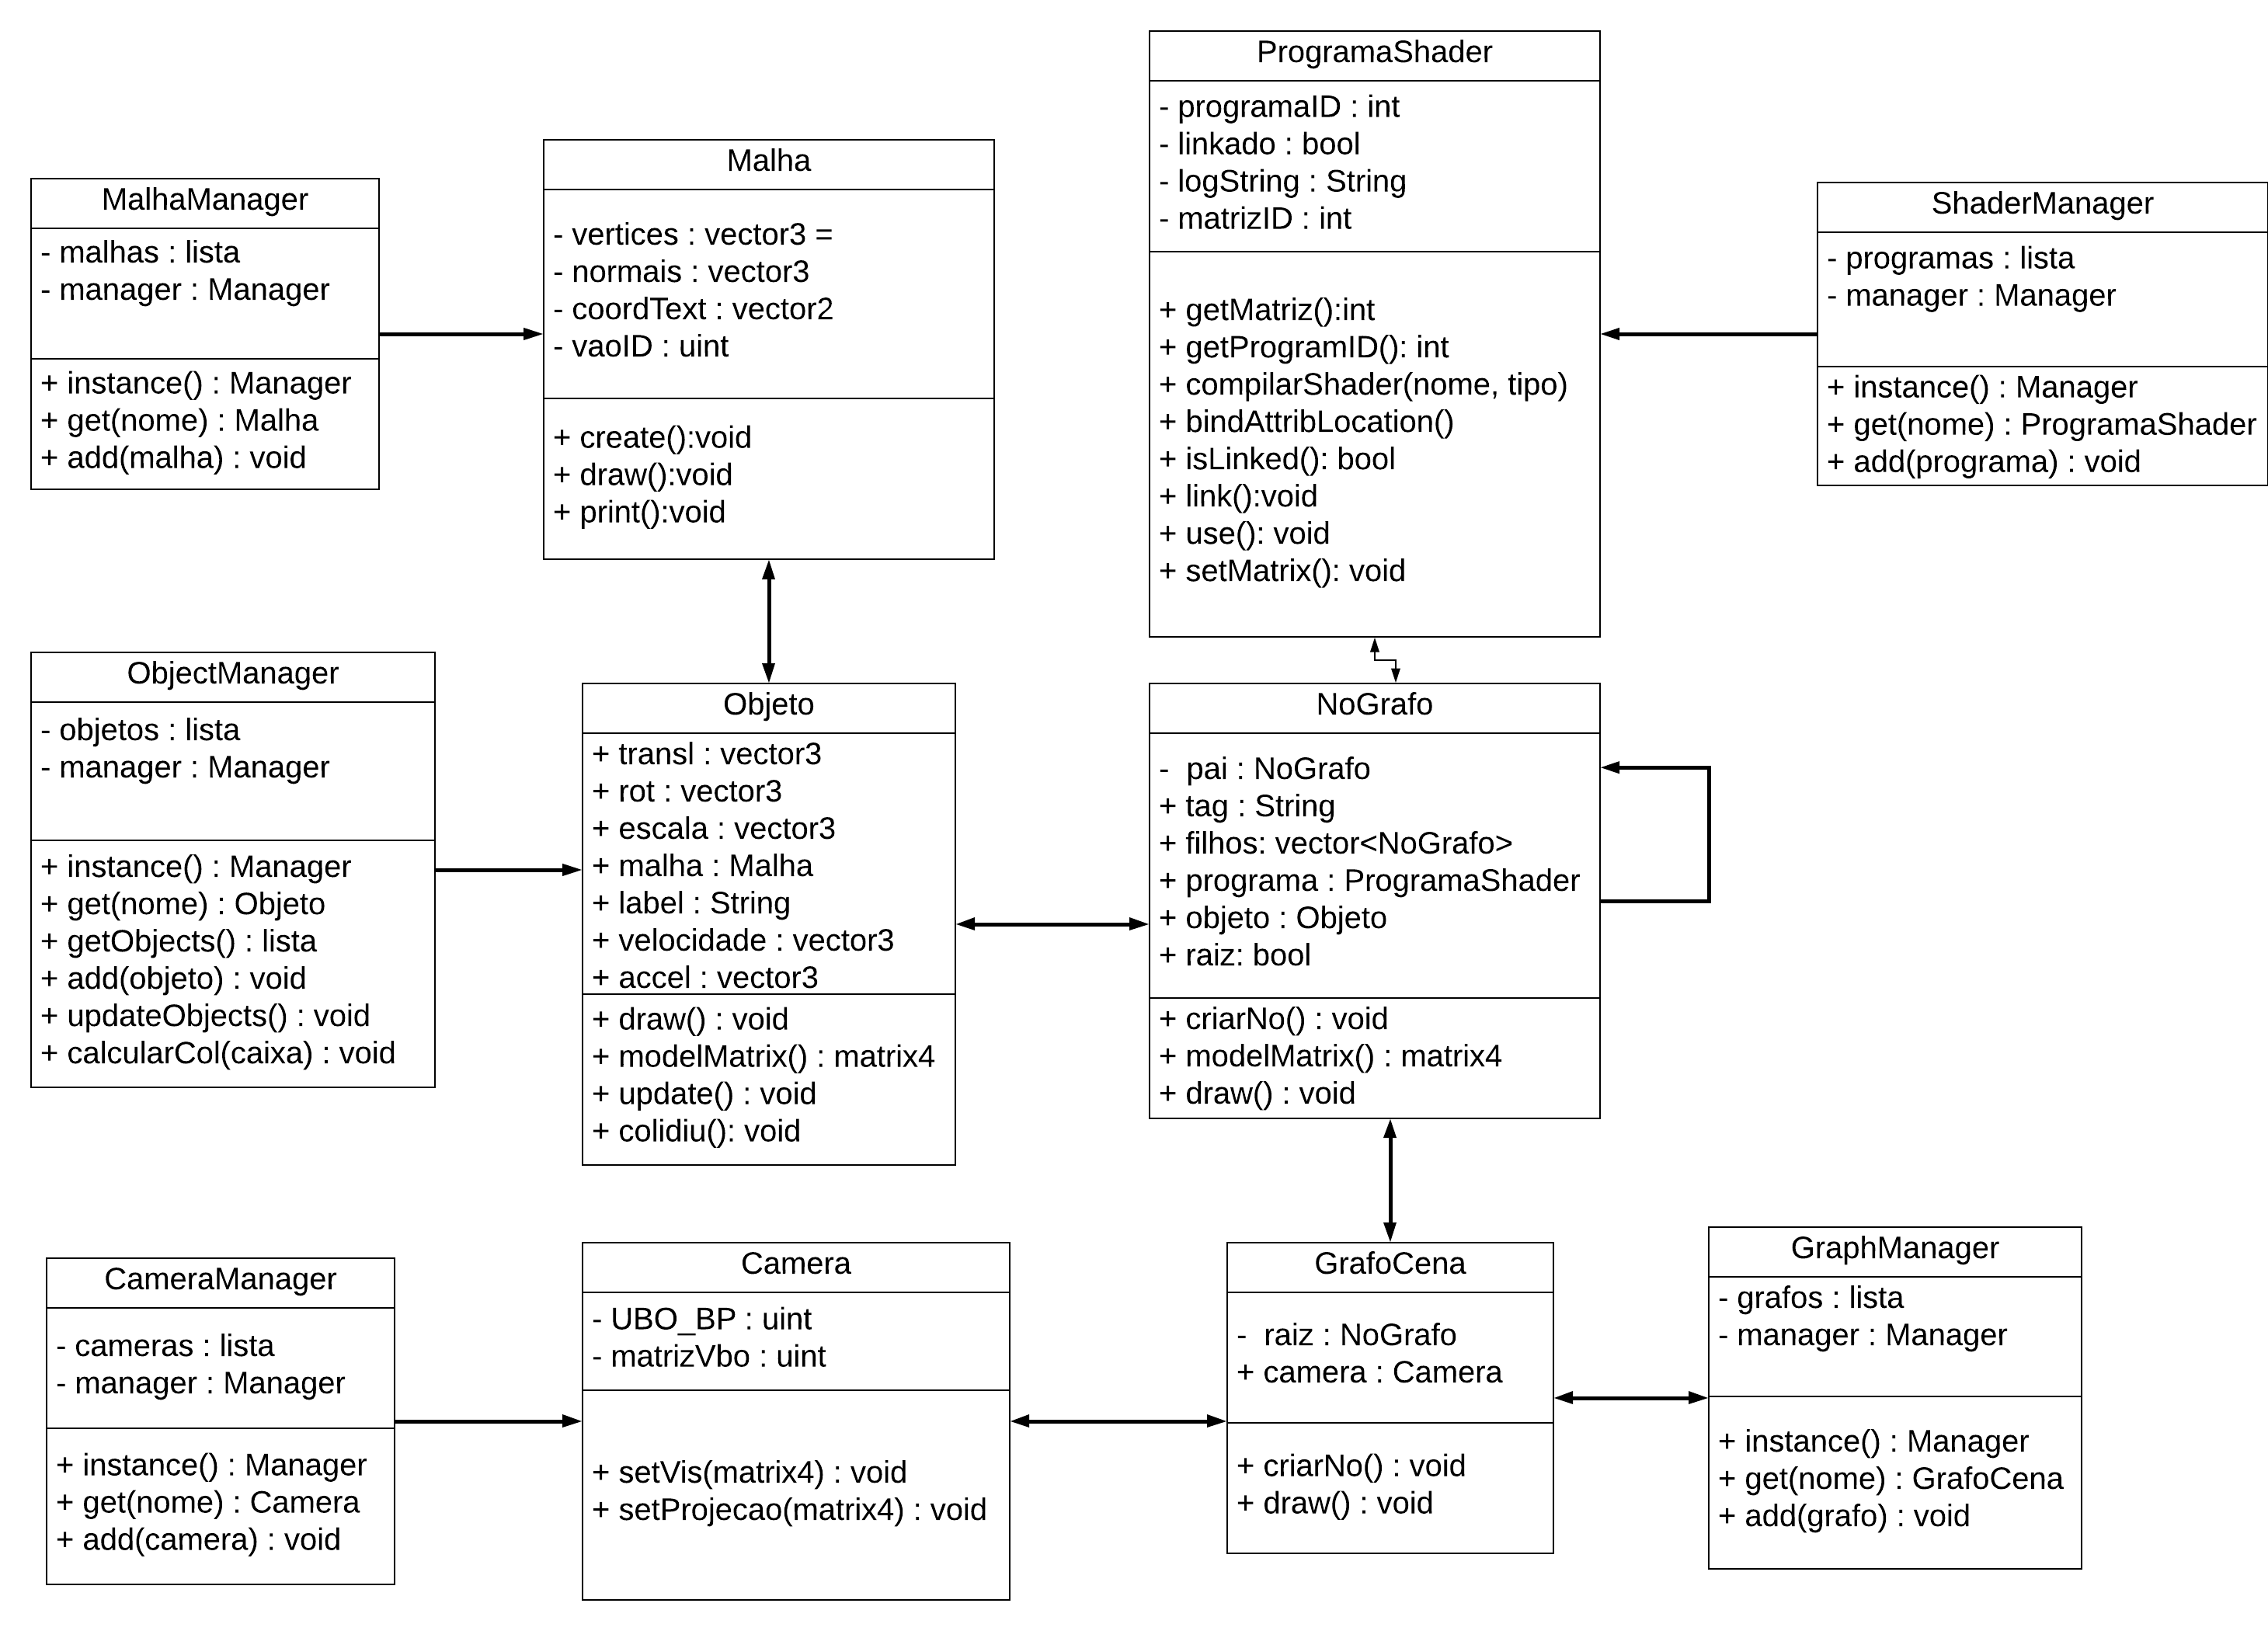
\includegraphics[width =.8\textwidth]{../figuras/uml_engine}
    \par\medskip
    Fonte: autoria pr�pria
    \label{umlengine}
\end{figure}

A figura~\ref{umlengine} cont�m um diagrama de classes com as principais
classes do motor e as rela��es entre estas na vers�o orientada a objetos. Os 
componentes do motor juntos cont�m o m�nimo necess�rio para executar uma 
aplica��o gr�fica 3D utilizando openGL. O componente gr�fico � composto pelas 
classes ProgramaShader, GrafoCena, NoGrafo, Camera e Malha. O componente da 
f�sica � composto pela classe Objeto. 

Para o gerenciador de recursos foi 
utilizado o padr�o de \textit{singletons} de design de software, no qual as 
classes que s�o \textit{singletons} restringem a instancia��o de objetos da 
classe para exatamente um. As classes do tipo Manager apresentadas na 
figura~\ref{umlengine} s�o \textit{singletons} que controlam o armazenamento e 
acesso aos principais recursos da aplica��o, que s�o as malhas, objetos, grafos 
de cena, cameras e shaders.

O primeiro passo feito para realizar a convers�o do motor para uma abordagem 
orientada a dados, conforme descrito na sess�o~\ref{secdataorienteddesign}, 
foi analisar o fluxo de dados necess�rio para que cada um dos componentes 
funcionem apropriadamente, e especificar quais s�o os dados gerados 
por cada componente. Depois de determinar o fluxo, o pr�ximo passo foi 
descrever as transforma��es de dados que cada componente precisa 
realizar.

Ap�s analisar os componentes do motor e a aplica��o desenvolvida, 
pode-se observar que o fluxo de dados ocorre na seguinte ordem:\\
\begin{enumerate}
    \item Os recursos externos s�o carregados no sistema (\textit{shaders} e malhas).
    \item Os objetos e o grafo de cena s�o criados e alocados.
    \item Inicia-se o ciclo principal do programa:
        \begin{enumerate}
           \item Atualiza��o dos objetos.
           \item Verifica��o de colis�es.
           \item A c�mera atualiza a matriz de visualiza��o e proje��o.
           \item O grafo de cena � renderizado.
        \end{enumerate}
\end{enumerate}

Com o fluxo de dados definido, � necess�rio analisar as 
transforma��es necess�rias dos dados. A parte relevante do 
sistema a ser analisada � o ciclo principal, pois � a �nica parte 
do fluxo de dados que ser� executada em tempo real.

A primeira etapa do ciclo principal � a atualiza��o dos objetos. 
Primeiramente a acelera��o do objeto � atualizada atrav�s de 
f�rmulas arbitr�rias, posteriormente a velocidade � atualizada 
utilizando a acelera��o. Com a velocidade atualizada a �ltima 
parte � atualizar a transla��o e a rota��o, ambas s�o atualizadas 
atrav�s da velocidade.

A segunda etapa � a verifica��o de colis�es, isso � feito 
utilizando as dimens�es de uma caixa retangular e o componente 
de transla��o do objeto. O procedimento de verifica��o de colis�o 
simplesmente testa se o componente de transla��o do objeto n�o 
ultrapassa as bordas da caixa.

A terceira etapa consiste na atualiza��o das matrizes de 
visualiza��o e proje��o da cena. A atualiza��o ocorre somente uma 
vez por frame, e como h� somente uma c�mera na cena, essa etapa 
n�o possui muito potencial para otimiza��o.

A �ltima etapa � a renderiza��o do grafo de cena. Para cada n� 
presente no grafo, essa etapa � 
dividida em tr�s partes: c�lculo das coordenadas do objeto, 
convers�o dessas coordenadas para coordenadas do mundo, e a 
renderiza��o do grafo.

O c�lculo das coordenadas do objeto � feito 
atrav�s da multiplica��o entre a transla��o, rota��o e escala do 
objeto atribu�do ao n�. A convers�o das 
coordenadas do objeto para as coordenadas do mundo � feita utilizando 
as coordenadas do objeto e a hierarquia do grafo de cena. Por fim 
a �ltima parte � a renderiza��o propriamente dita, na qual n�o 
h� processamento de dados, somente chamadas de m�todos da API do 
openGL sobre dados j� processados. Os dados necess�rios para a 
renderiza��o de um n� s�o a malha atribu�da ao objeto deste n�, 
o programa de shader atribu�do ao n� e as coordenadas convertidas.

Com o fluxo de dados definido, assim como as transforma��es sobre 
os dados necess�rias, � poss�vel determinar quais s�o os dados 
m�nimos necess�rios para a execu��o de aplica��o e como 
agrup�-los.

Seguindo a premissa da MOD de descrever as transforma��es de 
dados sempre para o caso mais prov�vel, as estruturas de dados 
utilizadas para o motor na vers�o orientada a dados foram 
feitas considerando que em uma aplica��o sempre haver� 
v�rias inst�ncias de \textit{shaders}, malhas, objetos 
e n�s do grafo de cena.

\begin{figure}[h]
    \centering
    \captionof{figure}{Estruturas utilizadas na ver�o orientada a dados do motor.}
    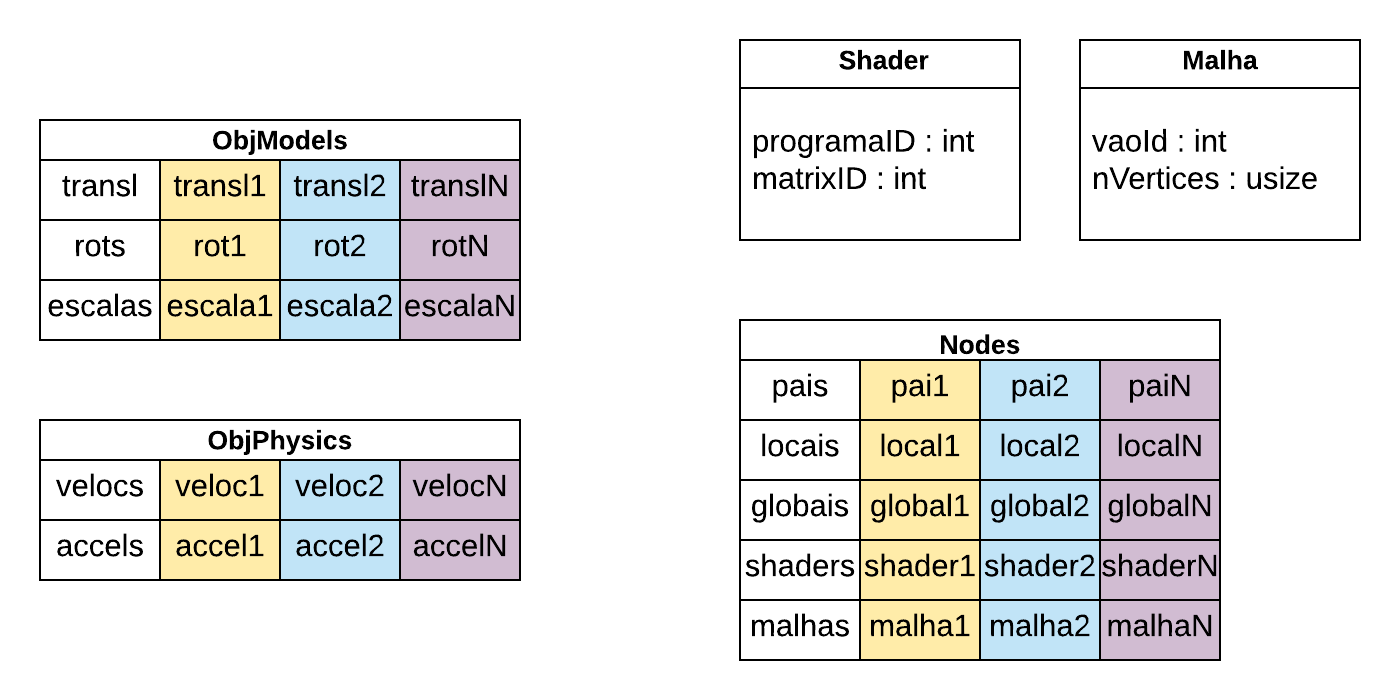
\includegraphics[width =.8\textwidth]{../figuras/dodengine}
    \par\medskip
    Fonte: autoria pr�pria
    \label{dodengine}
\end{figure}

A figura~\ref{dodengine} apresenta as estruturas utilizadas no ciclo principal de 
execu��o da aplica��o com uma abordagem orientada a dados, utilizando o layout SoA 
discutido na se��o~\ref{secdataorienteddesign}. As classes de programa de 
shader e malha foram separadas em duas partes: interfaces para a cria��o de shaders 
e malhas a partir de arquivos externos, e estruturas simples contendo somente dados 
primitivos utilizados no ciclo principal. As estruturas de n�s e objetos possuem 
\textit{containers} de $N$ elementos para os atributos principais das respectivas 
classes da vers�o orientada a objetos. A classe de objeto foi dividida em duas 
estruturas: uma para os dados da matriz de transforma��o (transla��o, rota��o e 
escala), e a outra para dados de f�sica (velocidade e acelera��o).

Cada entidade no sistema possui seu identificador �nico representado 
por um n�mero inteiro positivo e seus atributos s�o espalhados pelas estruturas 
que cont�m \textit{containers}. Ou seja, a refer�ncia ao item $0$ 
de qualquer um dos \textit{containers} apresentados na 
figura~\ref{dodengine} refere-se � mesma entidade. Atrav�s desse 
ID �nico de uma entidade os componentes s�o capazes de transformar 
e mover os dados entre si.

A seguir ser�o descritos com detalhes os componentes um a um 
presentes nos motores implementados. Para os componentes que 
possuem diferen�as de implementa��o entre as duas vers�es tamb�m 
ser�o discutidas quais foram as mudan�as necess�rias para o 
desenvolvimento da vers�o orientada a dados.

\section{Biblioteca Matem�tica}

Utilizando os conceitos discutidos na se��o~\ref{secmathconcepts}, foi 
desenvolvido uma biblioteca matem�tica o mais minimalista o poss�vel, contendo somente 
as estruturas e fun��es necess�rias para se realizar os testes e obter os resultados 
desejados deste trabalho. 

A biblioteca � uma das partes do motor mais extensivamente utilizada pois uma 
consider�vel parcela dos componentes necessitam de sua utiliza��o. Al�m disso, todas as 
malhas e outros dados que s�o enviados aos \textit{shaders} program�veis s�o armazenados em 
estruturas dessa biblioteca, como as matrizes de transforma��o, visualiza��o e proje��o, 
fontes de luz, texturas, etc.

A biblioteca possui tr�s estruturas: vetores, matrizes e quaternions. Para cada uma das 
estruturas h� diversas fun��es diferentes associadas a elas. Al�m das fun��es associadas 
�s estruturas, existem tamb�m fun��es e utilidades que n�o s�o inerentes a nenhuma delas, 
somente da biblioteca em si. 

Para todas as estruturas, o tipo das vari�veis utilizadas s�o os n�meros reais, mais 
especificamente, ponto flutuante de precis�o simples. A precis�o simples � a utilizada em 
jogos ou outras aplica��es gr�ficas pois geralmente esse n�vel de precis�o j� � o 
suficiente, al�m de ter os benef�cios de consumir menos mem�ria e realizar opera��es 
aritm�ticas com mais efici�ncia do que pontos flutuantes de precis�o 
dupla~\cite{Verth:2008}.

\subsection{Vetores}

Para os vetores, h� uma estrutura separada para os vetores 3D e para os 4D. Os vetores 
2D n�o estar�o presentes na biblioteca pois n�o ter�o uso para a aplica��o pretendida.

Al�m do acesso individual a cada um dos componentes do vetor e sua manipula��o direta, 
as seguintes fun��es s�o suportadas para vetores:
\begin{itemize}
    \item Opera��es aritm�ticas: adi��o e subtra��o entre vetores, multiplica��o ou 
        divis�o por escalar e igualdade entre vetores.
    \item C�lculo da magnitude de um vetor.
    \item Magnitude ao quadrado: essa fun��o � similar � magnitude, com a diferen�a de 
        que essa fun��o n�o calcula a raiz quadrada da soma dos quadrados dos 
        componentes. Caso a finalidade do c�lculo da magnitude seja apenas para comparar 
        dois vetores, esse fun��o j� basta, e � mais eficiente pois poupa o c�lculo 
        custoso da raiz quadrada.
    \item Normaliza��o: existe duas fun��es diferentes, uma delas apenas normaliza o 
        vetor, enquanto a outra mant�m o vetor inalterado e retorna a sua vers�o 
        normalizada.
    \item Produto escalar entre dois vetores.
    \item Produto vetorial entre dois vetores. Essa fun��o � exclusiva para vetores 
        3D.
    \item Interpola��o linear entre dois vetores.
\end{itemize}

\subsection{Matrizes}

Assim como os vetores, as matrizes tamb�m possuem uma estrutura separada para matrizes 
$3 \times 3$ e $4 \times 4$, por�m somente esses dois tipos de matrizes quadradas est�o 
presentes pois s�o as �nicas necess�rias para a implementa��o da aplica��o.

As matrizes possuem suporte � acesso individual a cada elemento e tamb�m a manipula��o 
direta destes. Al�m disso, possuem as seguintes funcionalidades:
\begin{itemize}
    \item Adi��o, subtra��o e igualdade entre matrizes.
    \item Multiplica��o por escalar.
    \item C�lculo da matriz transposta.
    \item Multiplica��o entre matrizes.
    \item Multiplica��o entre uma matriz e um vetor. Essa fun��o trata o vetor como uma 
        matriz linha ou matriz coluna, dependendo da ordem. Essa fun��o requer uma 
        implementa��o diferente para cada uma das duas possibilidades de ordem dos 
        operandos.
    \item C�lculo da matriz inversa e do determinante da matriz. Essas duas fun��es s�o 
        exclusivas para matrizes $3 \times 3$.
\end{itemize}

\subsection{Quaternions}

S� h� uma estrutura para os quaternions, com acesso aos seus componentes escalar $t$, e 
ao vetorial $x,y,z$. Um quaternion pode ser constru�do tanto passando o valor dos seus 
quatro componentes, quanto passando um �ngulo e um eixo, �til para se fazer uma 
transforma��o de rota��o.

A estrutura de quaternion possui as seguintes funcionalidades associadas:
\begin{itemize}
    \item Adi��o, subtra��o e igualdade entre quaternions.
    \item Multiplica��o por escalar.
    \item Multiplica��o entre quaternions.
    \item Produto escalar entre quaternions.
    \item Extra��o do �ngulo do quaternion.
    \item Extra��o do eixo do quaternion.
    \item C�lculo da norma.
    \item Normaliza��o. Semelhante aos vetores, pode simplesmente normalizar ou retornar 
        uma c�pia normalizada.
    \item Convers�o para matriz.
    \item Interpola��o linear e interpola��o linear esf�rica entre quaternions.
\end{itemize}

\subsection{Outras Utilidades}

Al�m das fun��es mencionadas anteriormente, ainda existem algumas outras fun��es que 
servem como conven��es para facilitar o processo de desenvolvimento e minimiza��o de 
c�digo escrito.

A biblioteca matem�tica tamb�m possui fun��es que n�o est�o associadas com nenhuma 
estrutura, por exemplo, fun��es trigonom�tricas tais como: cotangente, convers�o de 
graus para radianos e vice-versa.

H� constantes que tamb�m s�o utilizadas com frequ�ncia, como PI, epsilon, e um limitante 
arbitr�rio de pontos flutuantes. Esse limitante � utilizado para calcular a igualdade 
entre pontos flutuantes e consequentemente, todas as estruturas implementadas. Essa 
igualdade deve ser calculada de maneira diferente da igualdade entre inteiros, isso 
porque ao longo da execu��o, os pontos flutuantes acumulam "lixo", pequenos erros de 
c�lculo em suas menores casas decimais, por esse motivo, dois n�meros reais podem ser 
iguais, mas a opera��o de igualdade retorna falso por causa desses erros acumulados. A 
igualdade entre dois pontos flutuantes pode ser calculada da seguinte maneira: 

\begin{equation}
    \begin{aligned}
        d = |x - y| \\
        x = y \iff d < T \\
        x,\ y,\ d,\ T \in \mathbb{R}
    \end{aligned}
\end{equation}

\vspace{.5cm}

Onde $x$ e $y$ s�o os operandos, $d$ � a diferen�a entre eles e $T$ � o limitante de 
pontos flutuantes.

Por exemplo, considerando dois n�meros de ponto flutuante: $x = 2.0$ e $y = 2.000001$, a 
determina��o do limitante $T$ ir� tamb�m determinar se esses dois n�meros s�o iguais ou
n�o. Para um $T = 10^{-5}$, teria-se:

\begin{equation}
    \begin{aligned}
        d = |x - y| = 0.000001 = 10^{-6}\\
        x = y \iff 10^{-6} < 10^{-5} \\
        x,\ y,\ d,\ T \in \mathbb{R}
    \end{aligned}
\end{equation}

\vspace{.5cm}

Neste caso, para a escolha de $T = 10^{-5}$, os n�meros $x$ e $y$ s�o iguais.

Construir matrizes manualmente � um processo demorado e prop�cio a erros, por isso, a 
biblioteca matem�tica possui diversas fun��es que criam matrizes prontas que s�o 
frequentemente utilizadas. A seguir ser�o listadas matrizes que podem ser criadas a 
partir de fun��es espec�ficas:
\begin{itemize}
    \item Matriz identidade $3 \times 3$ ou $4 \times 4$.
    \item Matriz nula $3 \times 3$ ou $4 \times 4$.
    \item Convers�o de uma matriz $3 \times 3$ para uma $4 \times 4$ e vice-versa.
    \item Matriz de transla��o, criada a partir de um vetor 3D contendo o deslocamento em 
        cada um dos eixos.
    \item Matriz de rota��o, criada a partir de um �ngulo e do eixo de rota��o. Existe 
        uma fun��o com esses mesmos par�metros para criar um quaternion ao inv�s de uma 
        matriz.
    \item Matriz de escala, criada a partir de um vetor 3D contendo o fator de escala 
        para cada um dos eixos.
    \item Matriz de visualiza��o, criada a partir de um vetor indicando a posi��o, um 
        vetor indicando a dire��o e um vetor que representa o eixo que aponta para cima.
    \item Matriz de proje��o perspectiva, criada a partir de um �ngulo que representa o 
        campo de vis�o, a propor��o da tela (largura por altura), a dist�ncia at� o 
        plano perto e a dist�ncia at� o plano longe.
\end{itemize}

\section{Componente Gr�fico}

O componente gr�fico de um motor de jogos � um dos principais m�dulos, devido a 
consider�vel quantidade de sub-tarefas que ele realiza, alguns exemplos s�o: definir 
as malhas de cada objeto, gerenciamento da c�mera, gerenciamento das cenas, 
manipula��o da parte configur�vel do \textit{pipeline} de renderiza��o, configura��o 
das otimiza��es de renderiza��o, interfaceamento com a API gr�fica atrav�s da 
utiliza��o do renderizador gr�fico de baixo-n�vel (se��o~\ref{lowlevelrenderer}) e 
tamb�m de outras maneiras, como por exemplo a utiliza��o de fun��es que comp�em uma 
interface para a manipula��o das vari�veis contidas nos \textit{shaders}, defini��o da 
ordem de renderiza��o dos objetos da cena, entre outros. 

A parte gr�fica � a �ltima a ser atualizada em um quadro, antes da renderiza��o da 
cena. As atualiza��es dessa parte visual consistem em altera��es nas propriedades dos 
objetos que est�o na cena, como suas matrizes de transforma��o, cores, texturas, 
programa de \textit{shader} que ir�o utilizar, suas malhas e seus efeitos de 
pr�-processamento ou p�s-processamento. Al�m disso, h� atualiza��es de outros 
par�metros n�o relacionados aos objetos geom�tricos, como a matriz de visualiza��o e 
proje��o, par�metros das fontes de ilumina��o, altera��o da resolu��o da tela, entre 
outros.

Para o motor desenvolvido neste trabalho, h� apenas a implementa��o do 
\textit{vertex shader} e do \textit{fragment shader}, pois estes s�o os �nicos que s�o 
indispens�veis para a constru��o do \textit{pipeline} de renderiza��o, o restante dos 
\textit{shaders} possuem implementa��es padr�es j� fornecidas pelo 
OpenGL~\cite{shreiner2013opengl}.

Da parte manipul�vel do \textit{pipeline} de renderiza��o, o motor permite a 
altera��o direta das posi��es dos objetos na cena, a hierarquia dos objetos, suas 
malhas e seus programas de \textit{shader}. Al�m disso, � tamb�m poss�vel a altera��o 
dos par�metros das matrizes de visualiza��o e proje��o e tamb�m os par�metros de 
ilumina��o atrav�s de vari�veis uniforme.

As vari�veis uniformes s�o utilizadas para qualquer par�metro existente nos 
\textit{shaders} que se deseja modificar ao longo da execu��o da aplica��o. Suas 
diferen�as em rela��o �s vari�veis normais � que as vari�veis uniformes s�o 
modificadas apenas no n�vel de aplica��o, sendo usadas nos \textit{shaders} apenas 
para a leitura de seus valores. Outra diferen�a � que a declara��o de uma vari�vel 
uniforme � global no contexto do programa de \textit{shader}, e 
n�o somente no \textit{shader} que a vari�vel uniforme foi 
declarada~\cite{wolff2013opengl}.

\subsection{C�mera}

A c�mera estabelece o modo como a cena � visualizada pelo espectador. � basicamente 
constitu�da de dois componentes, a matriz de visualiza��o, que ir� determinar de qual 
posi��o a cena ser� vista e a partir dessa posi��o, de qual �ngulo a cena ser� vista. 
H� tamb�m a matriz de proje��o, que ir� aplicar uma das t�cnicas de proje��o sobre a 
cena e ir� tamb�m remover da renderiza��o os objetos que est�o fora do campo de vis�o 
da c�mera. 

Uma c�mera pode ser configurada de maneiras diferentes, e os par�metros depender�o de 
como � pretendida a intera��o do espectador com a cena. Alguns exemplos de 
comportamento incluem:
\begin{itemize}
    \item C�mera livre: possui livre movimenta��o ao longo dos tr�s eixos
    \item C�mera 2.5D: possui livre movimenta��o ao longo de dois eixos, e o terceiro 
        � fixado, geralmente � o eixo que aponta para cima.
    \item C�mera esf�rica: a c�mera se move em torno de uma esfera que geralmente 
        engloba a cena inteira, por�m o tamanho desta esfera pode ser alterado, 
        causando os efeitos de \textit{zoom in} e \textit{zoom out}.
\end{itemize}

Pode existir mais de uma c�mera na mesma cena e suas vis�es podem aparecer 
simultaneamente na tela, geralmente � feito um esquema de divis�o de tela para que isso 
seja poss�vel.

Por ser uma classe consideravelmente simples, n�o h� diferen�a na classe de c�mera 
entre as vers�es do motor. Conforme visto na figura~\ref{dodengine}, uma c�mera 
armazena dois inteiros positivos, um para armazenar o �ndice do bloco de vari�veis 
uniformes, e outro para armazenar o \textit{vertex array object} da c�mera, que � 
um �ndice para a posi��o da mem�ria da GPU na qual os dados das matrizes est�o 
armazenados. A classe de c�mera possui apenas dois m�todos: um para alterar a matriz 
de visualiza��o, e outro para alterar a matriz de proje��o.

\subsection{Grafo de Cena}
\label{scenegraphsection}

Consiste em uma estrutura para definir a hierarquia dos objetos de uma cena e as 
propriedades de cada um. Essa estrutura � um grafo ac�clico direcionado cujos n�s 
formam uma hierarquia. Cada 
n� possui um conjunto de propriedades, tais propriedades podem ser herdadas de seu 
n� pai e podem ser passadas para os n�s filhos. Por exemplo, se um n� possui uma 
matriz de transforma��o, ent�o nas coordenadas do mundo seus filhos n�o ter�o mais o 
centro do mundo como refer�ncia, mas sim o centro representado pela matriz de 
transforma��o do seu pai, e suas posi��es finais ser�o dadas pela combina��o da suas 
matrizes de transforma��o com a do seu pai.

O esquema dos n�s no grafo de cena permite f�cil reutiliza��o de componentes, se dois 
objetos id�nticos forem necess�rios na cena, basta criar um n� com as propriedades e 
utilizar instancia��o, e tamb�m permite flexibilidade, cada n� pode ter sua pr�pria 
malha, programa de \textit{shader}, entre outros atributos~\cite{hughes2014computer}. 
As liga��es permitem uma f�cil constru��o de hierarquia, e tamb�m torna trivial coisas 
como uma mudan�a de posi��o de um subgrupo inteiro de objetos.

\begin{figure}[h!]
    \centering
    \captionof{figure}{Exemplo de um grafo de cena descrevendo parcialmente um objeto 
    que representa um carro.}
    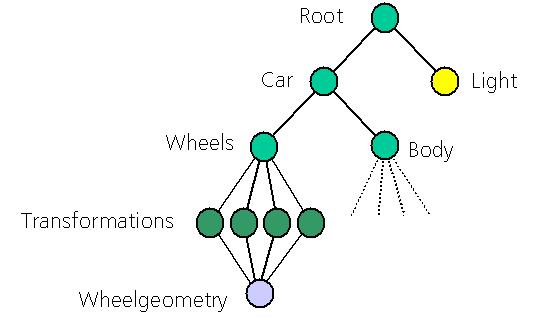
\includegraphics[width =.6\textwidth]{../figuras/scenegraph}
    \par\medskip
    Adaptado de: <http://www.opensg.org/htdocs/doc-1.8/PageScenegraph.html>. Acesso 
    em: 05/06/2017.
    \label{scenegraphexample}
\end{figure}

A figura~\ref{scenegraphexample} demonstra um exemplo de um grafo de cena que est� 
representando parcialmente um carro utilizando hierarquia, nele h� um n� que 
representa uma roda, este n� possui quatro inst�ncias e estas compartilham uma mesma 
malha que descreve a geometria da roda. Os n�s da roda s�o filhos do n� que representa 
o carro como um todo.

O grafo de cena � utilizado para gerenciar o posicionamento dos objetos da aplica��o e 
tamb�m para controlar a renderiza��o destes atrav�s da chamada do m�todo \textit{draw}. 
Na vers�o orientada a objetos do motor, o grafo de cena � divido em duas classes diferentes, uma 
para armazenar a raiz do grafo e a c�mera utilizada, e outra para armazenar os dados de 
um n� do grafo, esta segunda classe possui a maioria das propriedades e funcionalidades 
do grafo de cena. Al�m do m�todo \textit{draw}, um n� pode criar um n� filho, 
armazenando-o em um vetor de filhos. Outras propriedades do n� incluem: um programa de 
\textit{shader}, um objeto, um ponteiro para o n� pai e uma \textit{string} de 
identifica��o.

Na abordagem orientada a dados, as duas classes que representam o grafo de cena foram 
reduzidas a somente uma estrutura, que cont�m \textit{arrays} cont�guos das mesmas 
propriedades da vers�o orientada a objetos, conforme discutido na 
se��o~\ref{proposalcap}, essa estrutura segue o \textit{layout} de armazenamento de 
dados SoA. A raiz do grafo 
sempre ser� o primeiro elemento em todos os \textit{arrays}, a c�mera foi desacoplada 
do grafo e seu armazenamento foi movido para outra parte. O vetor de filhos foi 
removido e a hierarquia � definida somente pela refer�ncia ao n� pai de cada n�.

\begin{lstlisting}[frame=single, caption={M�todo draw vers�o OO}, label=oodraw]
1  void draw() {
2      if (object == nullptr) {
3          throw RenderException("N� sem objeto");
4      }
5      if (shaderProgram == nullptr) {
6          shaderProgram = getProgramFromParent();
7          if (shaderProgram == nullptr) {
8              throw RenderException("N� sem shader");
9          }
10     }
11     Matrix4 modelMatrix = this->getModelMatrix();
12     shaderProgram->use();
13     shaderProgram->setUniform("Matrix", modelMatrix);
14     object->drawObject();
15     if (!children.empty()){
16         int i;
17         for (i = 0; i < (int)children.size(); i++) {
18             children[i]->draw();
19         }
20     }
21 }
\end{lstlisting}

O m�todo \textit{draw} � o principal do grafo de cena, por ser 
utilizado no loop principal da aplica��o para controlar a 
renderiza��o do grafo. O c�digo~\ref{oodraw} apresenta a 
implementa��o do m�todo \textit{draw} na vers�o OO do motor.

As linhas 2 e 5 cont�m instru��es com condicionais verificando o 
estado do n�, a primeira para verificar se o n� est� sem objeto, 
e a segunda para verificar sem o n� est� sem shader. Na linha 11 
� chamado um m�todo recursivo para se obter a matriz de 
transforma��o do n� a partir do n� pai, sendo que a matriz de 
transforma��o do n� raiz � a matriz identidade.

Nas linhas 12 e 13 s�o chamados dois m�todos do programa de shader, 
o primeiro para especificar ao \textit{openGL} que aquele programa de shader 
ser� utilizado. O segundo m�todo altera o valor da vari�vel 
uniforme "Matrix" contida no programa para o valor da matriz 
de transforma��o calculado para o n�.

Na linha 14 � chamado o m�todo \textit{drawObject} do objeto, 
que � um \textit{wrapper} para a fun��o de renderizar tri�ngulos 
do \textit{openGL}, a qual necessita dos dados da malha vinculada 
ao objeto. A linha 15 cont�m uma condicional para verificar o 
estado do vetor de filhos, e se o n� possuir pelo menos um filho, 
� iniciado o processo recursivo de renderiza��o dos filhos.

\begin{lstlisting}[frame=single, caption={M�todo draw vers�o OD}, label=oddraw]
01  void calcularLocais(transl, rots, escalas, out_locais) {
02      for (i = 1; i < nObjetos; i++) {
03      out_locais[i] =  math::translate(transl[i]) *
04                          rots[i].toMatrix() *
05                          math::scale(escalas[i]);
06      }
07  }
08  void calcularGlobais(locais, pais, out_globais) {
09      for (i = 1; i < nObjetos; i++) {
10      out_globais[i] = out_globais[pais[i]] * locais[i];
11      }
12  }
13  void renderizarNos(globais, shaders, malhas) {
14      for (i = 1; i < nObjetos; i++) {
15      glUseProgram(shaders[i].programID);
16      glUniformMatrix4fv(shaders[i].matrixID, ..., globais[i]);
17      glBindVertexArray(malhas[i].vaoId);
18      glDrawArrays(GL_TRIANGLES, 0, meshes[i].nVertices);
19      }
20  }
21
22  void draw() {
23      calcularLocais(...);
24      calcularGlobais(...);
25      renderizarNos(...);
26  }
\end{lstlisting}

O c�digo~\ref{oddraw} apresenta o m�todo \textit{draw} para a 
vers�o OD do motor, alterado de acordo com as mudan�as feitas nas 
estruturas do motor. Para evitar que muitas propriedades das 
entidades sejam utilizadas em uma transforma��o, o m�todo foi 
dividido em tr�s partes diferentes: c�lculo das coordenadas locais 
(coordenadas do objeto), c�lculo das coordenadas globais (coordenadas 
do mundo), e a renderiza��o propriamente dita. Nota-se que todas 
as subfun��es consistem em loops que percorrem as propriedades de 
todas as entidades, al�m disso, o elemento 0 de todas as 
propriedades nunca � processado por ser reservado para a raiz.

O c�lculo das coordenadas locais (linhas 01 a 07) � feito 
multiplicando-se a transla��o, rota��o e escala de cada objeto e 
armazenando os valores resultantes no vetor de sa�da 
\textit{out\_locais}. O c�lculo das coordenadas globais (linhas 08 a 
12) � feito com as coordenadas locais calculadas na etapa anterior 
e o vetor de pais, respons�vel por manter a hierarquia do grafo. O 
c�lculo em si � um \textit{loop} simples que multiplica a matriz de 
coordenadas locais do n� pela matriz de coordenadas globais do pai. 

O \textit{loop} sequencial para o c�lculo de globais funciona pois 
o grafo e sua hierarquia � constru�do de tal forma que um n� nunca 
ter� um n�mero identificador maior do que os dos seus filhos. Desta 
maneira, apenas globais j� processadas ser�o acessadas (a global 
do n� raiz � a matriz identidade).

A �ltima subfun��o \textit{renderizarNos} n�o cont�m processamento 
de dados, apenas chamadas de fun��es do \textit{openGL} para renderizar 
os objetos dos n�s do grafo. Esta �ltima etapa utiliza tr�s propriedades 
dos n�s: a matriz de coordenadas globais, os dados do shader e dados da 
malha.

\subsection{Otimiza��es de Renderiza��o}

Como o processo de renderiza��o � computacionalmente caro, � necess�rio que esse 
processo seja o mais otimizado o poss�vel. At� mesmo simples otimiza��es podem causar 
um impacto consider�vel no desempenho da renderiza��o. 

Dentre outras, h� duas otimiza��es de renderiza��o que s�o utilizadas neste trabalho: 
\textit{backface culling} e \textit{frustum culling}.

O \textit{backface culling} � uma t�cnica que elimina um dos dois lados de uma face. 
Como em aplica��es 3D os objetos consistem em malhas que por sua vez s�o um conjunto 
de faces adjacentes, apenas um dos lados dessas faces s�o vistos, chamado de parte de 
fora das malhas. O interior dos objetos, chamado de parte de dentro, n�o � visto pelo 
espectador, por isso n�o h� motivo em renderiz�-lo, o \textit{backface culling} � 
encarregado de eliminar essa parte do interior~\cite{hughes2014computer}.

O \textit{frustum culling} � a remo��o total ou parcial dos objetos que est�o fora do 
\textit{frustum} de visualiza��o da c�mera. Uma cena pode ser potencialmente extensa e 
conter objetos com formas complexas, por isso � importante que os par�metros que 
definem as dimens�es do \textit{frustum} de visualiza��o sejam adequadamente ajustados, 
para que objetos muito distantes ou fora do �ngulo de visualiza��o da c�mera n�o sejam 
renderizados.

\section{Componente F�sico}

O componente f�sico do motor consiste nas estruturas dos objetos, e m�todos para 
controlar suas atualiza��es, alterar os valores das velocidades e acelera��es, e 
calcular colis�es dentro de uma caixa. No \textit{loop} de jogo descrito na 
se��o~\ref{gameloopsec}, o componente f�sico tende a ser o primeiro componente 
do motor a ser atualizado na etapa de processamento do \textit{loop}, logo 
ap�s a detec��o e gerenciamento de \textit{inputs} do jogador.

Na vers�o OO do motor, a classe de objeto cont�m todos os seus dados, as propriedades 
relacionadas � geometria, que s�o a transla��o, rota��o e escala, � parte visual, 
constitu�da pela malha, e � parte f�sica, constitu�da pela velocidade e acelera��o. 
Al�m das propriedades, a classe de objetos possui quatro m�todos principais: 
chamada para a renderiza��o da malha, c�lculo da matriz de transforma��o, 
atualiza��o do objeto e verifica��o de colis�o com uma caixa. O gerenciador de objetos, 
apresentado como uma das classes com sufixo \textit{Manager} na figura~\ref{umlengine}, 
� a classe respons�vel por administrar a atualiza��o dos objetos e colis�es contra a 
caixa.

\quad

\begin{lstlisting}[frame=single, caption={M�todos para atualiza��o dos objetos vers�o OO}, label=ooupdate]
01 virtual void update() {
02   math::clampVector(speed + accel, MIN_SPEED, MAX_SPEED);
03
04   translation = translation + speed;
05
06   Quaternion Y = Quaternion(speed.x, (.0f, 1.0f, .0f, 1.0f));
07   Quaternion X = Quaternion(-speed.y, (1.0f, .0f, .0f, 1.0f));
08
09   rotation = X * Y * rotation;
10 }
11 void updateObjects() {
13   auto it = objects.begin();
14
15   for(it = objects.begin(); it != objects.end(); it++) {
16       it->second->update();
17   }
18 }
\end{lstlisting}

O c�digo~\ref{ooupdate} cont�m os dois m�todos utilizados para atualizar os objetos 
da cena. O primeiro � o m�todo \textit{update}, contido na classe de objetos, atualiza 
as propriedades da classe relacionadas � geometria e f�sica. O segundo m�todo 
\textit{updateObjects} � chamado pela classe \textit{ObjectManager} que controla a 
atualiza��o dos objetos. O m�todo simplesmente percorre o conjunto de objetos e 
invoca o m�todo \textit{update} de cada um deles.

\newpage

\begin{lstlisting}[frame=single, caption={M�todos para atualiza��o dos objetos vers�o OD}, label=odupdate]
01  void updateSpeeds(Vector3* speeds, Vector3* accels) {
02    for (i = 1; i < totalObjects; i++) {
03      math::clampVector(
04          speeds[i] + accels[i], 
05          MIN_SPEED, 
06          MAX_SPEED);
07    }
08  }
09  void updateTranslations(Vector3* transls, Vector3* speeds) {
10    for (i = 1; i < totalObjects; i++) {
11      transls[i] = transls[i] + speeds[i];
12    }
13  }
14  void updateRotations(Quaternion* rotations, Vector3* speeds) {
15    for (i = 1; i < totalObjects; i++) {
16      Vector3 *speed = &speeds[i]
17      Quaternion *rotation = &rotations[i]
18      Quaternion Y = Quaternion(speed.x, (.0f, 1f, .0f, 1f));
19      Quaternion X = Quaternion(-speed.y, (1f, .0f, .0f, 1f));
20
21      rotation = X * Y * rotation;
22    }
23  }
24  void update() {
25      updateSpeeds(...);
26      updateTranslations(...);
27      updateRotations(...);
28  }
\end{lstlisting}

O c�digo~\ref{ooupdate} apresenta a convers�o para a vers�o OD. Percebe-se que a 
convers�o segue o mesmo modelo aplicado para a convers�o do grafo de cena na 
se��o~\ref{scenegraphsection}, as propriedades do objeto foram separadas em 
\textit{arrays} cont�guos e as fun��es foram adaptadas conforme as mudan�as das 
estruturas. A fun��o \textit{update} foi dividida em tr�s subfun��es: 
\textit{updateSpeeds}, \textit{updateTranslations} e \textit{updateRotations}, 
para atualizar as velocidades, transla��es e rota��es respectivamente.

\begin{lstlisting}[frame=single, caption={Chamada da verifica��o de colis�o vers�o OO}, label=oocolision]
01 void calcularColisoes(Caixa caixa) {
02   auto it = objects.begin();
03
04   for(it = objects.begin(); it != objects.end(); it++) {
05       it->second->colidiu(caixa);
06   }
07 }
\end{lstlisting}

\begin{lstlisting}[frame=single, caption={Chamada da verifica��o de colis�o vers�o OD}, label=odcolision]
01 void calcularColisoes(transls, speeds, caixa) {
02   for(i = 1; i < totalObjects; i++) {
03       colidiu(transls[i], speeds[i], caixa);
04   }
05 }
\end{lstlisting}

Os c�digos~\ref{oocolision} e~\ref{odcolision} apresentam as chamadas para a fun��o de 
verifica��o de colis�o das vers�es OO e OD, respectivamente. O m�todo \textit{colidiu} 
verifica se o vetor de transla��o do objeto n�o ultrapassou os limites da caixa, e 
inverte os valores de velocidade, caso alguma colis�o tenha ocorrido.

\section{Gerenciador de Recursos}

O gerenciador de recursos consiste em uma interface unificada que serve como conex�o 
entre o conte�do t�cnico da aplica��o, nesse caso o motor de jogos e todos os seus 
m�dulos, e o conte�do criativo, conhecido como \textit{assets}, o qual � constitu�do 
de malhas, anima��es, sons, m�sica, planos de fundo, fontes, texturas, e qualquer outro 
tipo de conte�do que seja julgado necess�rio. Al�m dos \textit{assets}, h� tamb�m 
outros tipos de dados que s�o gerenciados por este componente, que s�o \textit{inputs} 
do motor de jogos, como scripts, cenas e \textit{shaders}.

A fun��o dessa interface � garantir acesso a esses \textit{assets} e \textit{inputs} 
do motor de jogos a partir da utiliza��o do sistema de arquivos do sistema operacional 
no qual a aplica��o est� sendo executada, onde esse conte�do externo est� armazenado. 
O acesso ao sistema de arquivos j� � fornecido por bibliotecas da linguagem de 
programa��o. Cabe ent�o ao gerador de recursos fornecer fun��es com um maior n�vel de 
abstra��o que utiliza essas chamadas ao sistema de arquivos disponibilizadas pela 
linguagem, esse processo � conhecido como cria��o de um \textit{wrapper}. 

Algumas das funcionalidades presentes na API de acesso ao sistema de arquivos 
incluem~\cite{gregory2009game}:
\begin{itemize}
    \item Manipula��o de nomes de arquivos e caminhos de diret�rios,
    \item Abrir, fechar, ler e escrever arquivos individuais,
    \item Listar os conte�dos de um diret�rio,
    \item Gerenciamento de pedidos de I/O ass�ncronos
\end{itemize}

Al�m dessas fun��es, � tamb�m da responsabilidade do gerenciador de recursos garantir 
que apenas uma c�pia de cada arquivo carregado no sistema exista, economizando o uso 
da mem�ria, a qual � escassa. Por exemplo, v�rios objetos presentes em uma cena podem 
compartilhar uma mesma malha, ent�o mesmo que exista mais de um objeto que utilize a 
mesma malha, somente uma c�pia desta � necess�ria estar carregada no sistema.

Para o trabalho proposto, o gerenciador de recursos possui tr�s funcionalidades 
principais:
\begin{itemize}
    \item Carregar malhas externas,
    \item Carregar \textit{shaders},
    \item Garantir a singularidade de cada um dos recursos carregados no sistema.
\end{itemize}

Para carregar malhas externas, o gerenciador de recursos possui um \textit{parser} 
de arquivos no formato OBJ, um formato de arquivo para defini��o de geometria. Um 
arquivo OBJ cont�m as posi��es de cada v�rtice, as coordenadas de textura, as normais 
de cada v�rtice e a lista de faces que comp�em o objeto. As faces s�o triangulares, e 
cada face � constitu�da de tr�s triplas de �ndices, o primeiro �ndice � de um dos 
v�rtices do tri�ngulo, o segundo �ndice � da coordenada de textura do v�rtice e o 
terceiro �ndice � a normal do v�rtice.

Para carregar os \textit{shaders}, al�m de especificar o caminho do diret�rio onde o 
v�rtice se encontra, h� um outro par�metro que especifica qual � o tipo do 
\textit{shader} que est� sendo carregado, isso � necess�rio para que a sua compila��o 
seja adequada.

O gerenciamento dos recursos na primeira vers�o do motor � feito pelas classes 
\textit{Managers} conforme discutido na se��o~\ref{proposalcap}. Os \textit{Managers}
gerenciam o armazenamento dos recursos e fornece uma interface para manipul�-los, 
o \textit{Manager} dos objetos por exemplo fornece m�todos para atualizar os 
objetos e calcular as colis�es.

Na segunda vers�o do motor, os m�todos das classes foram separados 
entre m�todos para cria��o de recursos e m�todos utilizados no ciclo 
principal. Os m�todos de cria��o de recursos foram movidos para uma 
interface separada e incluem: carregamento 
de arquivos externos, compila��o de \textit{shaders} e cria��o de 
objetos e n�s. Os m�todos do ciclo principal s�o os m�todos que 
sofreram altera��es entre as duas abordagens do motor e foram 
discutidos nas se��es anteriores. Como as estruturas da segunda 
vers�o cont�m \textit{arrays} com todos os dados dos objetos 
presentes na cena, n�o foi necess�rio uma segunda estrutura 
para gerenciar o seu armazenamento.

\section{Considera��es Finais do Cap�tulo}

Foram apresentadas as duas abordagens de implementa��o para 
um motor de jogos, uma seguindo o modelo de desenvolvimento 
com programa��o orientada a objetos, e outra utilizando uma 
abordagem com modelagem orientada a dados conforme discutido 
na se��o~\ref{secdataorienteddesign}.
Al�m do desenvolvimento de uma segunda vers�o, as estrat�gias 
utilizadas para a convers�o das as estruturas e m�todos entre 
as duas abordagens foram discutidas.

Como um motor de jogos � apenas um recurso utilizado para a cria��o de uma aplica��o 
gr�fica, foi necess�rio desenvolver uma aplica��o id�ntica para as 
duas vers�es do motor, com o objetivo de investigar a 
modelagem orientada a dados como uma forma de otimiza��o de 
desempenho, comparando as duas abordagens.

Todas as opera��es matem�ticas apresentadas e explicadas na se��o~\ref{secmathconcepts} 
s�o utilizadas em uma biblioteca matem�tica, essa por sua vez � extensivamente 
utilizada nos outros m�dulos do motor. As funcionalidades de cada uma das estruturas 
utilizadas foram listadas. Al�m disso, algumas funcionalidades e conven��es 
relacionadas com nenhuma das estruturas tamb�m foram listadas.

O componente gr�fico � uma parte extensa do motor de jogos e que precisa lidar com 
v�rios fatores diferentes. Esses fatores foram apresentados e juntamente com eles 
quais foram as decis�es tomadas para a implementa��o ou gerenciamento de cada um.

Foi apresentado o conceito de uma c�mera, e poss�veis configura��es diferentes que 
esta pode ter. Tamb�m foi apresentada uma estrutura para lidar com a hierarquia de 
objetos de uma cena e suas propriedades, o grafo de cena, e duas t�cnicas de otimiza��o 
de renderiza��o utilizadas neste trabalho.

Al�m do componente gr�fico, foi implementado um componente f�sico 
para lidar com atualiza��o de objetos e colis�es contra uma caixa.
Por fim, um outro componente foi apresentado, o gerenciador de 
recursos, que fornece uma interface para acessar todo o conte�do 
criativo, que � externo ao motor de jogos.

\chapter{An�lises e Resultados}
\label{resultscap}

Neste cap�tulo ser�o apresentados os resultados obtidos na 
compara��o entre as duas vers�es do motor. A parte comparada 
entre as duas vers�es consiste nos m�todos utilizados no 
ciclo principal da aplica��o, que s�o as fun��es chamadas 
uma vez por objeto em todos os quadros, o que significa que 
quase todo o processamento feito no CPU � realizado atrav�s 
destas fun��es. Al�m da an�lise de desempenho, ser� 
discutido quais foram os principais desafios para a 
convers�o entre as abordagens.

Para cada uma das fun��es, foi medido o tempo m�dio de execu��o 
para 1000 execu��es da fun��o, variando a quantidade de objetos 
na cena entre 100 e 3200 para analisar 
a escalabilidade de cada uma das abordagens. Para determinar o 
limitante superior da entrada do programa, retirou-se o limite de 
FPS da aplica��o e o n�mero de objetos foi incrementado at� se chegar 
em 60 FPS, que � considerado a taxa de quadros por segundo m�nima no 
atual mercado de jogos, a taxa de FPS da aplica��o chegou a esse 
n�mero com 3200 objetos sendo renderizados por quadro na cena.

Seguindo o modelo de testes feito por~\citeonline{Fontana2017} 
discutido no cap�tulo~\ref{relatedworkscap}, as duas vers�es 
do motor foram testadas em dois cen�rios, cada um com um 
problema diferente. O primeiro problema possui um mal padr�o 
de acesso � mem�ria, o que significa que os dados necess�rios 
a um procedimento n�o est�o armazenados pr�ximos um ao outro 
na mem�ria. O segundo problema por outro lado, possui um bom 
padr�o de acesso � mem�ria. A descri��o detalhada de cada 
problema ser� feita nas pr�ximas se��es do cap�tulo.

Para a execu��o dos testes, foram utilizadas as seguintes 
especifica��es t�cnicas: \\

\begin{itemize}
    \item Sistema operacional Linux x64 kernel 4.12.8-2-ARCH
    \item Processador Intel(R) Core(TM) i5-4440 CPU @ 3.10GHz com 4 n�cleos
    \item Mem�ria RAM Kingston 8192 MB velocidade: 1600 MT/s
    \item GPU GeForce GTX 760 2GB 
    \item OpenGL 3.3.0
    \item C++ 11
    \item GCC 7.2.0
\end{itemize}

Para evitar interfer�ncia nas medidas de desempenho, as otimiza��es 
do compilador foram desativadas. Al�m disso, como a inten��o deste 
trabalho � investigar otimiza��es para a comunica��o entre o 
processador e a mem�ria, as fun��es que realizam comunica��o entre 
o CPU e o GPU ou processamento no GPU tamb�m foram desativadas
para o c�lculo de tempo da fun��o \textit{draw}.

\section{Problema A: renderiza��o de objetos sem hierarquia}

No problema A os objetos presentes na cena n�o possuem uma real 
hierarquia entre eles, todos os n�s do grafo de cena s�o filhos 
do n� raiz. Em um cen�rios destes um grafo de cena normalmente 
n�o seria necess�rio, por�m a estrutura foi mantida para 
demonstrar o impacto do acesso � mem�ria no desempenho.

Este cen�rio � o melhor poss�vel para a vers�o OO do motor, pois 
a execu��o do m�todo \textit{draw} se torna semelhante entre as 
duas abordagens, alterando somente a maneira como os dados est�o 
alocados na mem�ria. Analisando o c�digo~\ref{oddraw} pode-se 
observar que o m�todo \textit{draw} para a vers�o OD do motor 
utiliza uma quantidade consider�vel de propriedades dos n�s 
para renderiz�-los, isso causa um impacto negativo no desempenho
da segunda vers�o, que usa o modelo de aloca��o \textit{Sructure 
of Arrays}. 

\begin{table}[h!]
\centering
\caption{Tempo m�dio de execu��o das fun��es para a vers�o OO.}
\label{oodv1table}
\begin{tabular}{ccccccc}
                                      & \multicolumn{2}{c}{Draw}                                     & \multicolumn{2}{c}{Att. objetos}                             & \multicolumn{2}{c}{Verif. colis�es}        \\
\multicolumn{1}{l}{N�mero de objetos} & \multicolumn{1}{l}{M�dia} & \multicolumn{1}{l}{Desv. padr�o} & \multicolumn{1}{l}{M�dia} & \multicolumn{1}{l}{Desv. padr�o} & M�dia   & \multicolumn{1}{l}{Desv. padr�o} \\
100                                   & 0.51ms                    & 0.35                             & 0.03ms                    & 0.006                            & 0.005ms & 0.02                             \\
200                                   & 1.00ms                    & 0.001                            & 0.08ms                    & 0.002                            & 0.01ms  & 0.005                            \\
400                                   & 1.86ms                    & 0.05                             & 0.18ms                    & 0.05                             & 0.02ms  & 0.03                             \\
800                                   & 3.69ms                    & 0.06                             & 0.26ms                    & 0.04                             & 0.032ms & 0.04                             \\
1600                                  & 7.35ms                    & 0.4                              & 0.50ms                    & 0.02                             & 0.066ms & 0.1                              \\
3200                                  & 14.72ms                   & 0.2                              & 0.99ms                    & 0.01                             & 0.132ms & 0.06
\end{tabular}
\end{table}

\begin{table}[h!]
\centering
\caption{Tempo m�dio de execu��o das fun��es para a vers�o OD.}
\label{dodv1table}
\begin{tabular}{ccccccc}
                                      & \multicolumn{2}{c}{Draw}                                     & \multicolumn{2}{c}{Att. objetos}                             & \multicolumn{2}{c}{Verif. colis�es}                \\
\multicolumn{1}{l}{N�mero de objetos} & \multicolumn{1}{l}{M�dia} & \multicolumn{1}{l}{Desv. padr�o} & \multicolumn{1}{l}{M�dia} & \multicolumn{1}{l}{Desv. padr�o} & M�dia           & \multicolumn{1}{l}{Desv. padr�o} \\
100                                   & 0.62ms                    & 0.05                             & 0.02ms                    & 0.005                            & $6 x 10^{-3}$ms & $7 x 10^{-3}$                    \\
200                                   & 1.04ms                    & 0.01                             & 0.04ms                    & 0.003                            & 0.001ms         & $2 x 10^{-3}$                    \\
400                                   & 1.96ms                    & 0.05                             & 0.11ms                    & 0.01                             & 0.002ms         & 0.001                            \\
800                                   & 3.84ms                    & 0.05                             & 0.22ms                    & 0.03                             & 0.004ms         & 0.002                            \\
1600                                  & 7.65ms                    & 0.06                             & 0.45ms                    & 0.01                             & 0.008ms         & $2 x 10^{-3}$                    \\
3200                                  & 15.28ms                   & 0.1                              & 0.91ms                    & 0.01                             & 0.016ms         & $6 x 10^{-3}$
\end{tabular}
\end{table}

As tabelas~\ref{oodv1table} e~\ref{dodv1table} mostram os tempos 
m�dios de execu��o dos tr�s m�todos para as vers�es OO e OD, 
respectivamente. O m�todo \textit{draw} � consideravelmente mais 
custoso do que os outros dois m�todos, pois � a etapa na qual a 
maior parte das multiplica��es de matrizes ocorrem. Analisando os 
valores do desvio padr�o, pode-se concluir que n�o houve muita 
varia��o de tempo para todas as fun��es em todos os casos.

Conforme mencionado, a vers�o OD sofreu impacto no desempenho da 
fun��o \textit{draw}, pois al�m de utilizar a maior quantidade de 
propriedades das entidades, a subfun��o de calcular as coordenadas 
globais acessa em todas as itera��es desta o elemento 0 do vetor 
de coordenadas globais, realizando uma leitura n�o sequencial do 
vetor. Nota-se que � a �nica fun��o a qual a vers�o OD obteve um 
resultado inferior, tendo um desempenho em m�dia 4\% mais lento em 
compara��o � vers�o OO.

A fun��o de atualiza��o de objetos utiliza uma quantidade menor 
de propriedades em rela��o � fun��o de renderiza��o. As tabelas 
indicam que o tempo m�dio de execu��o das duas abordagens � 
quase id�ntico.

A fun��o de detec��o de colis�o utiliza somente duas propriedades 
das entidades. O tempo m�dio de execu��o desta fun��o na vers�o 
OD do motor foi consideravelmente menor do que na vers�o OO, tendo 
um desempenho com uma ordem de magnitude mais r�pido em todos os 
casos. Isso demonstra como o desempenho para essa abordagem � 
inversamente proporcional ao n�mero de propriedades utilizadas.

\newpage

\begin{figure}[h!]
    \centering
    \captionof{figure}{Gr�ficos comparativos do problema A para os 
    tr�s m�todos do ciclo principal das duas abordagens.}
    \begin{subfigure}[b]{\textwidth}
        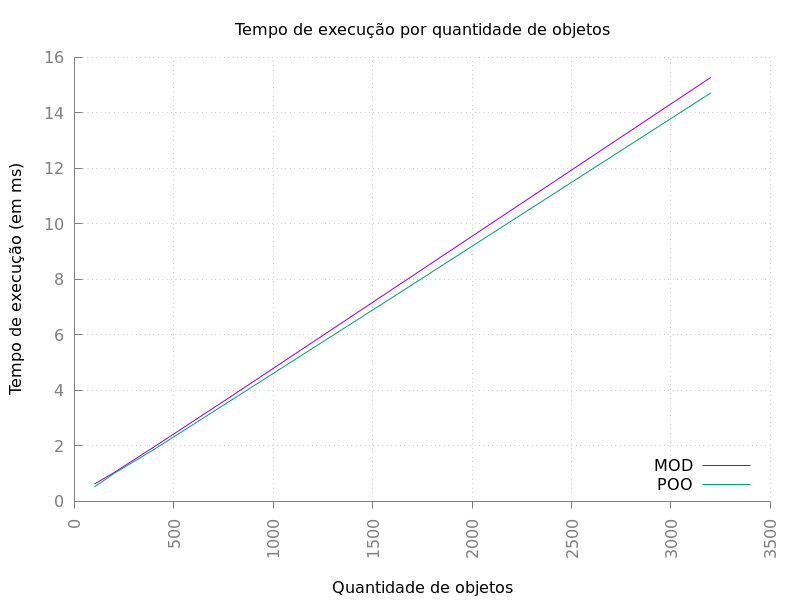
\includegraphics[width=\textwidth]{../figuras/drawv1graph}
        \caption{M�todo \textit{draw}.}
        \label{drawv1graph}
    \end{subfigure}
    \begin{subfigure}[b]{\textwidth}
        \begin{subfigure}[b]{.5\textwidth}
            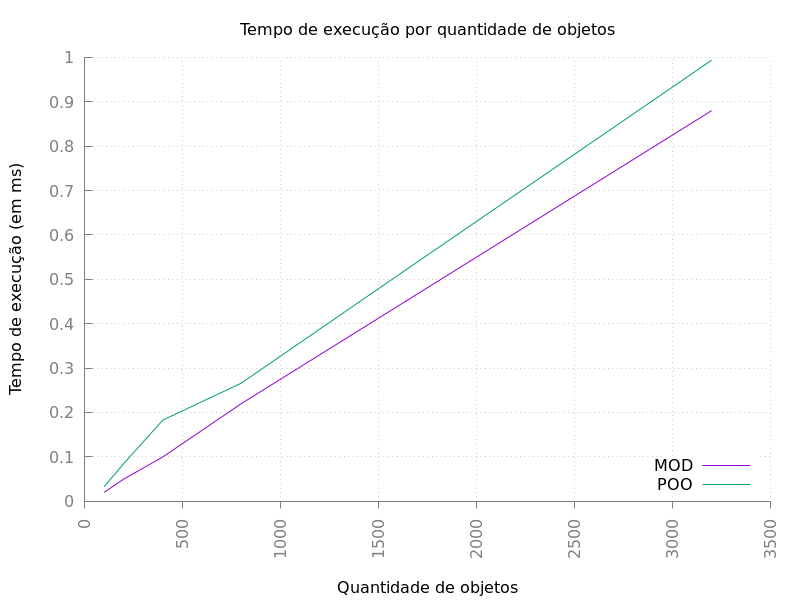
\includegraphics[width=\textwidth]{../figuras/updatev1graph}
            \caption{M�todo \textit{update}}
            \label{updatev1graph}
        \end{subfigure}
        \begin{subfigure}[b]{.5\textwidth}
            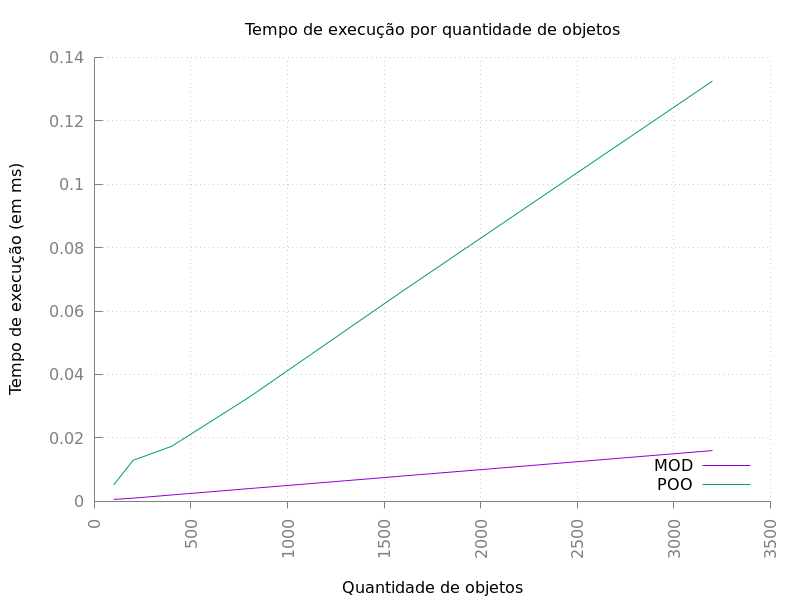
\includegraphics[width=\textwidth]{../figuras/colisionv1graph}
            \caption{M�todo de vef. de colis�o}
            \label{colisionv1graph}
        \end{subfigure}
    \end{subfigure}
    \par\medskip
    \label{v1graphs}
\end{figure}

Os gr�ficos~\ref{drawv1graph},~\ref{updatev1graph} 
e~\ref{colisionv1graph} corroboram o comportamento descrito nessa 
se��o, onde o ganho de desempenho da vers�o OD aumenta conforme 
o n�mero de propriedades requeridas para uma fun��o diminui.

\section{Problema B: renderiza��o de objetos com quatro n�veis de hierarquia}

No problema B os objetos da cena seguem um padr�o de hierarquia, 
diferentemente do problema A, onde todos os n�s do grafo de cena 
s�o filhos do n� raiz. A hierarquia constru�da no problema B segue 
um padr�o no qual uma �rvore � formada a cada quatro objetos onde 
cada objeto est� em um n�vel diferente da �rvore. A quantidade de 
n�veis de hierarquia foi julgada fact�vel pois um objeto com 
quatro n�veis de hierarquia n�o � algo incomum em jogos 3D modernos.

\begin{figure}[h]
    \centering
    \captionof{figure}{Esquema de hierarquia de n�s do problema B.}
    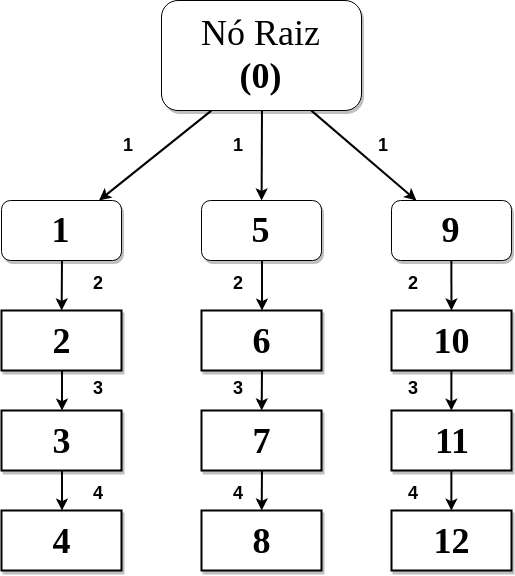
\includegraphics[width =.7\textwidth]{../figuras/problemBscheme}
    \par\medskip
    Fonte: autoria pr�pria
    \label{problemBscheme}
\end{figure}

A figura~\ref{problemBscheme} exemplifica o esquema de hierarquia 
de n�s do problema B para um exemplo de entrada com 12 objetos na 
cena. Esse esquema de hierarquia diminui consideravelmente a 
efici�ncia do m�todo \textit{draw} da vers�o OO do motor, que 
devido a sua natureza recursiva, sofre muitas interrup��es no 
fluxo de execu��o do programa. 

\begin{table}[h!]
\centering
\caption{Tempo m�dio de execu��o das fun��es para a vers�o OO.}
\label{oodv2table}
\begin{tabular}{ccccccc}
                                      & \multicolumn{2}{c}{Draw}                                     & \multicolumn{2}{c}{Att. objetos}                             & \multicolumn{2}{c}{Verif. colis�es}        \\
\multicolumn{1}{l}{N�mero de objetos} & \multicolumn{1}{l}{M�dia} & \multicolumn{1}{l}{Desv. padr�o} & \multicolumn{1}{l}{M�dia} & \multicolumn{1}{l}{Desv. padr�o} & M�dia   & \multicolumn{1}{l}{Desv. padr�o} \\
100                                   & 1.02ms                    & 0.01                             & 0.03ms                    & 0.002                            & 0.004ms & $7 x 10^{-3}$                    \\
200                                   & 1.94ms                    & 0.08                             & 0.08ms                    & 0.003                            & 0.01ms  & 0.004                            \\
400                                   & 3.76ms                    & 0.06                             & 0.21ms                    & 0.01                             & 0.02ms  & 0.006                            \\
800                                   & 7.46ms                    & 0.05                             & 0.42ms                    & 0.03                             & 0.036ms & 0.001                            \\
1600                                  & 14.93ms                   & 0.09                             & 0.8ms                     & 0.02                             & 0.064ms & 0.001                            \\
3200                                  & 29.87ms                   & 0.14                             & 1.5ms                     & 0.02                             & 0.131ms & 0.007
\end{tabular}
\end{table}

\begin{table}[h!]
\centering
\caption{Tempo m�dio de execu��o das fun��es para a vers�o OD.}
\label{dodv2table}
\begin{tabular}{ccccccc}
                                      & \multicolumn{2}{c}{Draw}                                     & \multicolumn{2}{c}{Att. objetos}                             & \multicolumn{2}{c}{Verif. colis�es}                \\
\multicolumn{1}{l}{N�mero de objetos} & \multicolumn{1}{l}{M�dia} & \multicolumn{1}{l}{Desv. padr�o} & \multicolumn{1}{l}{M�dia} & \multicolumn{1}{l}{Desv. padr�o} & M�dia           & \multicolumn{1}{l}{Desv. padr�o} \\
100                                   & 0.54ms                    & 0.02                             & 0.03ms                    & 0.002                            & $6 x 10^{-3}$ms & $2 x 10^{-4}$                    \\
200                                   & 1.04ms                    & 0.01                             & 0.07ms                    & 0.006                            & 0.001ms         & $2 x 10^{-3}$                    \\
400                                   & 1.95ms                    & 0.01                             & 0.18ms                    & 0.01                             & 0.004ms         & 0.003                            \\
800                                   & 3.85ms                    & 0.04                             & 0.38ms                    & 0.02                             & 0.05ms          & 0.03                             \\
1600                                  & 7.62ms                    & 0.03                             & 0.69ms                    & 0.01                             & 0.008ms         & $2 x 10^{-3}$                    \\
3200                                  & 15.29ms                   & 0.06                             & 1.31ms                    & 0.01                             & 0.01ms          & $2 x 10^{-3}$
\end{tabular}
\end{table}

Os resultados contidos nas tabelas~\ref{oodv2table} 
e~\ref{dodv2table} indicam que o c�lculo sequencial de coordenadas 
globais na vers�o OD do motor � uma alternativa mais resiliente � 
mudan�as na hierarquia do grafo de cena, permanecendo com um tempo 
m�dio de execu��o est�vel ap�s a mudan�a. O m�todo \textit{draw}
da vers�o OO por outro lado, teve um acr�scimo consider�vel no 
tempo de execu��o, com uma m�dia de 51\% mais lento do que a 
vers�o OO no problema A e a vers�o OD no problema B. Como a �nica 
diferen�a entre o problema A e o problema B est� na hierarquia de 
n�s, n�o houveram mudan�as significativas no tempo de execu��o 
das fun��es de atualiza��o de objetos e detec��o de colis�es.

\begin{figure}[h!]
    \centering
    \captionof{figure}{Gr�fico comparativo das fun��es \textit{draw} das duas vers�es para o problema B.}
    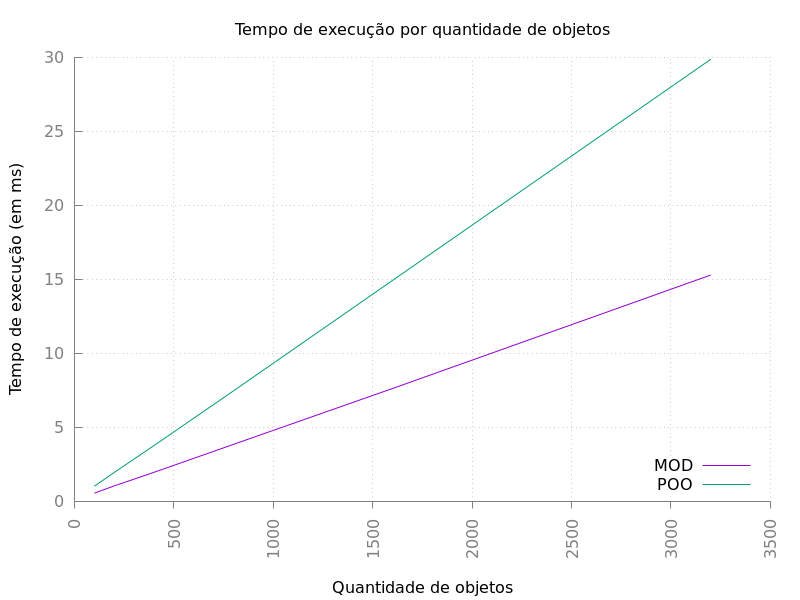
\includegraphics[width =\textwidth]{../figuras/drawv2graph}
    \par\medskip
    Fonte: autoria pr�pria
    \label{drawv2graph}
\end{figure}

A figura~\ref{drawv2graph} cont�m apenas o gr�fico de tempo 
para a fun��o \textit{draw} do problema B, pois foi a �nica em 
que houve mudan�as significativas em rela��o ao problema A. O 
tempo m�dio de execu��o para a vers�o OD permaneceu quase 
inalterado, enquanto que para a vers�o OO, apesar de ter 
mantido o comportamento linear, houve um acr�scimo consider�vel.

\section{Considera��es finais do cap�tulo}

Neste cap�tulo foi testado o desempenho da modelagem orientada 
a dados, a abordagem de programa��o estudada neste trabalho. 
Analisando os resultados obtidos no cap�tulo~\ref{resultscap} e 
os conceitos discutidos na se��o~\ref{secdataorienteddesign}, 
pode ser conclu�do que a MOD n�o garante uma melhora no desempenho, 
por�m fornece um maior controle sobre este. Tendo o conhecimento de 
como os dados est�o armazenados na mem�ria e como estes ser�o 
utilizados permite ao desenvolvedor implementar os procedimentos 
da aplica��o maximizando a efici�ncia da comunica��o entre o 
CPU e a mem�ria.

A convers�o do motor da abordagem orientada a objetos para a vers�o 
orientada a dados apresentou alguns desafios. O primeiro, j� mencionado 
no cap�tulo~\ref{relatedworkscap}, foi a falta de material a respeito 
de MOD. O segundo desafio foi desenvolver a vers�o OD com uma mentalidade 
diferente do modelo de classe e objeto, o qual os desenvolvedores de 
jogos j� est�o mais familiarizados.

Por fim, o maior desafio est� no fato de que a abordagem orientada a dados 
requer uma constante preocupa��o sobre como os dados est�o alocados na 
mem�ria e como estes s�o acessados, o que requer uma escolha para as 
estruturas de dados utilizadas. Isso pode ser facilitado ao se 
determinar o fluxo de dados e quais s�o as transforma��es necess�rias 
nestes, dividindo-as em subfun��es nas quais s� sejam usadas propriedades 
pr�ximas uma da outra na mem�ria. Por�m esse processo de escolha 
das estruturas e das transforma��es n�o � trivial e em muitos casos a 
divis�o n�o � poss�vel, pois muitas propriedades precisam ser utilizadas ao 
mesmo tempo.

Conforme visto na se��o~\ref{secdataorienteddesign}, h� duas maneiras de se 
alocar os dados: o padr�o AoS e o SoA, os quais possuem suas respectivas 
vantagens e desvantagens, cabendo ao desenvolvedor determinar qual padr�o 
� mais adequado para cada conjunto de dados espec�fico. 

\chapter{Considera\c{c}\~oes parciais e Trabalhos Futuros}

\section{Escolha de Uma Arquitetura Adequada Para o Motor}

\section{Escolha Definitiva das Métricas para Medidas de Desempenho}


\bibliographystyle{abnt-alf}
\bibliography{../4_pos_texto/bibliografia}

%\input{../4_pos_texto/anexo}
%\input{../4_pos_texto/apendice}

\end{document}
